% !TeX spellcheck = en_US
\documentclass[IWBstudentthesis%     style
              ,optCharter%           font
              %,optCMYK%             color model
              ,optBiber% 	         bibliography tool
              ,optBibstyleAuthorYear %iwb citation style
              %,optBibstyleNumeric
              ,optEnglish% 		 language
              %,optTikzExternalize%  compiles faster for large tikz images
              ]{IWBlatex}%
%
% Set paths
%\pdfcompresslevel=0
%\pdfobjcompresslevel=0

\usepackage{subfig}
\usepackage{comment}
\usepackage{setspace}
\usepackage{siunitx}
\usepackage{mathtools}
\usepackage{amsmath}

\onehalfspacing
\usepackage{float}
\usepackage{subfig}
\graphicspath{{figures/}}%
\addbibresource{source/literature.bib}%
\makenoidxglossaries%
\newacronym{iwb}{\textit{iwb}}{Institut für Werkzeugmaschinen und Betriebswissenschaften}%
\newacronym{CAM}{CAM}{Computer-aided manufacturing}%done
\newacronym{CAD}{CAM}{Computer-aided design}%done
\newacronym{AM}{AM}{Additive maufacturing}%done
\newacronym{FDM}{FDM}{Fused deposition modeling}%done
\newacronym{WAAM}{WAAM}{Wire arc additive manufacturing}%done
\newacronym{CNC}{CNC}{Computer numerical control}% \acrshort{CNC}
\newacronym{DoF}{DoF}{Degree of freedom}%\acrshort{DoF}
\newacronym{SLA}{SLA}{Stereolithography}%\acrshort{SLA}
\newacronym{SLM}{SLM}{Selective laser melting}%\acrshort{SLM}
\newacronym{DED}{DED}{Directed energy deposition}%\acrshort{DED}
\newacronym{GMAW}{GMAW}{Gas metal arc welding}%\acrshort{GMAW}
\newacronym{CMT}{CMT}{Cold Metal Transfer}%\acrshort{CMT}
\newacronym{CAE}{CAE}{Computer-aided engineering}%\acrshort{CAE}
\newacronym{ERP}{ERP}{Enterprise resource planning}%\acrshort{ERP}
\newacronym{PSO}{PSO}{Particle swarm optimization}%\acrshort{PSO}
\newacronym{TWA}{TWA}{Twist decomposition approach}%\acrshort{TWA}
\newacronym{ML}{ML}{Machine Learning}%\acrshort{ML}
\newacronym{AI}{AI}{Artificial Intelligence}%\acrshort{AI}
\newacronym{RNN}{RNN}{Recurrent neural-network}%\acrshort{RNN}
\newacronym{API}{API}{Application programming interface}%\acrshort{API}
\newacronym{DH}{DH}{Denavit-Hartenberg}%\acrshort{DH}
\newacronym{TCP}{TCP}{Tool center point}%\acrshort{TCP}
\newacronym{MBS}{MBS}{Multi-body simulations}
\newacronym[\glslongpluralkey={Arbeitspakete}]{ap}{AP}{Arbeitspaket}%%
%\newglossaryentry{latex}%
{%
	name=Latex,%
	description={Generische Mark-up-Sprache zum Erstellen wissenschaftlicher Texte. Sie ist in jeder Hinsicht Word überlegen, welches einem visuellen Mark-Up entspricht. Das X von \LaTeX\ wird als ç (Stimmloser palataler Frikativ) ausgesprochen, vergleiche deutsche Aussprache von \textit{ch}.}%
}%
\newglossaryentry{tutorial}%
{%
	name=Tutorial,%
	description={Kurze Gebrauchsanleitung welche ein Thema, einen gewissen Vorgang oder eine Funktion erklärt. Hat nicht den Anspruch auf Vollständigkeit.}%
}%
\newglossaryentry{tikz}%
{%
	name=Ti\textit{k}Z,%
	description={Frontend-Paket, das auf PGF-Plot aufbaut und zum Erstellen von Graphiken dient.}%
}%%

\DeclareCiteCommand{\cite}[\mkbibparens]
{\usebibmacro{prenote}}%
{\usebibmacro{citeindex}%
\printtext[bibhyperref]{\usebibmacro{cite}}}%
{\multicitedelim}
{\usebibmacro{postnote}}

%
\begin{document}%
% Titlepage
% ---------
\frontmatter%
% Info: replace Prof. Daub by Prof. Zäh:\IWBnamesProfZaeh \newline \IWBlangChairMWIWBLWF
% Info: separate multiple supervisors by \newline

% Methodischer Ansatz zur Analyse von Prozessparametern und Optimierung von Randbedingungen in Multi-Achs-Roboterprogrammen

%Methodical Approach for Analyzing Process Parameters and Optimizing Boundary Conditions in Multi-Axis Robot Programs

\IWBstudentthesisTitlePageCustomMastersThesis{Methodischer Ansatz zur Analyse von Prozessvariablen und Optimierung von Randbedingungen in Multi-Achs-Roboterprogrammen}{Methodical Approach for Analyzing Process Variables and Optimizing Boundary Conditions in Multi-Axis Robot Programs}
{Jan Nalivaika \newline Lerchenauerstrasse 10 \newline 80809 Munich}{\IWBnamesProfZaeh \newline \IWBlangChairMWIWB}{\IWButilsDate{01}{03}{2024}}%
%
%\IWBstudentthesisTitlePageCustomBachelorsThesis{German Title}{English Title}{Martin Mustermann \newline Musterweg 20 \newline 80999 München}{\IWBnamesProfDaub \newline \IWBlangChairMWIWBPE}{\IWButilsDate{1}{1}{2018}}%
%
%\IWBstudentthesisTitlePageCustomSemesterThesis{German Title}{English Title}{Martin Mustermann \newline Musterweg 20 \newline 80999 München}{\IWBnamesProfDaub \newline \IWBlangChairMWIWBPE}{\IWButilsDate{1}{1}{2018}}%
%
%\IWBstudentthesisTitlePageCDIDP{German Title}{English Title}{Martin Mustermann \newline Musterweg 20 \newline 80999 München}{\IWBnamesProfDaub \newline \IWBlangChairMWIWBPE}{\IWButilsDate{1}{1}{2018}}%
%\chapter*{Acknowledgment}
Shout-out To the top G's 
%
%
% Task formulation
% ----------------
%% Deckblatt
\chapter*{Scope of Work}

%\markright{Aufgabenstellung} 	% Kolumnentitel manuell auf "Aufgabenstellung"

\textbf{Title of the Master's Thesis:}\\
\Large{Methodical Approach for Analyzing Process Parameters and Optimizing Boundary Conditions in Multi-Axis Robot Programs}\\
\newline
\normalsize{\textbf{Titel der Master's Thesis:}}\\
\Large{Methodischer Ansatz zur Analyse von Prozessparametern und Optimierung von Randbedingungen in Multi-Achs-Roboterprogrammen}
\normalsize

\begin{tabbing}
	\hspace{7em} 		\= \hspace{13em}			\= \hspace{7em} 		\= \kill
				\> 						\> \\
	\textbf{Author:} \>  Jan Nalivaika	\> \textbf{Supervisor:} 	\>Ludwig Siebert  \\
	\textbf{Issue:} 	\> 02.10.2023	\> \textbf{Submission:} 	\> 29.03.2024
\end{tabbing}

\vspace{5mm}
\textbf{Motivation:}\\
Computer-aided manufacturing (\acrshort{CAM}) is used to automatically generate tool paths for 
computer numerically controlled machines. The \acrshort{CAM} software considers the models of the 
raw and finished parts, the constraints of the machine, the tools, and the manufacturing 
technology. Together with user-configurable parameters, tool paths for 3-axis, 5-axis, and 
robot-based machine tools are generated. The growing demand for flexibility in machine tools, 
such as the use of multiple manufacturing technologies in one machine or automated loading 
and unloading, has led to many machine tools being equipped with additional mechanical 
axes. Examples include robots mounted on linear axes and rotary-tilt tables.
The tool paths created in \acrshort{CAM} programs are usually defined by five degrees of freedom. The 
first three are the translational axes X, Y, and Z. The tilting and inclining of the tool are defined 
by the A- and B-axes. Occasionally, an additional rotation of the tool (C-axis) around the Z-axis (e.g., for dragging a swivel knife) is defined. Machines with more degrees of freedom than 
those limited by the toolpath often need user-defined constraints. These constraints are 
necessary to fully specify the movements of the machine axes. An example is the alignment 
of a part using the rotary-tilt table so that the Z-axis of the tool always points in the direction of 
gravity. This is helpful in processes like fused deposition modeling (\acrshort{FDM}) and wire arc additive 
manufacturing (\acrshort{WAAM}).
It is common practice to set the user-defined constraints based on experience. The definition 
of these constraints does not affect the relative tool path generated by the \acrshort{CAM} software. A 
preliminary literature review indicates that the configuration of these degrees of freedom has 
an impact on the energy demand and stability of the process. As such, a methodical approach to optimize these constraints in terms of 
efficiency, speed, and energy demand of the machine is required. Currently, no literature
provides a comprehensive analysis or methodology regarding this global optimization 
problem.

\vspace{5mm}
\textbf{Objective:}\\
This work aims to attain a methodical approach that analyzes a set of constraints and 
evaluates the influence of those constraints on a set of defined process variables. It will focus
on a 6-axis robot with a rotary-tilt table, whereby the results should also be transferable to other machines. Furthermore, the experiments and validations will be limited to the 
manufacturing processes of \acrshort{WAAM} and milling.
First, the influence of the constraints on relevant process variables (energy demand, joint 
turnover, speed and acceleration peaks, and total joint movements) in a manufacturing 
process such as \acrshort{WAAM} will be assessed. Subsequently, a process evaluation will be
elaborated in the \acrshort{CAM} software, by means of which the process quality can be determined.
Depending on the respective process variables, approximation or machine learning methods 
will be investigated for the process evaluation. The process quality as a one-dimensional 
variable will be determined by weighting the process variables. Subsequently, a method for 
the optimization of the constraints will be elaborated. This task corresponds to an optimization 
problem in which the process quality will be maximized by selecting suitable constraints.\newline


\vspace{5mm}
\textbf{Procedure and working method:}\newline

The following work packages are conducted within this thesis:

\begin{itemize}
\item Literature research
\item Familiarization with \acrshort{WAAM}, milling machines, and \acrshort{CAM} software
\item Selection of suitable process parameters
\item Elaboration of the proposed method in a suitable programming language
\item Verification and validation of the elaborated method
\item Documentation of the work

\newpage	 
\end{itemize}
\vspace{1.0cm}
\textbf{Agreement:}\\

Through the supervision of B.Sc. Jan Nalivaika intellectual property of the \textit{iwb} is incorporated in this work. Publication of the work or transfer to third parties requires the permission of the chair holder. I agree to the archiving of the work in the library of the \textit{iwb}, which is only accessible to \textit{iwb} staff, as inventory and in the digital student research project database of the \textit{iwb} as a PDF document.
\vfill

\IWBaddressCityChair, \textcolor{red}{29.03.2024 WHAT DATE GOES HERE ?????????????????????????????????????????????}
\vspace{2.5cm}\\
\begin{tabular}{p{0.5\linewidth}p{0.5\linewidth} }
	Prof. Dr.-Ing.		& B.Sc.\\
Michael F. Zäh  	& Jan Nalivaika
\end{tabular}
%% ADD ME !!!!!!!!!!!!!!!!!!!!
%
% Abstract
% --------
%% !TeX spellcheck = en_US
% In total max. 1 Page!
\IWBstudentthesisAbstract{%
%
% Abstract English:
This thesis discusses a methodology for analyzing and optimizing process variables in manufacturing systems with redundant \acrshort{DoF}s. The main focus lies on a 6-\acrshort{DoF} industrial robot that traverses a toolpath defined in 5-\acrshort{DoF}s (X,Y,Z,A,B). This means that the rotation C, which represents the rotation around the tool symmetry axis, is a redundant \acrshort{DoF} and can be chosen freely. The first part of the methodology covers the analysis of process variables, such as direction changes in the joints or the total travel of the joints. The goal is to understand how the redundant \acrshort{DoF}s affect the robot's behavior and how they can be used to optimize user-selected process variables. The second part of the methodology proposes a procedure to optimize the user-selected process variables by properly constraining the redundant \acrshort{DoF}. After modeling the robot in Python, validation is performed on multiple toolpaths. The results show that the redundant \acrshort{DoF}s can significantly affect the process variables. By implementing a \acrshort{PSO} algorithm, it is possible to find the ideal setting for the redundant \acrshort{DoF}s, thus maximizing the process quality with respect to the process variables. 
}
{%
	%
	% Zusammenfassung Deutsch:
	In dieser Arbeit wird eine Methodik zur Analyse und Optimierung von Prozessvariablen in Fertigungssystemen mit redundanten Freiheitsgraden diskutiert. Der Schwerpunkt liegt auf einem Industrieroboter mit sechs Freiheitsgraden, der eine in Werkzeugpfad abfährt, der nur fünf Freiheitsgrade (X, Y, Z, A, B) definiert. Dies bedeutet, dass die Rotation um Achse C, die die Werkzeugsymmetrieachse darstellt, ein redundanter Freiheitsgrad ist und frei gewählt werden kann. Der erste Teil der Methodik umfasst die Analyse von Prozessvariablen wie Richtungswechsel in den Gelenken oder der Gesamtverfahrwege der Gelenke. Das Ziel ist es, zu verstehen, wie sich die redundanten Freiheitsgrade auf das Verhalten des Roboters auswirken und wie sie zur Optimierung der vom Benutzer ausgewählten Prozessvariablen verwendet werden können. Der zweite Teil der Methodik schlägt ein Verfahren zur Optimierung der ausgewählten Prozessvariablen vor. Nach der Modellierung des Roboters in Python wird die Validierung anhand mehrerer Werkzeugbahnen durchgeführt. Die Ergebnisse zeigen, dass die redundanten Freiheitsgrade die Prozessvariablen erheblich beeinflussen können. Durch die Implementierung eines \acrshort{PSO}-Algorithmus ist es möglich, die ideale Einstellung für die redundanten Freiheitsgrade zu finden und somit die Prozessqualität in Bezug auf die Prozessvariablen zu maximieren.
	
	
}%
%
%
%% ADD ME !!!!!!!!!!!!!!!!!!!!
%
% Content
% -------
\IWBstudentthesisPrintTableOfContents%
%
% List of Abbreviations
% ---------------------
\printnoidxglossary[type=acronym,sort=standard,title={\IWBlangAcronyms}]
%
% Mainmatter
% ----------
\mainmatter%
%% !TeX spellcheck = de_DE
\chapter{LaTeX-Tutorial}%
Dieses \gls{tutorial} liefert eine Kurzeinführung in die Verwendung von \gls{latex}.%
%
\section{Titelseite}%
Die Titelseite wird in {./main.tex} definiert. Der Studienarbeitstyp wird durch Ein- und Auskommentieren der Befehle%
\begin{itemize}%
	\item \verb|\IWBstudentthesisTitlePageCustomMastersThesis|,%
	\item \verb|\IWBstudentthesisTitlePageCustomBachelorsThesis| und%
	\item \verb|\IWBstudentthesisTitlePageCustomSemesterThesis|%
\end{itemize}%
ausgewählt und die Seite entsprechend der Argumente gesetzt. Die Professoren und Lehrstuhle können mittels der Makros%
\begin{itemize}%
	\item \verb|\IWBnamesProfReinhart \newline \IWBlangChairMWIWBLBM| oder%
	\item \verb|\IWBnamesProfZaeh \newline \IWBlangChairMWIWBLWF|%
\end{itemize}%
ausgewählt werden.%
%
\section{Zitation}%
%
Zum Zitieren stehen die Standartbefehle \verb|\textcite| und \verb|\parencite| zur Verfügung. Soll der Autorename im Satz verwendet werden, eignet sich ersteres, z.B. \textcite[2-3]{Bayerlein2018} bezieht sich auf \textcite{Bayerlein2016469}. Soll das Zitat in Klammern nach die Aussage gestellt werden empfiehlt sich zweiteres \parencite{Zaeh2018385}. Sammelzitationen am Satzende schreiben sich wie folgt \parencite{Kleinwort2018658,Kleinwort20189,Kleinwort2018631}. Die Zitation von Online-Quellen kann schwierig sein, da nicht immer der Autor und das Erscheinungsjahr verfügbar sind. Vergleicht man \textcite{Heuss2018} und \textcite{iwb-Startseite}, stellt man fest, dass bei zweiteren der Seitentitel statt des bekannten Schemas eingesetzt wird.\par%
%
Normen werden als \textcite{ISO.10218-2} dargestellt. Im Bibtex-Export des verwendeten Literaturverwaltungsprogramm sind bestimmte Einstellungen vorzunehmen. Dokumententyp ist \enquote{@book} mit folgenden Einträgen:
\begin{itemize}
	\item Normtyp und Nummer als \enquote{title}
	\item Langtitel als \enquote{subtitle}
	\item Verlag als \enquote{publisher}
	\item Jahr als \enquote{date}
	\item \enquote{author} darf nicht belegt werden!
\end{itemize}
%
\section{Abkürzungen}
In {./source/abbreviations.tex} können Abkürzungen definiert werden. Es gibt Besonderheiten zu Ausdrücken, deren Pluralendung nicht auf s endet. Hier müssen ggf. Kurz- und Langformen des Ausdrucks auch für den Plural definiert werden.\par%
\begin{itemize}
	\item \verb|\gls{ros}|: schreibt beim ersten Auftreten im Dokument ausführlich \gls{ros}, ab dem zweiten Auftreten wird abgekürzt \gls{ros}% 
	\item \verb|\glspl{ap}| verwendet den Plural in Langform \glspl{ap} und danach in Kurzform \glspl{ap}%
\end{itemize}%
%
\section{Glossar}
In {./source/glossary.tex} können Begriffe erklärt, abgegrenzt oder definiert werden. Begriffe erhalten einen Namen und eine Beschreibung als Glossareintrag sowie ein Lable zum Referenzieren im Text. Ein Glossar ist Optional.\par%
\begin{itemize}%
	\item \verb|\gls{latex}|: Schreibt den Namen aus dem Glossarverzeichnis mit Verweis auf den Glossareintrag \gls{latex}%
\end{itemize}%
%
\section{Abbildungen}
Graphiken und Bilder können in beliebigen Dateiformaten eingebunden werden, vergleiche \cref{fig:MyImage}. Vektorgraphiken sind im Allgemeinen Pixelgraphiken in Schärfe und Speicherbedarf überlegen.\par%
%
\begin{figure}[htb]%
    \centering%
    %
    % Including .png
    
\includegraphics[width=40mm]{figures/ImagePNG.png}%
    %
    \hspace*{5mm}%
    %
    % Including .pdf
    
\includegraphics[width=40mm]{figures/ImagePDF.pdf}\par%
    %
    % Including .tikz
    \begingroup%
        %\AMtikzExternalizeSkipNext%
        \resizebox{40mm}{!}{\begin{tikzpicture}[inner sep=0pt, outer sep=0pt]%
    \fill [draw=TUMBlue,line width=5mm,fill=none] (0mm,0mm) rectangle (95mm,95mm);%
    \node at (50mm,50mm) {\fontsize{60}{60}\selectfont TIKZ};%
\end{tikzpicture}%
}%
    \endgroup%
    %
    \hspace*{5mm}%
    %
    % Including .pdf_tex
    \begingroup%
        \def\svgwidth{40mm}%
        \fontsize{25}{25}\selectfont%
        \input{figures/ImagePDFTEX.pdf_tex}%
    \endgroup%
    %
    \caption{Beschreibung des Bilds.\label{fig:MyImage}}%
\end{figure}%
%
\begin{figure}[htb]%
    \centering%
    \small%
\pgfplotstableread{figures/datatable2d.dat}{\datatableTwoDim}%
\begin{tikzpicture}[scale=1]%
    \begin{axis}[width = 9cm, height = 6cm, scale only axis=true%
                 ,xmin = 0%
                 ,xmax = 10%
                 ,xlabel = {$t$ in s}%
                 ,xtick distance = 1%
                 ,ymin = -1.2%
                 ,ymax = 1.2%
                 ,ylabel = {y-Label}%
                 ,ytick distance = 0.5%
                 ,grid = both%
                 ,grid style = {line width = .1pt, draw = TUMBlack!10}%
                 ,legend style = {at = {(0.1cm,0.1cm)}, anchor = south west,font=\small}%
                 ,\IWBlangGerEng{/pgf/number format/use comma}{}%
                 ]%
        \addplot [TUMBlue,very thick] table [x={X}, y={Y1}] {\datatableTwoDim};%
        \addplot [TUMBlue3,very thick,dashed] table [x={X}, y={Y2}] {\datatableTwoDim};%
        \addplot [TUMBlack,very thick,dotted] table [x={X}, y={Y3}] {\datatableTwoDim};%
        \legend{$\sin(t)$,$\cos(t)$,$0.5$};%
    \end{axis}%
\end{tikzpicture}%
%
%
%
    \caption{Beschreibung des Plots.\label{fig:PlotTwoDim}}%
\end{figure}%
%
Für Nutzer mit perfektionistischen Anspruch empfiehlt sich die Nutzung von \gls{tikz}. Vorteil ist, dass die Erzeugung von Daten und die Darstellung komplett getrennt werden. Die Darstellung erfolgt einheitlich gemäß eines generischen Mark-Ups, vergleiche \cref{fig:PlotTwoDim,fig:PlotThreeDim}.\par%
%
\begin{figure}[htb]%
    \centering%
    \small%
\pgfplotsset{colormap={mycolormap}{rgb255=(255,255,0) rgb255=(255,0,0)}}%    
\begin{tikzpicture}%
    \begin{axis}[width = 10cm, height = 8cm%
                ,xmin = -1%
                ,xmax = 1%
                ,xlabel = {$x$ in m}%
                ,xtick distance = 0.5%
                ,ymin = -1%
                ,ymax = 1%
                ,ylabel = {$y$ in m}%
                ,ytick distance = 0.5%
                ,zmin = 0%
                ,zmax = 1%
                ,zlabel = {$z$ in m}%
                ,ztick distance = 0.2%
                ,grid = both%
                ,grid style = {line width = .1pt, draw = TUMBlack!10}%
                ,colorbar%
                ,view={60}{30}%
                ,\IWBlangGerEng{/pgf/number format/use comma}{}%
                ]%
        \addplot3 [surf,z buffer=sort] table[x={X}, y={Y}, z={Z}] {figures/datatable3d.dat};%
    \end{axis}%
\end{tikzpicture}%
%
%
%
    \caption{Beschreibung des Plots.\label{fig:PlotThreeDim}}%
\end{figure}%
%
%
%
%% !TeX spellcheck = en_US
\chapter{Introduction}%
\section{Motivation}%

In the age of "Industrie 4.0", advanced technologies like digital twins, have greatly transformed industrial manufacturing~\cite{Singh.2021}. A considerable amount of data can be gathered from various processes, like milling or 3D printing. By analyzing this data, it is possible to find new and optimized methods for improving efficiency as well as streamline and enhancing the manufacturing process~\cite{Ghobakhloo.2020}. By doing so, a significant amount of resources, like time and money, can be saved while at the same time increasing the quality of the produced product~\cite{Bibby.2018,Simonis.2016}.
Computer-aided manufacturing (\acrshort{CAM}) has been introduced as a crucial tool to improve productivity and accuracy in creating customized products~\cite{Feldhausen.2022}. \acrshort{CAM} systems automate and optimize tasks such as machining, welding, and assembly~\cite{LalitNarayan.2013b}. One of the key strengths of \acrshort{CAM} lies in its precision and consistency, ensuring that intricate components are produced with minimal error. Furthermore, \acrshort{CAM} systems contribute to increased efficiency by minimizing material waste and reducing production time~\cite{Dubovska.2014}. These capabilities play a significant role in achieving a carbon-neutral production process~\cite{Saxena.2020}. One of the most important areas of \acrshort{CAM} is the calculation of the tool path for computer numerical control (\acrshort{CNC}) machines as well as the movement and behavior of multi-axis industrial robots~\cite{Pan}. 


Manufacturing machines are the backbone of modern industrial processes~\cite{Bi.2020}. These machines encompass a wide range of equipment, from \acrshort{CNC} machining centers to 3D printers and automated assembly lines. Their primary ability lies in precision ($\mu$m-scale) and efficiency \cite{Liberman.2021}. \acrshort{CNC} machines, for instance, can repeatedly produce intricate parts with high accuracy, reducing human error and ensuring consistency~\cite{Jia.2018}. 

Industrial robots are a dominant part in the area of manufacturing as they can perform multi-axis movements. These capabilities are especially helpful to fulfill the customers wishes for individualized products~\cite{Sherwani.2020}. They are cheaper to acquire and more flexible compared to \acrshort{CNC} milling machines, but have their own set of disadvantages like for example lower stiffness~\cite{Iglesias.2015, Liberman.2021}. One of the most important advantages of industrial robots is their wide adaptability. They allow for quick reconfiguration to produce different components or products, promoting flexibility in manufacturing~\cite{Billard.2019}. Further, advancements in robotics and Artificial Intelligence (\acrshort{AI}) have broadened their capabilities, enabling tasks that were once deemed too complex or hazardous for humans~\cite{Goel.2020}. 
For achieving better efficiency and continuous sustainability in the current fast-changing environment requires a thorough analysis of the interdependent relationships between the manufactured part, process parameters, and boundary conditions that govern multi-axis robot programs~\cite{Pan, Gadaleta.2019}. As the companies that work with industrial robots can place a strong emphasis on energy reduction, cycle-time minimization, or precision, optimizing these parameters is essential. \acrshort{CAM} enables the simulation of the planned process, thus adapting any boundary conditions to fit the selected goals~\cite{Kyratsis.2020,Maiti.2017,Pan,Uhlmann.2016}.
This thesis is focused on a methodical approach for analyzing process parameters and optimizing boundary conditions in multi-axis robot programs. 

\section{Problem Formulation}\label{Problem Formulation}
Manufacturing systems that incorporate redundant degrees of freedom (\acrshort{DoF}s) offer significant advantages in terms of flexibility and adaptability~\cite{Anjum.2022}. One example of a system with redundancy is a 6-\acrshort{DoF} industrial robot with a rotary tilt table, which brings the system to eight \acrshort{DoF}. However, these systems also present various conflict points that need to be carefully managed to ensure optimal performance~\cite{Boscariol.2020, Wang.2022}.


One of the critical challenges in manufacturing systems with redundant \acrshort{DoF}s is singularity avoidance~\cite{ Kireanski.1993, Wang.2022}. Singularities, which are critical points in the motion of a robot manipulator, arise when the system loses its ability to maintain full control or achieves limited mobility as a consequence of specific joint configurations~\cite{Malyshev.2022}. These configurations result in the loss of a \acrshort{DoF} or make the system highly sensitive to small changes, leading to unstable or even unpredictable and dangerous behavior~\cite{Zhao.2021, Milenkovic.2021}. Limiting the possible positions by adding artificial constraints can help to avoid this problem~\cite{Faria.2018}. %Advanced control algorithms and motion planning techniques are necessary to detect and avoid singularities, ensuring the system operates within safe and stable regions.

%Redundant degrees of freedom introduce complexities in controlling joint accelerations and jerks. Rapid changes in acceleration and jerk can cause mechanical stress, decrease system lifespan, and compromise precision. Proper trajectory planning and control schemes that consider joint acceleration and jerk limits are crucial to maintain smooth and controlled motion, reducing the risk of mechanical failures and ensuring accurate positioning.

%Extension:
%Redundant degrees of freedom can provide additional extension capabilities to industrial robots, allowing them to reach difficult-to-access areas. However, managing and controlling the extension can be challenging, particularly when precise positioning or maintaining stability is required. Accurate modeling, control algorithms, and calibration techniques are necessary to ensure proper extension control and to avoid issues related to overextension or underextension.

%Energy Use:
%Redundant degrees of freedom can increase energy consumption in manufacturing systems. Additional joints and actuators require more power, leading to higher energy costs and environmental impact. Efficient energy management strategies, such as optimizing control algorithms, utilizing regenerative braking, and incorporating energy-efficient components, are crucial to minimize energy use while maintaining system performance.

%Direction Changes:
%Redundant degrees of freedom offer increased flexibility in changing the direction of motion. However, abrupt and frequent direction changes can lead to mechanical stress, decreased precision, and increased energy consumption. Proper trajectory planning, smooth path generation, and optimized control algorithms are essential to manage direction changes effectively, ensuring smooth and controlled motion without compromising system performance.

%Transfer Time:
%Transfer time is another critical aspect affected by redundant degrees of freedom. Complex motion patterns required for utilizing redundant degrees of freedom can increase the time required to complete a task. Minimizing transfer time is crucial for improving production efficiency and throughput. Optimal path planning, motion optimization, and parallel processing techniques can be employed to reduce transfer time while leveraging redundant degrees of freedom effectively.

%Precision:
%Redundant degrees of freedom can enhance precision and accuracy in manufacturing systems. However, achieving and maintaining high precision can be challenging due to increased complexity and sensitivity to various factors. Calibration techniques, accurate modeling, feedback control, and error compensation algorithms are vital to ensure precise positioning and improve overall system accuracy.

%Maximum Load Capacity:
%Redundant degrees of freedom can influence the maximum load capacity of industrial robots. Increased complexity and additional joints can affect the robot's ability to handle heavy loads or maintain stability. Proper design considerations, such as structural reinforcement, joint torque and force limitations, and payload distribution, are necessary to ensure safe and reliable operation under maximum load conditions.

%Stiffness:
%The presence of redundant degrees of freedom can affect the stiffness of the manufacturing system. Increased flexibility due to redundant degrees of freedom may introduce compliance and reduce overall system stiffness. This can impact precision, accuracy, and stability. Careful design, utilization of appropriate materials, and control strategies that compensate for compliance can be employed to ensure the desired level of stiffness and system rigidity.


%---------------





One significant aspect of manufacturing systems with redundant \acrshort{DoF}s is joint acceleration and jerk, which is the rate of change of acceleration. The robot must allocate accelerations effectively among its joints to achieve smooth and coordinated motion. Failure to do so can result in jerky or erratic movements, which not only compromise precision but also impact the efficiency of the manufacturing process~\cite{Duong.2021}. Rapid changes in acceleration and jerk can cause mechanical stress, decrease system lifespan, and compromise precision. Additionally, the joints can be limited in their ability to keep up with the required speed due to limitations in power~\cite{Staff.1988}. Therefore, advanced control algorithms and motion planning techniques are necessary to optimize joint motion and minimize conflicts in joint acceleration and jerk~\cite{Duong.2021, Valente.2017}.

Extension control is another critical aspect that needs to be addressed in systems with redundant \acrshort{DoF}s. Redundant \acrshort{DoF}s can provide additional extension capabilities to industrial robots, allowing them to reach difficult-to-access areas~\cite{Duong.2021}. However, managing and controlling the extension can be challenging, particularly when precise positioning or maintaining stability is required~\cite{Lin.2022}.
The robot must accurately determine the appropriate position for each joint to avoid unnecessary over-extension and collisions with the surrounding environment. The robot pose, which is the combination of position and orientation in three-dimensional space, also has a significant effect on robot stiffness~\cite{Xiong.2019}. An increased number of joints can introduce more play and reduce overall system stiffness. This can affect precision, accuracy and stability. Robot pose and its \acrshort{DoF}s must be carefully considered to ensure the desired level of system rigidity~\cite{Wang.2022, Shi.2021}.


Precision is a crucial element in manufacturing systems, and closely tied to its stiffness. The robot needs to have precise control over the movement of each joint to achieve the desired accuracy of positioning in the manufacturing process. Nevertheless, achieving and maintaining high accuracy and repeatability can be difficult due to the increased complexity and sensitivity to various factors~\cite{Duong.2021}. %Any deviations or errors in joint motion can lead to compromised precision and reduced product quality. %To address this, advanced sensing and feedback control mechanisms, such as force/torque sensors and visual feedback systems, can be employed to enhance precision and ensure the accurate execution of manufacturing tasks.
Frequent changes in direction in the joints are another factor that affects precision. 
Due to the serial kinematics of industrial robots, the present play in the motor joints can add up the inaccuracies and impede the manufacturing process~\cite{Huynh.2020, ChenGang.2014}. Mechanical stress, decreased precision, and increased energy consumption can result from abrupt and frequent direction changes~\cite{Gasparetto.2010}.
 
Furthermore, effectively coordinating the movement of multiple joints to execute rapid direction changes can prove to be a difficult and computationally intensive task~\cite{VandeWeghe.2007}. Poor direction changes can result in prolonged and unnecessary movement times, ultimately hampering the overall productivity of the manufacturing process~\cite{Reiter.2016}. %Therefore, advanced control algorithms and motion planning techniques are required to optimize direction changes and minimize transfer time, ensuring efficient and timely execution of manufacturing tasks.
Minimizing production time is crucial for improving efficiency and throughput. Optimal path planning, motion optimization, and parallel processing techniques can be employed to reduce non-value adding movements while leveraging redundant \acrshort{DoF}s effectively, for significant process improvement~\cite{Boscariol.2020}.




Energy use is also a significant concern in manufacturing systems employing redundant \acrshort{DoF}s~\cite{Doan.2016}. The presence of additional joints and their non-optimal usage can require more power to operate, potentially leading to increased energy consumption. As energy efficiency becomes a priority in modern manufacturing, efficient mitigation strategies are necessary~\cite{Boscariol.2020, Boscariol.2019}. 
%energy management strategies are necessary to mitigate the increased power demand

%Maximum load capacity is another area influenced by redundant degrees of freedom. The presence of additional joints can introduce structural limitations, affecting the robot's ability to handle heavy loads. Structural analysis and design considerations are crucial to ensure that the robot's mechanical structure can withstand the required load capacity without compromising its integrity or performance. This may involve using high-strength materials, optimizing structural configurations, and employing robust safety mechanisms to prevent overloading.
\newpage
While redundant \acrshort{DoF}s may introduce potential conflicts and require special attention, they can also significantly enhance performance in manufacturing systems~\cite{Ayten.2016}. The added \acrshort{DoF}s increase flexibility and adaptability, enabling the robot to carry out complex tasks more efficiently. Redundancy enables multiple approaches to achieve a desired end-effector position or orientation. By effectively utilizing the surplus of \acrshort{DoF}s, manufacturing systems can enhance their performance, increase efficiency, and exhibit greater flexibility in handling diverse tasks~\cite{Boscariol.2020}. 

Currently, there is no integrated system that can evaluate a computed tool path based on the chosen objective, such as minimizing movement or maximizing stiffness. %, in conjunction with available \acrshort{CAM} systems.
Additionally, there is no option to provide an optimal or near-optimal solution for defining the necessary constraints for a specific goal like for example, minimizing energy usage while at the same time reducing joint accelerations.


\section{Objective}\label{OBJECTIVE}
The definition of the redundant constraints, mentioned in Chapter \ref{Problem Formulation}, does not affect the relative tool path as generated by the \acrshort{CAM} software. As such, a methodical approach to optimize these constraints without altering the toolpath in terms of efficiency, speed, and energy demand of the machine is required. Currently, no literature provides a comprehensive analysis or methodology regarding this global optimization problem.
This work aims to attain a methodical approach that analyzes a set of constraints and evaluates the influence of those constraints on a set of defined process variables. This work is focused on a 6-axis robot with a rotary-tilt table, whereby the results should also be transferable to other machines. Furthermore, the experiments and validations will be limited to the manufacturing processes of wire arc additive manufacturing (\acrshort{WAAM}) and milling. 


First, the influence of the constraints on relevant process variables (energy demand, joint turnover, speed and acceleration peaks, total joint movements) in a manufacturing process such as \acrshort{WAAM} will be assessed. Subsequently, a process evaluation will be elaborated, by means of which the process quality can be determined. Depending on the respective process variables, approximation methods or machine learning methods will be investigated for the process evaluation. The process quality as a one-dimensional variable will be determined by weighting the process variables. Subsequently, a method for the optimization of the constraints will be elaborated. This task corresponds to an optimization problem in which the process quality will be maximized by selecting suitable constraints. 
%% ADD ME !!!!!!!!!!!!!!!!!!!!
%% !TeX spellcheck = en_US
\chapter{State of Science and Technology}%
The following chapter gives a overview of manufacturing technologies, CAM, and various algorithms for optimization problems. Special attention is given to the comparison of optimization problems in manufacturing with redundant degrees of freedom. 
\section{Manufacturing Technologies}
Manufacturing technologies encompass a wide range of processes that are used to transform raw materials into finished products. Two major categories within this field are subtractive and additive manufacturing \cite{Iqbal.2020}. Subtractive manufacturing involves removing material from a workpiece to shape it into the desired form  \cite{Watson.2015}. This is commonly achieved through techniques like cutting, drilling, milling, or grinding. On the other hand, additive manufacturing, also known as 3D printing, involves building up layers of material to create an object. This process offers greater design flexibility and the ability to create complex geometries  \cite{Dilberoglu.2017}. Both subtractive and additive manufacturing play crucial roles in various industries, revolutionizing production methods and offering new possibilities for customization and innovation  \cite{Bandyopadhyay.2020, vanLe.2017}.











\subsection{Subtractive Manufacturing}
Subtractive manufacturing, also referred to as subtractive fabrication or machining, is a precise and efficient method utilized in contemporary manufacturing processes \cite{Wang.2023}. This approach entails the removal of material from a solid block or workpiece, resulting in the formation of a desired shape or product \cite{Calleja.2018}. In contrast to additive manufacturing techniques, like 3D printing, where material is applied layer by layer, subtractive manufacturing always starts from a block of material \cite{Abdulhameed.2019}.

Subtractive manufacturing involves various techniques such as milling, turning, drilling, and grinding that are performed using computer numerical control (CNC) machines \cite{Kumar.2020}. Such machines are programmed to control cutting tool movement precisely to clear material from the workpiece based on a predetermined design \cite{Amanullah.2017}.

The versatility and precision of subtractive manufacturing is one of its significant advantages. A CNC machine can process a diverse array of materials, such as metals, plastics, and composites, with exceptional precision and surface quality, allowing for the creation of intricate and complex components \cite{Tomaz.2021}. As a result, it finds applications in industries where precision and quality are critical, such as aerospace, automotive, and medical.

The process of subtractive manufacturing starts with the drafting of the intended component using computer-aided design (CAD) software. Subsequently, CAM software is used to generate instructions that are used to guide the CNC machine (see chapter \ref{CAMmain} for more details) . The machining process begins with the machine operator setting up and securing the workpiece in the machine and starting the execution of the generated instructions.

The cutting tools then perform various operations, including drilling holes, creating pockets or slots, and shaping the external contours of the part, by making precise and controlled movements. In a typical 3-axis machine, the degrees of freedom are along the X, Y, and Z axes. Additionally, some machines have advanced abilities like constantly monitor and adjusts the cutting parameters to ensure the most efficient cutting speed, feed rate, and tool engagement while minimizing errors.


Subtractive manufacturing provides numerous advantages over alternative manufacturing techniques. This method allows for the creation of intricate and highly customizable components with tight tolerances and complex geometries \cite{Jayawardane.2023}. In addition, it results in exceptional surface finish, dimensional accuracy, and consistency, guaranteeing uniform quality across production runs. Moreover, it is cost-effective for small to medium production volumes as it does not necessitate the use of costly molds or tooling.

One of the disadvantages of the process can be time-consuming, particularly for intricate designs, and can result in significant material waste. Furthermore, it may not be appropriate for high hardness or brittle materials, which can lead to excessive tool wear or breakage. In summary, subtractive manufacturing offers a wide range of applications but should be carefully considered for each situation. With the ability to produce intricate shapes with superior precision and surface quality, this technology has become indispensable across a variety of industries. Nonetheless, it is crucial to evaluate its restrictions and suitability for specific design needs and material characteristics.


---- 
One of the most important technologies in subtractive manufacturing are CNC machines.
CNC machining, short for Computer Numerical Control machining, is a manufacturing process that utilizes computerized controls and precise machine tools to remove material from a workpiece. This automated process offers numerous advantages over traditional manual machining, including increased accuracy, repeatability, and efficiency.

However, one common issue in CNC machining is tool vibration. Tool vibration refers to the unwanted oscillation or movement of the cutting tool during the machining operation. This phenomenon can have detrimental effects on the quality of the finished part and can lead to various problems, such as poor surface finish, reduced dimensional accuracy, increased tool wear, and even tool breakage.

Several factors contribute to tool vibration in CNC machining. One of the primary factors is the cutting parameters, which include the cutting speed, feed rate, and depth of cut. When these parameters are not optimized, excessive cutting forces can be generated, causing the tool to vibrate. It is crucial to find the right balance between material removal rates and minimizing tool vibration to ensure optimal machining outcomes.

Tool geometry also plays a significant role in tool vibration. The design of the cutting tool, including the shape, rake angle, and clearance angle, affects how the tool interacts with the workpiece material. Improper tool geometry can lead to increased cutting forces and vibrations. Selecting the appropriate tool geometry for the specific machining operation is essential to minimize tool vibration.

The choice of tool material is another important consideration. Different materials have varying levels of stiffness and damping properties, which can impact tool vibration. Tool materials with higher stiffness and damping characteristics can help dampen vibrations and provide more stable machining conditions.

The properties of the workpiece material also affect tool vibration. Materials with high hardness or low thermal conductivity, for example, can increase cutting forces and generate more vibrations. Machinists must consider the workpiece material's properties and select suitable cutting parameters and tooling to minimize vibrations.

The tool holder and spindle system also influence tool vibration. A rigid and stable tool holder and spindle are necessary to minimize vibrations and maintain accuracy during machining. Any excessive play or misalignment in these components can contribute to tool vibration.

To mitigate tool vibration in CNC machining, various strategies can be employed. Optimizing cutting parameters, such as adjusting the cutting speed, feed rate, and depth of cut, can help minimize vibrations. Utilizing appropriate tool geometries, materials, and coatings can also reduce tool vibration. Implementing efficient tool path strategies, such as minimizing sharp changes in direction and avoiding excessive tool engagement, can help maintain stability during machining.

Furthermore, machine rigidity is critical in reducing tool vibration. Ensuring proper maintenance of the machine, including regular checks on the spindle, tool holder, and machine structure, can help maintain stability and minimize vibrations.

Additionally, using damping techniques, such as through the use of vibration-dampening tool holders or inserts, can help absorb vibrations and improve machining performance.

Implementing monitoring systems, such as vibration sensors or accelerometers, can provide real-time feedback on tool vibration levels. This data can be used to adjust machining parameters or detect tool wear and prevent potential issues caused by excessive tool vibration.

In conclusion, tool vibration is a common challenge in CNC machining that can negatively impact part quality and machining outcomes. By optimizing cutting parameters, selecting appropriate tooling, employing efficient tool paths, maintaining machine rigidity, using damping techniques, and implementing monitoring systems, tool vibration can be minimized, leading to improved machining results.

\subsection{Additive Manufacturing}
AM processes involve the conversion of digital designs into physical objects by building them layer by layer. This layering approach offers several scientific advantages. Firstly, it allows for the creation of complex geometries that would be extremely challenging or impossible to produce using traditional manufacturing methods. The ability to fabricate intricate structures with internal cavities, undercuts, and overhangs opens up new possibilities in engineering and design.

Various AM technologies utilize different methods to build the layers. Fused Deposition Modeling (FDM), for example, involves extruding molten thermoplastic filament through a heated nozzle, which solidifies as it cools, creating the desired shape. Stereolithography (SLA) employs a liquid photopolymer resin that is solidified by a UV laser, while Selective Laser Sintering (SLS) uses a high-power laser to selectively fuse powdered materials, such as plastics or metals, layer by layer.

The compatibility of AM with a wide range of materials is another scientific advantage. It enables the production of components with diverse properties, including strength, flexibility, conductivity, and heat resistance. AM can accommodate various plastics, such as ABS, PLA, and nylon, as well as metals like titanium, aluminum, and stainless steel. Additionally, ceramics and even biomaterials, like hydrogels or living cells, can be used in AM processes. New materials specifically tailored for AM are continuously developed  expanding the possibilities for unique applications.

The design freedom offered by AM is a significant scientific breakthrough. Traditional manufacturing methods often have design constraints due to limitations in tooling and manufacturing processes. With AM, designers have greater flexibility to create complex and organic shapes, lightweight structures, and intricate internal features. This freedom leads to optimized performance and improved functionality.

However, AM also poses scientific challenges. Post-processing requirements, such as smoothing, polishing, or heat treatment, may be necessary to achieve the desired surface finish or material properties. Additionally, certain applications may have limited material options, particularly in terms of high-temperature or high-strength applications. Production speed can also be a constraint for large or complex parts, as AM processes can be time-consuming compared to traditional manufacturing methods.

AM has a significant impacts across various industries. In aerospace, AM is used to produce lightweight components, reducing fuel consumption and enhancing overall efficiency. In healthcare, AM has revolutionized medical device manufacturing, allowing for the production of patient-specific implants, prosthetics, and surgical guides. The automotive industry benefits from AM's ability to create complex and lightweight structures, improving vehicle performance and fuel economy. In the consumer goods sector, AM enables customization and personalization, allowing consumers to create unique and tailored products.

As AM technologies continue to advance, they have the potential to transform supply chains. The concept of distributed manufacturing, where products are produced closer to the point of use, becomes feasible with AM. This reduces transportation costs, lowers carbon emissions, and enables on-demand manufacturing, leading to shorter lead times and increased sustainability.

Wire Arc Additive Manufacturing is an additive manufacturing process which belongs to the process category of Directed Energy Deposition (DED). According to DIN EN ISO/ASTM 52900, these are additive processes in which focused thermal energy is used to melt the starting material during the application process. In this case, the WAAM uses an electrically generated arc as the energy source. Current manufacturing systems use standard welding technology available as standard for this purpose, such as gas-shielded metal arc welding. If this technology is combined with suitable kinematics for spatial movement of the welding torch, components can thus be built up layer by layer. The advantages of WAAM result in particular from the high deposition rate, large component sizes and low acquisition costs.

The high application rates, which range from 1 kg/h (aluminum and titanium) to 4 kg/h (steel), for example, make it possible to build large components at reasonable production times. Thus, most components can be produced within one working day. Compared to other additive manufacturing processes such as Powder Bed Fusion (PBF) with order collars of 0.1 - 0.36 kg/h (for Ti6Al4V), this can mean a time advantage with a factor of up to 10. In terms of part size, the maximum production volume is limited only by the working range of the kinematics used. In the case of an articulated-arm robot, this corresponds to the range within the minimum and maximum reach. The disadvantages of the WAAM are the residual stresses and deformations remaining after the process, the low geometric accuracy and the moderate surface quality. These problems are among the typical defects of WAAM components.


\subsubsection{WAAM}
Wire Arc Additive Manufacturing (WAAM) is a specific type of additive manufacturing process known as Directed Energy Deposition (DED). According to the DIN EN ISO/ASTM 52900 standard, DED involves using focused thermal energy to melt the starting material during the application process. In the case of WAAM, an electric arc is used to generate the necessary energy for melting. This is achieved by utilizing standard welding technology, such as gas-shielded metal arc welding, in combination with precise spatial movement of the welding torch. This allows for the construction of components layer by layer.

WAAM offers several advantages over other additive manufacturing techniques. One major advantage is its high deposition rate, which ranges from 1 kg/h for aluminum and titanium to 4 kg/h for steel. This high deposition rate enables the construction of large components in a relatively short amount of time. In fact, many components can be produced within a single workday, providing a significant time advantage compared to techniques like Powder Bed Fusion (PBF), which typically operates at much slower deposition rates.

Another advantage of WAAM is its capability to construct large components without limitations on part size. The production volume is only constrained by the working range of the kinematics employed. For example, in the case of an articulated-arm robot, the range is defined by its minimum and maximum reach. This means that WAAM has the potential to create components of various sizes without compromising its effectiveness.

However, it is important to note that WAAM components may have some inherent defects. These include residual stresses and deformations that persist after the production process, as well as relatively low geometric precision and modest surface quality. These limitations should be taken into consideration when utilizing WAAM for manufacturing purposes.

Overall, WAAM stands out as a promising additive manufacturing technique due to its high deposition rate, capability for constructing large components, and cost-effectiveness. However, it is crucial to address the potential defects and limitations associated with this process to ensure the desired quality and precision of the final components.

\subsubsection{WAAM-Process}
The WAAM process is based on three different arc welding processes: Gas Metal Arc Welding, Gas Tungsten Arc Welding and Plasma Arc Welding. The WAAM process is based on three different arc welding processes: gas shielded metal arc welding (Gas Metal Arc Welding), tungsten inert gas welding (Gas Tungsten Arc Welding) and plasma arc welding (Plasma Arc Welding). The WAAM process is based on three different arc welding methods: gas shielded arc welding (Gas Metal Arc Welding), tungsten inert gas welding (Gas Tungsten Arc Welding) and plasma arc welding (Plasma Arc Welding). The operating principle of these processes is the generation of an arc by electrical gas discharge between an electrode and the workpiece. The energy transferred by the arc into the workpiece causes melting in the area of the fusion zone. If a welding filler material in the form of a wire or a consumable electrode is also introduced into the arc, this material also melts and welds can be deposited on a metallic substrate. A continuous weld seam is ensured by a wire feed system.

The manufacturing of components by means of WAAM is carried out by a kinematic system which enables the movement of the welding torch and/or the workpiece. Articulated arm robots or gantry systems can be used for this purpose. The workpiece is placed either on a fixed base or on a rotary tilting table. Alternatively, a spatially fixed welding torch in combination with robotic kinematics can be used to move the component. The WAAM component is built up in layers according to a predefined machine path. First, the welding torch applies a layer of adjacent welding beads to the x-y plane of the substrate plate. The kinematics then move the welding torch upwards along the z-axis according to the layer thickness. The next layer is then placed on top of the previously produced layer. In the case of a welding torch that remains in a fixed position, the workpiece is moved accordingly.

\subsubsection{CMT}
Cold Metal Transfer (CMT) welding is a sophisticated process that merges the advantages of MIG/MAG and TIG welding techniques. It functions based on the principle of controlled short-circuiting, wherein the welding torch generates a short circuit between the electrode and the workpiece. This controlled short circuit triggers the wire to detach and subsequently reattach, generating a sequence of droplets that transfer to the weld pool with remarkable precision.

CMT welding provides superior heat control with lower heat input than conventional methods. The controlled arc and droplet transfer reduce the risk of overheating and distortion, making it suitable for thinner materials and heat-sensitive applications. The process minimizes spatter formation, resulting in cleaner and smoother welds and reducing the requirement for post-weld cleaning.

CMT welding stands out for its exceptional weld quality. Its precise control over heat input and metal transfer results in improved fusion, reduced porosity, and an enhanced appearance of the weld bead. CMT welding is ideal for applications that require the highest weld quality which includes structural fabrication and automotive manufacturing.

CMT welding is a flexible process capable of joining a wide array of materials including dissimilar metals such as aluminum to steel or copper to steel. This compatibility creates new possibilities for engineering applications that require the combination of multiple materials.

For dependable weld quality, CMT welding typically integrates advanced process control systems, which utilize adaptive control and real-time monitoring to consistently adjust welding parameters based on sensor feedback. This enhances the precision and dependability of the welding process.

Cold Metal Transfer welding provides precise heat control, reduces spatter, improves weld quality, and is compatible with various materials, making it a highly efficient and versatile welding process. As a result, it is widely used in industries that demand high-quality welds and require different metals to be joined.

A CMT cycle consists of 3 phases 
1st pulse phase: a high current pulse leads to the ignition of the arc, 
which melts the wire electrode. A droplet begins to form at the 
tip of the wire. The wire is moved forward in the direction of the 
workpiece.
2nd arc phase: The arc is kept burning at a lower current. 
burning at a lower current. This prevents the melt droplet from detaching early and 
from detaching prematurely and transferring to the workpiece.
3. short-circuit phase: as soon as the wire comes into contact with the substrate, 
the voltage drops to 0 V and the wire feeder is signaled to withdraw the wire. 
is signaled to withdraw the wire. This supports the droplet detachment 
from the wire into the molten bath 

\subsection{Industrial Robots}
Klare Abgrenzung

Industrial robots are advanced machines designed to perform various tasks in manufacturing and industrial settings. They come in different types, each with its own set of capabilities and advantages.

One common type of industrial robot is the articulated robot. These robots have rotary joints that allow them to move like a human arm, with multiple links and joints. They can perform a wide range of tasks, such as welding, material handling, or assembly operations.

Another type is the Cartesian robot, also known as gantry robots. These robots move along three linear axes (X, Y, and Z) to perform tasks. They are commonly used for pick and place operations or in applications that require precise positioning.

SCARA robots, on the other hand, are designed for fast and precise movements in assembly operations. They have a selective compliance assembly robot arm that allows them to move quickly while maintaining accuracy.

Delta robots are used for high-speed pick and place applications, such as packaging or sorting. They are known for their rapid movements and high throughput.

Collaborative robots, or cobots, are designed to work safely alongside humans. They have built-in safety features, such as force sensors or vision systems, that allow them to interact with humans without causing harm. Cobots are often used in tasks that require human-robot collaboration, such as assembly or inspection operations.

Industrial robots have a wide range of applications across various industries. They can be used for assembly operations, where they can perform tasks like fastening, welding, or soldering components together. Robots are also commonly used for material handling tasks, such as lifting, moving, and stacking materials in warehouses or production lines.

Packaging is another area where robots excel. They can package products into boxes, palletize goods, or apply labels with precision and consistency. In the field of welding, robots are widely used to perform welding operations, ensuring high-quality welds with consistent results.

Robots are also used for painting applications, where they can paint large surfaces or apply coatings with controlled movements. Inspection tasks can be automated with robots equipped with sensors or cameras, allowing them to inspect products for defects or perform quality control checks.

Machine tending is another common application for industrial robots. They can load and unload parts from machines, such as CNC machines or injection molding machines, improving efficiency and reducing the need for human intervention.

Pick and place operations, where robots pick items from one location and place them in another, are also widely performed by industrial robots. This can be seen in assembly lines or warehouses, where robots can handle the repetitive task of moving items from one place to another.

Industrial robots offer several benefits. Firstly, they increase productivity by working continuously, without breaks or fatigue. This leads to higher production rates and shorter cycle times. Additionally, robots can perform tasks with high precision and accuracy, reducing errors and defects, thereby improving product quality.

Safety is another important aspect of industrial robots. They are designed to handle dangerous or hazardous tasks, keeping human workers safe. Robots can work in environments with high temperatures, toxic substances, or heavy loads, minimizing the risk of injury to humans.

While the initial investment in industrial robots can be high, they offer long-term cost savings. Robots can reduce labor costs by automating repetitive tasks and increasing efficiency. They also offer flexibility, as they can be reprogrammed or reconfigured to perform different tasks, allowing for greater adaptability in manufacturing processes.

Industrial robots can be programmed using different methods. One common method is using a teach pendant, where operators manually move the robot to record positions and actions. Offline programming is another approach, where programs are created and simulated on a computer before being transferred to the robot. Sensor-based programming allows robots to respond to sensor inputs or interact with the environment.

Safety is a key consideration in the design and use of industrial robots. They are equipped with safety features to prevent accidents and protect human workers. These include safety sensors to detect the presence of humans and stop or slow down robot movements, as well as safety zones

A 6-degree-of-freedom (6-DoF) industrial robot with an additional axis refers to a robotic system that has six independent movements or degrees of freedom, along with an extra rotational axis. The additional axis provides enhanced flexibility and versatility to the robot, allowing it to perform more complex tasks and maneuver in tighter spaces.

The six degrees of freedom in a 6-DoF robot typically include three linear motions (X, Y, Z) and three rotational motions (roll, pitch, yaw). These movements enable the robot to position its end-effector or tool in any desired position and orientation within its workspace.

The additional axis, often referred to as the seventh axis or wrist axis, is usually located at the end of the robot arm and allows for an additional rotational motion. This axis provides an extra degree of freedom, enabling the robot to rotate its end-effector around a specific axis, such as a wrist joint or tool rotation.

The presence of the seventh axis in a 6-DoF robot with an additional axis expands its capabilities and enables it to perform tasks that require complex orientations or intricate movements. For example, in tasks like welding or assembly operations, the additional axis allows the robot to reach and manipulate objects from various angles, improving precision and efficiency.

The increased flexibility provided by the additional axis also enables the robot to access hard-to-reach areas or work around obstacles. This is particularly useful in applications where space is limited or when the robot needs to navigate complex workpieces or environments.

Additionally, the additional axis can be used to implement specialized end-effectors or tools that require rotational motion. For instance, in applications like painting or polishing, the extra axis allows the robot to adjust the angle or orientation of the tool to achieve the desired finish or coverage.

Programming a 6-DoF industrial robot with an additional axis follows similar methods used for programming other industrial robots. This can include teaching the robot using a teach pendant or offline programming using simulation software. The programming process involves specifying the desired positions, orientations, and trajectories for the robot to execute during its operation.

In summary, a 6-DoF industrial robot with an additional axis provides enhanced flexibility, precision, and maneuverability. The additional axis allows for an extra rotational motion, expanding the robot's capabilities and enabling it to perform more complex tasks in various industries, such as welding, assembly, painting, or polishing.

\section{Computer-Aided Manufacturing}\label{CAMmain}
\subsection{CAM Software}
Computer-aided manufacturing (CAM) software is a type of computer software used to automate and optimize the manufacturing process. CAM software takes the design data from computer-aided design (CAD) software and converts it into instructions that control machines and tools to produce the desired product. It plays a critical role in modern manufacturing, helping to streamline production, improve efficiency, and reduce errors.

CAM software enables manufacturers to generate toolpaths and machining instructions for a variety of manufacturing processes, including milling, turning, drilling, and 3D printing. It takes into account factors such as material properties, tool capabilities, and manufacturing constraints to generate the most efficient and accurate instructions for the machines. CAM software can also simulate the machining process to detect any potential collisions or issues before the actual production begins, saving time and resources.

One of the key features of CAM software is its ability to optimize the machining process. It can automatically optimize toolpaths to minimize machining time, reduce material waste, and improve surface finish. By analyzing the geometry of the part, the software can determine the most efficient toolpath strategies, such as contouring, pocketing, or adaptive machining. It can also optimize tool selection, toolpath sequencing, and cutting parameters to achieve the best possible results.

CAM software also offers advanced features such as multi-axis machining and support for complex geometries. It can generate toolpaths for machines with multiple axes of motion, allowing for more intricate and precise machining operations. It can handle complex geometries, including freeform surfaces and curved profiles, and generate toolpaths that accurately follow the desired shape.

Furthermore, CAM software often integrates with other manufacturing software systems, such as computer-aided engineering (CAE) and enterprise resource planning (ERP) systems. This integration enables seamless data exchange, improves collaboration between different departments, and ensures that the manufacturing process is aligned with the overall production goals.

In summary, CAM software is a crucial tool for modern manufacturing. It automates and optimizes the manufacturing process, generating toolpaths and machining instructions based on CAD data. It enables manufacturers to improve efficiency, reduce errors, and achieve higher-quality products. With features such as optimization, simulation, multi-axis machining, and integration with other systems, CAM software empowers manufacturers to stay competitive in today's fast-paced and complex manufacturing environment.
\subsection{Path Planning}
Path planning and path generation are essential components of computer-aided manufacturing (CAM) software. These processes involve determining the optimal toolpaths for machining operations, ensuring efficient and accurate production.

Path planning refers to the process of determining the best possible sequence of movements for the machining tool to follow while producing a part. It involves considering various factors such as the geometry of the part, tool capabilities, machining constraints, and desired machining parameters. The goal of path planning is to minimize machining time, reduce material waste, and improve the overall quality of the finished product.

Path generation, on the other hand, involves the actual generation of the toolpath based on the planned movements. CAM software uses algorithms and mathematical models to calculate the position and orientation of the tool at each point along the toolpath. The generated toolpath should accurately follow the desired shape and contour of the part while considering factors like cutting direction, feed rate, and tool engagement.

To achieve efficient path planning and path generation, CAM software utilizes a range of techniques. One common approach is contouring, where the tool follows the boundaries of the part's geometry, ensuring a smooth and continuous cut. Pocketing is another technique used to remove material from within closed areas, such as pockets or slots, by following an optimized toolpath.

Another important aspect of path planning and generation is adaptive machining. This technique allows the CAM software to dynamically adjust the toolpath and cutting parameters based on the material properties, tool wear, and other factors. By continuously monitoring and adapting the machining process, adaptive machining ensures consistent and accurate results, even in challenging manufacturing conditions.

Multi-axis machining is another advanced feature that CAM software offers for complex geometries. It enables the tool to move along multiple axes simultaneously, allowing for more intricate cuts and shapes. This capability is particularly useful for machining curved surfaces, freeform shapes, or parts with undercuts.

Simulation plays a crucial role in path planning and generation. CAM software often includes simulation tools that allow users to visualize and verify the toolpath before actual production. These simulations help detect and resolve potential collisions, interferences, or errors that could arise during machining. By identifying and addressing these issues early on, manufacturers can avoid costly mistakes and ensure safe and efficient production.

In conclusion, path planning and path generation are vital components of CAM software. They involve determining the best sequence of movements and generating toolpaths to optimize machining operations. Techniques such as contouring, pocketing, adaptive machining, and multi-axis machining are used to achieve efficient and accurate results. Simulation tools enable users to visualize and verify the toolpath before production, ensuring error-free and safe machining processes. With path planning and generation capabilities, CAM software empowers manufacturers to enhance efficiency, reduce errors, and produce high-quality products.
\section{Optimization Algorithms}%

\subsection{title}
P vs NP vs NP hard

P vs. NP is a fundamental problem in computer science that studies the relationship between the classes of problems that can be solved efficiently (P) and those that can be verified efficiently (NP). The P class includes problems that can be solved in polynomial time, i.e., the time required to solve the problem grows at most as a polynomial function of the input size. These problems have efficient algorithms that can find a solution relatively quickly. On the other hand, NP refers to the class of problems for which a proposed solution can be verified in polynomial time. This means that if someone claims to have a solution, it can be efficiently checked to confirm its correctness.

NP-hard problems are a subset of NP problems that are considered to be among the hardest problems in NP. They are defined as problems that are at least as hard as the hardest problems in NP. In other words, if there is an efficient algorithm for solving any NP-hard problem, this would imply that P = NP.

The question of whether P = NP or P $\neq$ NP is of immense importance in computer science and mathematics. If P = NP, it would imply that problems with efficiently verifiable solutions can also be efficiently solved. This would have profound implications in various fields such as cryptography, optimization, and artificial intelligence. It would mean that complex problems like the Traveling Salesman Problem or the Boolean Satisfiability Problem could be solved efficiently, revolutionizing many industries and enabling significant advances in technology.

However, if P $\neq$ NP, this implies that there are problems that are hard to solve but easy to verify. This would suggest an inherent limit to our ability to find efficient algorithms for certain types of problems. It would mean that finding optimal solutions may take exponential time, making them practically infeasible for large instances. This would have implications for areas such as cryptography, where the security of many cryptographic protocols is based on the assumption that certain problems are hard to solve.

Solving the P vs. NP problem is a major open question in computer science, and its solution would have far-reaching consequences. Despite decades of research, no conclusive proof has been found to settle the debate. The problem remains one of the most challenging and intriguing topics in theoretical computer science, attracting the attention of researchers from various disciplines who continue to explore this fascinating area of study.


\subsection{general}
Optimization algorithms are computational techniques employed to identify the optimal solution or set of solutions for a given problem. These algorithms find extensive usage in various domains, including engineering, operations research, finance, and machine learning. The primary aim of optimization is to maximize or minimize the objective function while satisfying a set of constraints.

There exists several types of optimization algorithms, each exhibiting a unique methodology and characteristics.   Gradient-based optimization algorithms, like gradient descent, update the solution iteratively by following the direction of the steepest ascent or descent of the objective function. These algorithms are efficient for convex optimization problems where the objective function is smooth and has a unique global minimum or maximum.

Another type of optimization algorithm is the evolutionary algorithm, which is inspired by biological evolution. Evolutionary algorithms employ mutation, crossover, and selection to progressively shape a population of solutions over time. These techniques are especially applicable to resolving intricate optimization problems characterized by non-linear and non-convex objective functions. By reading a wider range of the search space, evolutionary algorithms can uncover tier-one solutions that draw near to global optimality, although they may necessitate enhanced computational resources.

Simulated annealing is an optimization algorithm that emulates the annealing process in metallurgy. It is highly effective in solving combinatorial optimization problems, where the aim is to determine the optimal combination or arrangement of a set of distinct elements. The methodology involves commencing with an initial solution and progressively exploring the search space while accepting worse solutions with a diminishing probability. This enables the algorithm to avoid getting stuck in local optima and discover globally optimal solutions.

Particle swarm optimization (PSO) is a metaheuristic optimization algorithm based on the collective behavior of a particle swarm. In PSO, each particle represents a potential solution, and it moves through the search space to discover the optimal solution by exchanging information with nearby particles. This cooperative behavior enables the algorithm to efficiently converge to better solutions. PSO is especially beneficial for continuous optimization problems that have numerous local optima.

Genetic algorithms are evolutionary algorithms that use genetic operators, like crossover and mutation, to evolve solutions in a population. They can handle various types of optimization problems. Genetic algorithms are particularly effective for multi-objective optimization problems. They generate a set of solutions called the Pareto front, which represents the trade-off between conflicting objectives.

In recent years, there has been an increasing interest in metaheuristic optimization algorithms. Examples of such algorithms are ant colony optimization, differential evolution, and harmony search, which draw inspiration from natural phenomena or human behavior. These general-purpose algorithms can be applied to various optimization problems and provide efficient and flexible approaches to finding optimal solutions.

In summary, optimization algorithms prove to be formidable resources in uncovering optimal solutions to intricate issues. Be it via gradient-based means, evolutionary algorithms, metaheuristics, or other customized mechanisms, optimization algorithms effectively fine-tune objectives, meet requirements, and refine decision-making processes across a broad spectrum of industries. The algorithm choice relies on the problem's characteristics, the available computational resources, and the desired balance between solution quality and computational efficiency.

The ant colony algorithm is a metaheuristic optimization algorithm inspired by the behavior of ants searching for food. It is particularly useful for solving combinatorial optimization problems, where the goal is to find the best possible solution from a large set of possibilities. The algorithm mimics the foraging behavior of ants, where they leave pheromone trails to communicate information about the quality of food sources.

In the ant colony algorithm, a set of artificial ants is used to explore the solution space. Each ant starts with a random solution and iteratively constructs a solution by making probabilistic decisions based on the pheromone trails and heuristic information. The pheromone trails represent the accumulated knowledge of the colony regarding the quality of the solutions found so far. Ants tend to follow paths with stronger pheromone trails, but they also consider heuristic information related to the problem domain.

As the ants move through the solution space, they deposit pheromone on the edges they traverse. The amount of pheromone deposited is typically proportional to the quality of the solution found. Over time, the pheromone trails are updated based on the quality of the solutions found by the ants. This pheromone updating mechanism allows the colony to focus its search on promising areas of the solution space.

The algorithm employs a positive feedback mechanism, as ants tend to reinforce the paths with higher pheromone concentration. However, to prevent the algorithm from converging prematurely, a pheromone evaporation process is introduced. This evaporation reduces the pheromone concentration over time, allowing the algorithm to explore different regions of the solution space.

Through the iterative process of solution construction, pheromone updating, and evaporation, the ant colony algorithm converges towards better and better solutions. This approach has been successfully applied to various optimization problems, such as the traveling salesman problem, vehicle routing problem, and job scheduling. It has proven to be particularly effective in situations where traditional optimization techniques struggle due to the large search space or complex problem constraints.

Overall, the ant colony algorithm provides an efficient and robust method for solving complex optimization problems. By leveraging the collective intelligence of the artificial ant colony, it can effectively explore the solution space and converge towards optimal or near-optimal solutions. Its simplicity and adaptability make it a popular choice for a wide range of real-world applications.

\section{Machine Learning}%
\subsection{General Introduction to ML}
Machine Learning is a subfield of Artificial Intelligence (AI) that focuses on the development of algorithms and models that enable computers to learn from and make predictions or decisions based on data. It involves training a machine learning model using labeled or unlabeled data to recognize patterns, make predictions, or perform specific tasks without being explicitly programmed.

The core idea behind machine learning is to enable computers to learn and improve from experience. Instead of being explicitly programmed for every possible scenario, machine learning algorithms are designed to learn from examples and data, allowing them to make informed decisions or predictions.

There are several types of machine learning algorithms, including supervised learning, unsupervised learning, and reinforcement learning. In supervised learning, the algorithm is trained on labeled data, where the desired output is provided along with the input. The algorithm learns to map the input to the correct output by generalizing from the training data. Unsupervised learning, on the other hand, involves training the algorithm on unlabeled data, and it learns to find patterns or structures within the data without any specific target output. Reinforcement learning is a type of learning where an agent learns to make decisions in an environment by receiving feedback or rewards based on its actions.

Machine learning has numerous applications across various industries and domains. It is used in natural language processing, computer vision, recommendation systems, fraud detection, autonomous vehicles, healthcare, finance, and many other fields. Machine learning models can analyze large amounts of data, extract meaningful insights, and make predictions or decisions with high accuracy, leading to improved efficiency, personalized experiences, and enhanced decision-making.

In summary, machine learning is a field of AI that focuses on developing algorithms and models that enable computers to learn from data and make predictions or decisions. It involves training models using labeled or unlabeled data, allowing them to recognize patterns, generalize from examples, and perform tasks without explicit programming. Machine learning has a wide range of applications and is transforming industries by enabling automation, personalization, and intelligent decision-making.


\subsection{Key Areas Of ML}

Machine Learning (ML) encompasses various key areas that focus on different aspects of learning algorithms and their application. Here is a short summary of some key areas of ML:


Supervised Learning: In this area, ML algorithms learn from labeled training data to make predictions or classify new, unseen data. The algorithms are trained on input-output pairs, and their goal is to learn the underlying patterns or relationships in the data to generalize well on unseen examples.


Unsupervised Learning: Unsupervised learning deals with unlabeled data, where the ML algorithms aim to discover hidden patterns, structures, or relationships in the data. It can involve tasks such as clustering, dimensionality reduction, or anomaly detection.


Reinforcement Learning: This area focuses on training agents to make sequential decisions in an environment to maximize a reward signal. Reinforcement learning algorithms learn through trial and error, receiving feedback in the form of rewards or penalties based on their actions.


\subsection{ML for Optimization Problems}
Machine Learning (ML) has proven to be highly effective in solving optimization problems across various domains. Optimization problems involve finding the best solution from a set of possible solutions, often subject to certain constraints. ML techniques can be utilized to enhance the efficiency and accuracy of optimization algorithms, leading to improved outcomes.

One common approach is to use ML for parameter tuning in optimization algorithms. Many optimization algorithms require the selection of various parameters, such as learning rates, regularization factors, or population sizes. Traditionally, these parameters are manually chosen by experts through trial and error. ML techniques, such as grid search or Bayesian optimization, can automate the process of parameter tuning by searching through the parameter space and finding the best combination of parameters that optimize the objective function. This reduces the need for manual intervention and leads to better performance of the optimization algorithm.

Another way ML can be applied to optimization problems is through the use of surrogate models. Surrogate models are approximations of the objective function that are computationally cheaper to evaluate. ML algorithms, such as regression or Gaussian processes, can be used to build these surrogate models based on a small number of evaluations of the objective function. The surrogate models can then be used to guide the optimization algorithm, reducing the number of expensive evaluations of the objective function and speeding up the optimization process. This is particularly useful in scenarios where the objective function is time-consuming or expensive to evaluate, such as in engineering design or financial portfolio optimization.

ML can also be used to learn heuristics for solving optimization problems. Heuristics are problem-solving techniques or rules of thumb that are not guaranteed to find the optimal solution but often provide good approximate solutions. ML algorithms, such as genetic programming or reinforcement learning, can be employed to learn heuristics from data or experience. The ML model is trained on a set of problem instances and their corresponding solutions, and it learns to identify patterns or strategies that lead to good solutions. The learned heuristics can then be applied to new problem instances to find near-optimal solutions quickly.

Furthermore, ML can be used to solve combinatorial optimization problems. These problems involve finding the best arrangement or combination of elements from a finite set. ML algorithms, such as deep learning or graph neural networks, can be applied to learn the underlying structure or patterns in the problem domain. The ML model can then be used to guide the search for the optimal solution by predicting the quality or feasibility of different combinations of elements. This approach has been successfully applied to problems such as vehicle routing, resource allocation, or job scheduling, where finding the optimal solution is computationally challenging.

In conclusion, ML techniques offer powerful tools for solving optimization problems. By automating parameter tuning, building surrogate models, learning heuristics, or solving combinatorial optimization problems, ML can enhance the efficiency and accuracy of optimization algorithms. These advancements in ML for optimization problems have the potential to revolutionize industries such as logistics, manufacturing, finance, and many others by enabling faster, more accurate decision-making and resource allocation.
\section{Comparison of the State of the Art}%
https://www.sciencedirect.com/science/article/abs/pii/S0007850616300245%% ADD ME !!!!!!!!!!!!!!!!!!!!
% !TeX spellcheck = en_US
\chapter{Methodology}%

\section{Introduction}%

The proposed method aims to provide a framework for optimizing various parameters of an industrial robot toward a specified objective. By effectively utilizing the redundant degrees of freedom mentioned in Chapter \ref{OBJECTIVE}, this method is applicable to robotic milling operations and WAAM processes. The successful implementation of this methodology improves the robot's overall performance and efficiency, leading to increased productivity in industrial operations. The methodology is broken down into two parts. First, an evaluation of process parameters for a specific tool path with set boundary conditions, and second, an optimization of those boundary conditions to optimize the specific process parameters.

\section{General Methodology for Process Analysis and Evaluation}
\subsection{General Methodology}\label{general}

The flowchart in figure \ref{BasicScore} shows the interdependence of a tool path, the used manufacturing machine, the material, and set boundary conditions. The machine defines general parameters like total working volume, DoF, maximum feed rates, and manufacturing process (additive or subtractive). It can be a 6-axis CNC machine or an 8-DoF industrial robot. The part is referred to as the finished geometry as designed in CAD. The material is a user-defined element from which the part should be manufactured. The elements "Machine", "Part" and "Material" directly influence the toolpath that is necessary for manufacturing. The machine, for example, defines if the spindle or the work piece itself needs to be tilted while machining to achieve the desired geometric features. Further elements like available end-mills, desired depth of cut, machining strategy and operation sequence are regarded as adjacent parameters. 


As the tool path is only a relative movement in regards to the work piece, the user is required to define further parameters before starting the manufacturing process. One example is the positioning of the raw stock material in the machine itself and defining the coordinate system that is used as a reference for the tool center point (TCP). These boundary conditions have to be in accordance with the machine's capabilities and can require extensive knowledge about the machine as well as the performed process.
\begin{figure}[H]
	\centerline{\includegraphics[scale=.6]{figures/BasicScore.png}}
	\caption{Interdependence of various parameters}
	\label{BasicScore}
\end{figure}

One of the other parameters that needs to be defined in the "User-Defined Boundary Conditions" is the positioning or constraining of redundant DoF. One of the simplest cases to illustrate this constraining, is when using a 6-DoF robot for milling operations. In milling, the TCP position is defined by three coordinates, namely X, Y, and Z, as well as the rotation around the X and Y axes. The rotation around the Z-axis needs to be defined manually, as the spindle is rotationally symmetric around that axis. This constraint ensures that the robot maintains a specified pose while performing milling operations. The rotation around the Z axis can, in theory, be set to any arbitrary value but can influence the overall process parameters significantly. In practical applications, this rotation value is limited due to factors like cable routing or joint limits. The same limitations come into play in WAAM where the wire feed system cobmined with the torch position limit the possible orientation.

After the constraints are set and the tool path is generated, various process parameters can be analyzed. Some of the more prominent parameters are the total angular travel of a specific joint or the total angular acceleration. In addition to these numerical values, the user can define a specific importance for the analyzed process parameters and, with a weighting of all available process parameters, calculate an overall score of the determined tool path.

In the following, the elements "Adjacent parameters" and "Material" are omitted as they do not directly impact the optimization of a manufacturing process, as explained in Chapter \ref{OBJECTIVE}. They are hard constraints that define the possible tool path and are not directly related to the redundant DoF. Nonetheless, it is important to note that these adjacent parameters can still offer a significant improvement in areas like cycle time or surface finish of the manufactured part.

%More information regarding the parameters and weights is presented in chapter \ref{pp}.
\newpage
\subsection{Process Parameters}\label{pp}


Table \ref{procesparameters} presents a comprehensive overview of the various process parameters that can be derived from a tool path with defined boundary conditions that is executed by an industrial robot. 


\begin{table}[H]
	\centering
	\begin{tabular}{||l|r||}
		\hline
		Process Parameter & Numerical Form\\
		\hline
		\hline
		\hline
		Angular position of each joint & Time-series\\
		Angular velocity of each joint & Time-series\\
		Angular acceleration of each joint& Time-series\\
		Angular jerk of each joint& Time-series\\
		\hline
		\hline
		Direction changes of each joint& Scalar value\\
		Total travel of each joint& Scalar value\\
		\hline
		\hline	
		
		TCP coordinates (X,Y,Z) & Time-series\\
		TCP velocity (X,Y,Z) & Time-series\\
		TCP acceleration (X,Y,Z) & Time-series\\
		
		
		\hline
		\hline
		Continuous energy usage & Time-series\\
		Total energy usage & Scalar value\\
		\hline
		\hline
		Reachability index & Binary value / Time-series\\
		Singularity Analysis & Scalar value / Time-series\\
		Torch orientation & Time-series\\
		
		
		\hline
		\hline
		
	\end{tabular}
	
	
	\caption{Process parameter and their numerical form}
	\label{procesparameters}
\end{table}

One of the first key parameters is the joint position, which is typically recorded as a one-dimensional array containing the rotational position or extension values of each rotary or linear joint at every time step. This information serves as a basis for determining subsequent parameters such as velocity, acceleration, and jerk. These parameters are important to analyze so that it can be ensured that the joints are not overly strained in the manufacturing process and their service life can be extended as much as possible.
 
In order to prolong the lifespan of an industrial robot, it is crucial to consider the load on individual joints. One important indicator of joint load is the number of direction changes that a joint undergoes during its operation. High-frequency rotation changes can result in significant degradation and loss of precision during manufacturing processes.
This process parameter, known as the number of direction changes, is a scalar value that can be derived from the angular position of each joint. By further analyzing the joint position data, the total travel of a joint can be determined by taking the integral of the joint velocity over time.

Additionally, it can be analyzed whether a velocity change always occurs at the same position and thus introduces wear at the same tooth flank. This results in significant local wear and shortens the lifespan of the joints. 
\newpage
Programs or tool paths that require less total joint travel are generally more desirable. By minimizing the number of direction changes and optimizing the joint travel, the stress and wear on the robot joints can be reduced, thereby extending the overall lifespan of the robot system.

By employing a forward kinematics approach or extracting it directly from the G-code, it becomes possible to determine the position (X Y Z position) and orientation (rotation) of the TCP (Tool Center Point). Additionally, the acceleration and jerk of the TCP can be calculated by taking the respective derivatives with respect to time. These derived parameters, along with the joint positions, are all stored in the form of arrays that capture the temporal changes in their respective values. These parameters can be used to determine how many times a robot will deviate from the proposed tool path and how much deviation in the continuous path mode can be expected.



Estimating the energy usage in industrial robot applications is another crucial aspect that is becoming more important in the current manufacturing environment. One option to accurately estimate energy consumption is to perform a multi-body simulation. For that, it is essential to have a correct 3D model that includes information about the weight and its distribution of the robot joints. Another option is to employ machine learning (ML) approaches or any other intermediate analysis.

Furthermore, in cases where the industrial robot is utilized for WAAM, the power required for welding can be extracted from the G-code by analyzing the duration for which the welding torch remains active. The continuous energy similarly to the other parameters mentioned earlier, is also represented in the form of an array to capture the variations over time.

Total energy usage, measured in kWh, is a key parameter that can be measured directly during the manufacturing process. It provides valuable insights into the overall energy consumption of the industrial robot system. This parameter can be obtained by monitoring the energy usage in real-time or by integrating the time-series data of the continuous energy consumption. By analyzing energy usage, manufacturers can identify energy-intensive processes or operations, optimize energy consumption, and implement strategies to reduce overall energy consumption, leading to cost savings and environmental benefits.

%Alternatively, if direct measurement of energy usage is not available, the energy consumption can be estimated by integrating the time-series data of the energy consumption. This involves summing up the energy consumed at each time-step over the duration of the manufacturing process. Although this estimation method may not be as accurate as direct measurement, it can still provide valuable insights into the overall energy usage.


The reachability index is a binary parameter used to determine the feasibility of executing a program in an industrial robot system. This index indicates whether all the necessary points defined in the tool path are inside the working volume of the robot and can be reached by the robot's TCP. This parameter helps ensure that the robot can physically access all the required positions in the work area. If any point is found to be outside the reachable workspace, it indicates a need for adjustments. Additional factors like cable routing can also influence reachability, even though the endpoints lie inside the working volume of the robot. Wire-feed systems or optical fiber used to transmit a laser can only tolerate a set bending degree. When specifically analyzing the orientation regarding the cable routing, the reachability index can take the form of a time-series that records the deviation of the bending angle of a cable from the optimal angle.


The singularity analysis parameter can be represented either as a time-series or as a single numerical value. It is based on the smallest eigenvalue of the Jacobian matrix, which is calculated using the robot's current configuration. This parameter can be stored in array form, capturing the changes in singularity analysis over time. Alternatively, only the smallest eigenvalue encountered during the entire tool path can be recorded. The analysis of the singularity time-series can be used to optimize non-optimal poses, ensuring that the robot avoids singular configurations that may lead to reduced performance or unexpected behavior.

%Torch orientation is a parameter specific for WAAM. It tracks the tilt angle of the welding torch. For optimal performance is it necessary that the material depositions happens in direction of gravity. In the worst case scenario the welding head is positioned upside down and the welding process is happening against the direction od gravity. The time-series records the deviation of the torch angle from the gravity vector.



Torch orientation is a critical parameter in WAAM. It monitors the tilt angle of the welding torch during the process. To achieve optimal performance, it is essential that the material deposition process always occurs in the direction of gravity. When the welding head is positioned upside down, it represents a worst-case scenario where the welding process takes place against the force of gravity.
When the tilt angle significantly deviates from the gravity vector, maintaining the stability of the molten metal pool becomes more difficult, potentially leading to defects like sagging. 

To ensure the torch orientation is properly monitored, a time-series is used to record the deviation of the torch angle from the gravity vector. Analyzing this information helps identify any deviations or issues that may affect the quality of the deposited material. 


%To ensure safe and efficient operations, both the reachability index and the collision index are evaluated before the G-code program is executed. If all positions in the tool path are reachable and no collision is expected, the G-code is considered safe for production and can be executed. If any issues are identified, adjustments can be made to the program or the robot's configuration to ensure proper reachability and collision avoidance.




Figure \ref{ParamsFlow} visualizes how the different parameters are interconnected. It is clearly visible that all parameters can be derived from the angular position of the joints. This is a clear indicator of the importance of that information. The angular position data provides essential information for analyzing and optimizing the performance of the robot system. By monitoring and analyzing the joint positions, the user can gain insights into various aspects of the robot's operation and make informed decisions to optimize productivity.




\begin{figure}[H]
	\centerline{\includegraphics[width=0.781\textwidth]{figures/Flow.png}}
	\caption{Parameter Flowchart}
	\label{ParamsFlow}
\end{figure}

\newpage

\section{User-Defined Weights and Score Calculation}\label{weights}
\subsection{Local Rating and Global Score}
To assess if a tool path with its boundary conditions is optimal or offers the possibility for improvement, a score or rating value is required that takes the process parameters and their importance into account. 

Determining the relative importance of different parameters can involve subjective judgments, expert knowledge, and consideration of specific manufacturing constraints. For example, in some cases, minimizing joint jerk may be the primary objective, while in others, energy usage may take precedence.

To quantify the performance of a tool path, the user can assign weights or importance factors to each parameter based on their specific requirements. These weights can reflect the relative significance of each parameter in achieving the desired optimum. A weighted sum or scoring method can then be used to evaluate and compare the same tool paths with different constraints based on the aggregated scores of the individual parameters. %The sum of all defined importance values must add up to 1 so that the most optimal tool path has the global score of 100.

It's important to note that the subjective weighing of parameters can vary between different manufacturing scenarios and requires continuous evaluation and adjustment based on changing priorities or goals.

The score of a tool path with its boundary conditions is calculated as shown in table \ref{weighting}. Each process parameter can take a local rating in the range 0-100. 0 being the least optimal, while 100 represents the optimal best-case solution. This value is multiplied by the importance factor and returns the local score. 
All local scores are summed up and result in the overall global score of that specific tool path with corresponding boundary conditions and that specific importance assignment.
The sum of all defined importance values must add up to 1 so that the most optimal boundary conditions lead to a global score of 100.


\begin{table}[H]
	\centering
	\begin{tabular}{||l|r|r|r||}
		Process Parameters & Local rating & Importance & Local score\\
		\hline
		\hline
		\hline
		
		Process Parameter 1 & 74 & 0.5 & 37\\
		Process Parameter 2 & 34& 0.1&3.4\\
		Process Parameter 3& 65& 0.1&6.5\\
		Process Parameter 4& 22&0.3&6.6\\
		\hline
		\hline
		\hline
		Global Score& & &53,5\\
		\hline
		\hline
	\end{tabular}
	
	\caption{Calculation of a tool path score}
	\label{weighting}
\end{table}


\subsection{Local Rating Calculation}\label{LRC}
Calculating a local rating is not a straight-forward approach. The first problem is that based on a singular value like "direction changes," it is not possible to determine a local rating as it is not clear if that value is close to optimal or far from it.
The solution to this problem is to calculate the tool path with different boundary conditions or constraints, like rotation around the C-axis, and compare the different results.
Figure \ref{Localscore} shows how a local score can be calculated by means of variation. Each variation leads to a different number of direction changes in joint 1. The local score is calculated by essentially applying a Min-Max scaler.

\begin{figure}[H]
	\centerline{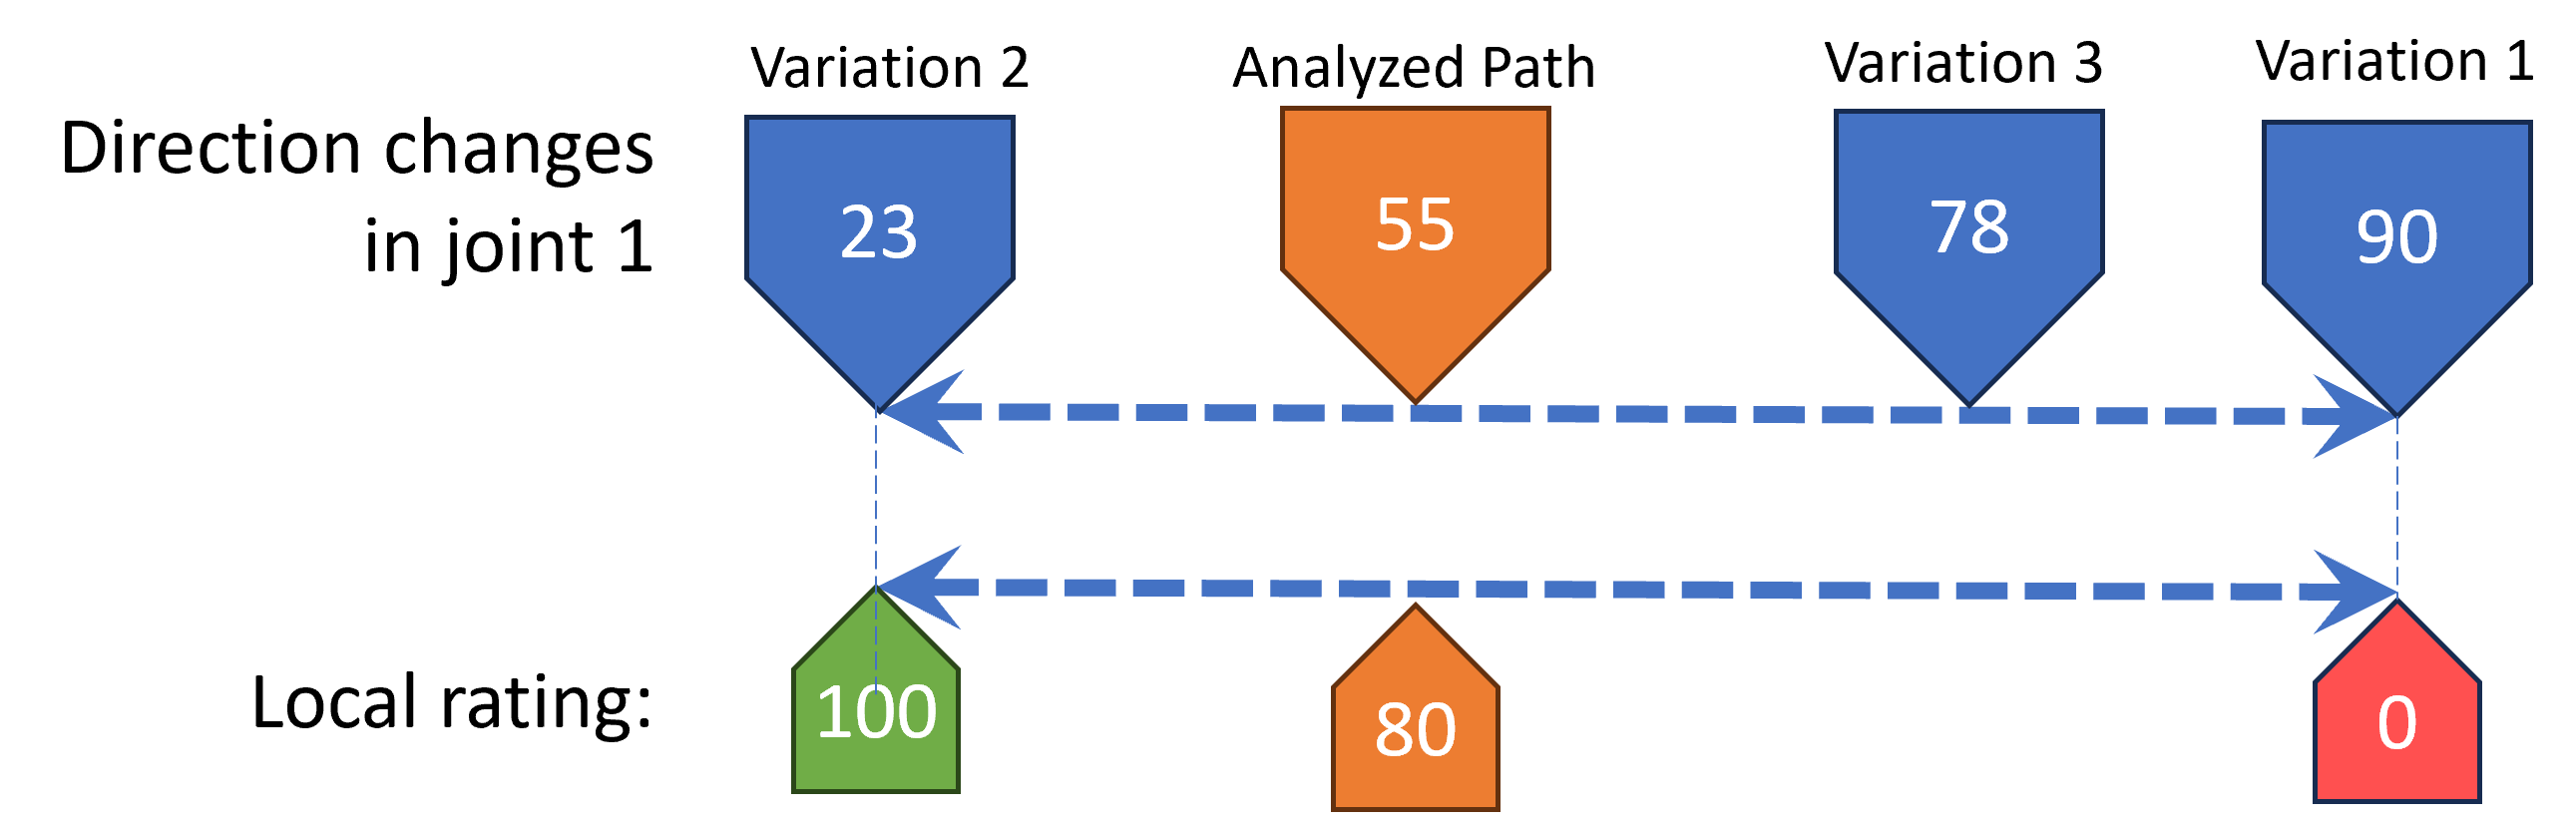
\includegraphics[width=0.8\textwidth]{figures/localscore.png}}
	\caption{Calculation of the local score trough variation}
	\label{Localscore}
\end{figure}

It is important to note that performing more variations before calculating the local sore will increase the accuracy of this approach. If only a few variations are performed, it is possible that only variations with similar outcomes will be found, which can skew the result significantly.

Another factor that needs to be analyzed is whether the variations in the boundary result in local scores that exceed a certain standard deviation. Figure \ref{lowstd}, shows how a local score of 66 is calculated despite the presence of very small absolute differences. In this case, the standard deviation is only 0.37. Figure \ref{highstd} demonstrates how the same local score of 66 is calculated even though the absolute differences are significantly higher. Here, the standard deviation is 22.36. Only if the standard deviation exceeds a set threshold should the local score be used as input for the global score. In cases where the standard deviation criteria is not met, the corresponding process parameter should be omitted from the global score calculation.

\begin{figure}[H]
	\centerline{\includegraphics[width=0.8\textwidth]{figures/lowstd.png}}
	\caption{Variation with low standard deviation}
	\label{lowstd}
\end{figure}

\begin{figure}[H]
	\centerline{
\includegraphics[width=0.8\textwidth]{figures/highstd.png}}
	\caption{Variation with high standard deviation}
	\label{highstd}
\end{figure}

 
\subsection{Information Extraction form Time-Series Data}\label{extraction}
It is important to note that for a local score computation, as mentioned in Chapter \ref{LRC}, a time-series needs to be transformed into a scalar value. This can either be done by directly transforming the time-series like, for example, summing up all values or performing a subsequent analysis. As each time-series is capturing different physical phenomena, each one requires an individual process for transforming into a scalar value.
\newpage




\section{Information from Angular Position}
In its isolated form, the angular position of a joint does not provide information to enable extensive qualitative analysis. However, when supplemented with temporal information, it becomes a valuable source of information. By considering the angular position in conjunction with the temporal dimension, a more comprehensive understanding of joint behavior can be obtained, allowing for more in depth analysis.



Figure \ref{agularstuff} visualizes what information needs to be added to enrich the analysis of these process parameters that are directly related to the angular position of joints.

\begin{figure}[H]
	\centerline{\includegraphics[width=0.8\textwidth]{figures/angularstuff.png}}
	\caption{Additional Information for angular position of each joint}
	\label{agularstuff}
\end{figure}



The first additional piece of required information is the temporal element, which specifies the specific time at which a joint should be in a particular rotational position. This information can be recorded in equidistant time steps, as shown in figure \ref{equi} on the left, or it can be adapted to only record the change in position, as shown on the right. However, recording only the change in position is not ideal because it does not accurately represent the physical system, where the position cannot change significantly from one time step to the next. Moreover, this method does not specify the rotational velocity at which the joint should change position. On the other hand, continuous recording in small equidistant time steps can result in a larger number of recorded values and, consequently, a longer time-series.

Figure \ref{equi} illustrates the rotational position of a rotary joint in radians. The left side of the figure displays the position recorded with equidistant time steps, while the right side shows a time-series where only the destination positions and their corresponding times are recorded.


\begin{figure}[H]
	\centerline{
\includegraphics[width=1\textwidth]{figures/equionchange.png}}
	%\caption{Time-series of a rotary joint with equidistant time steps}
	\caption{Two option for recording the joint position in a time-series}
	\label{equi}
\end{figure}

%\begin{figure}[H]
%	\centerline{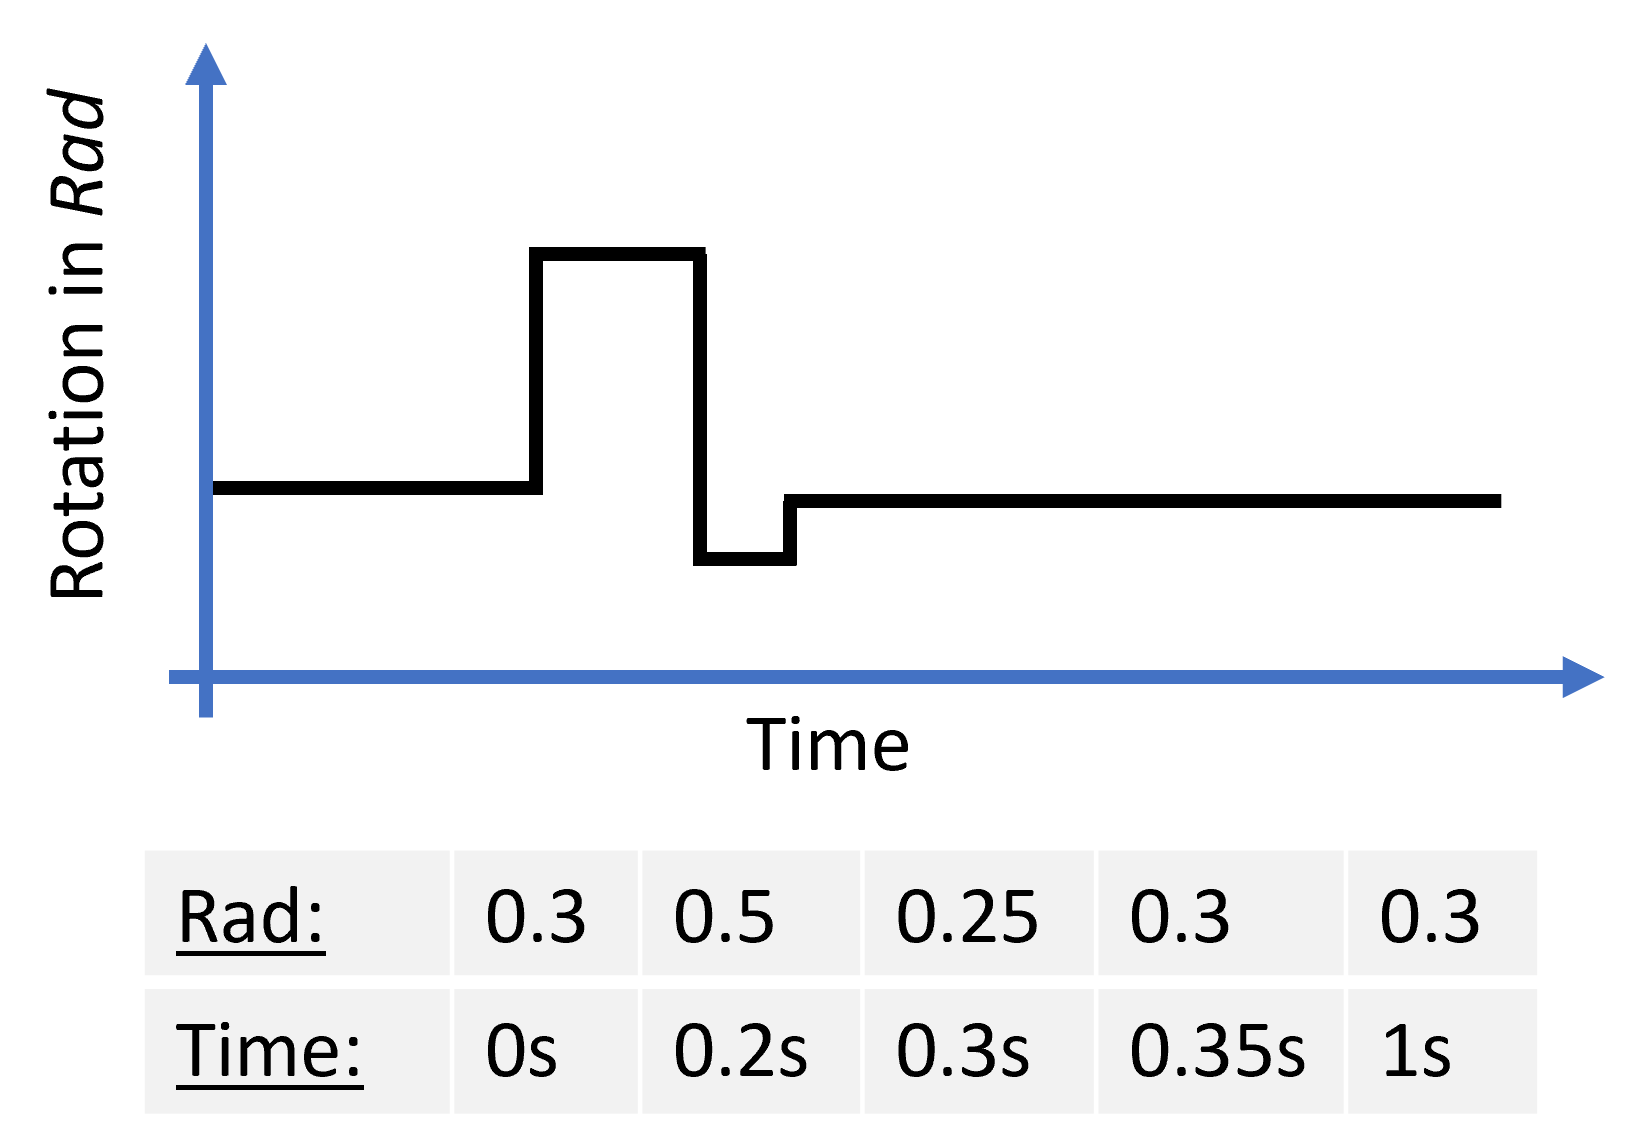
\includegraphics[width=0.5\textwidth]{figures/onchange.png}}
%	\caption{Time-series of a rotary joint with only the recorded end positions}
%	\label{onchange}
%\end{figure}

\subsection{Total Joint Travel and Direction Changes}
Parameters that can be analyzed without requiring any additional information include the number of direction changes and the total travel of a joint. The total travel can be determined by subtracting the position of two adjacent recorded points and summing up the absolute values. Furthermore, additional information can be extracted by separately summing up the clockwise and anti-clockwise rotations. By combining the absolute values of these rotations, the total travel of the joint can be calculated.

igure \ref{travel} provides a visual representation of the calculation of total travel. The total forward rotation can be obtained by summing up the lengths of the green arrows, while the total backward rotation is determined by summing up the lengths of the orange arrows.

\begin{figure}[H]
	\centerline{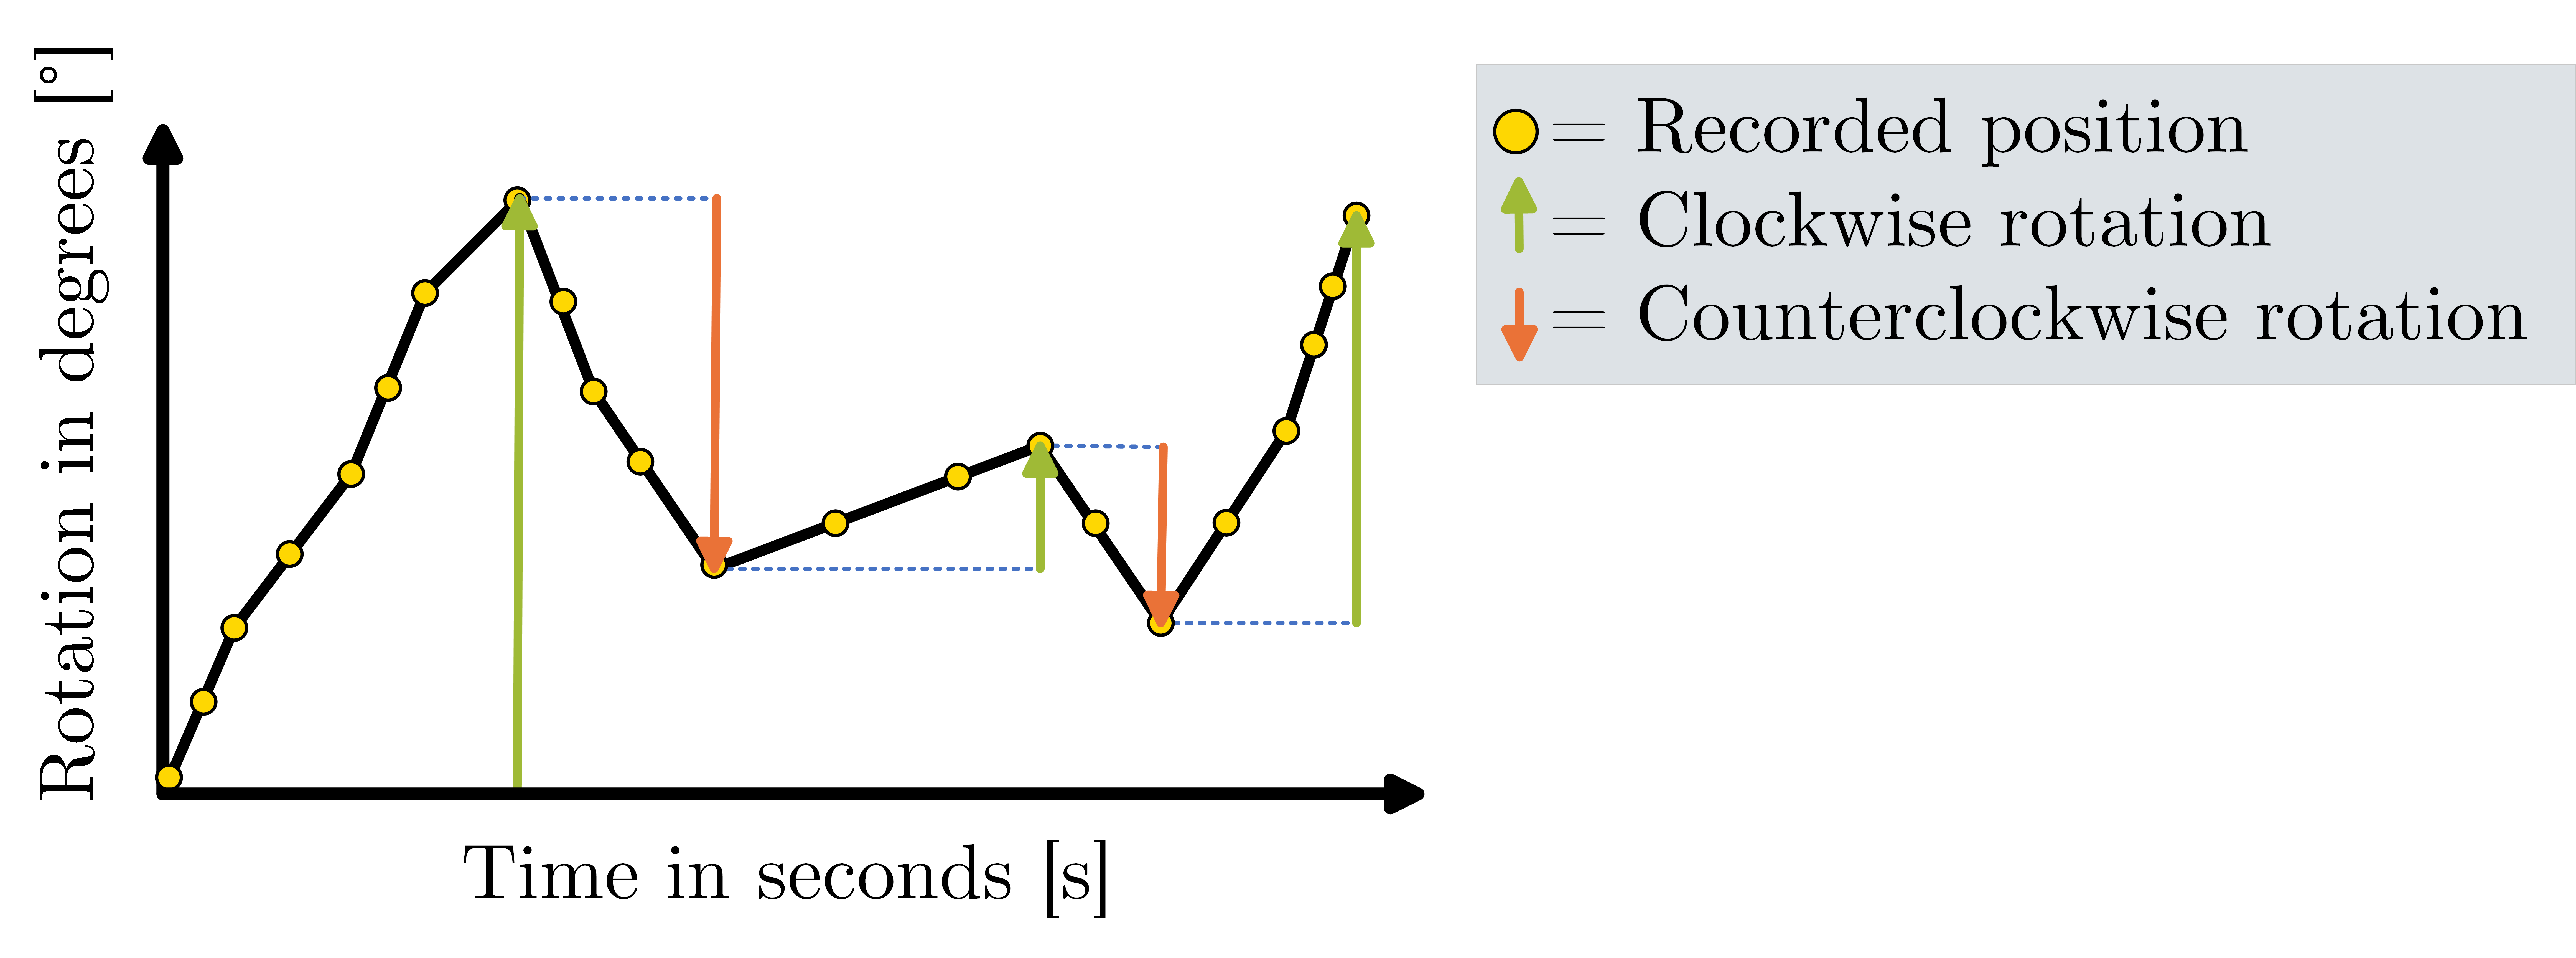
\includegraphics[width=0.5\textwidth]{figures/travel.png}}
	\caption{Summing up the rotation in the clockwise and anti-clockwise direction }
	\label{travel}
\end{figure}

The number of direction changes is a parameter that can be determined by analyzing the joint position alone, without the need for temporal information. This can be done by identifying all points where the position before and after is either smaller or larger. However, it is important to note that this method may not be applicable to points where multiple positions are recorded at the same value right after each other.

To address the issue of multiple positions recorded at the same value, a possible solution is to introduce a tracking value that indicates whether the previous change in direction of two adjacent positions was either up or down. If the direction of two positions is different from the tracking value, the direction change counter is incremented by 1. However, if the direction is the same as the previous points or if the positions are identical (neutral), the direction change counter and tracking values remain unchanged.

Figure \ref{dirchange} gives a visual representation of where the direction-change-counter is incremented.

\begin{figure}[H]
	\centerline{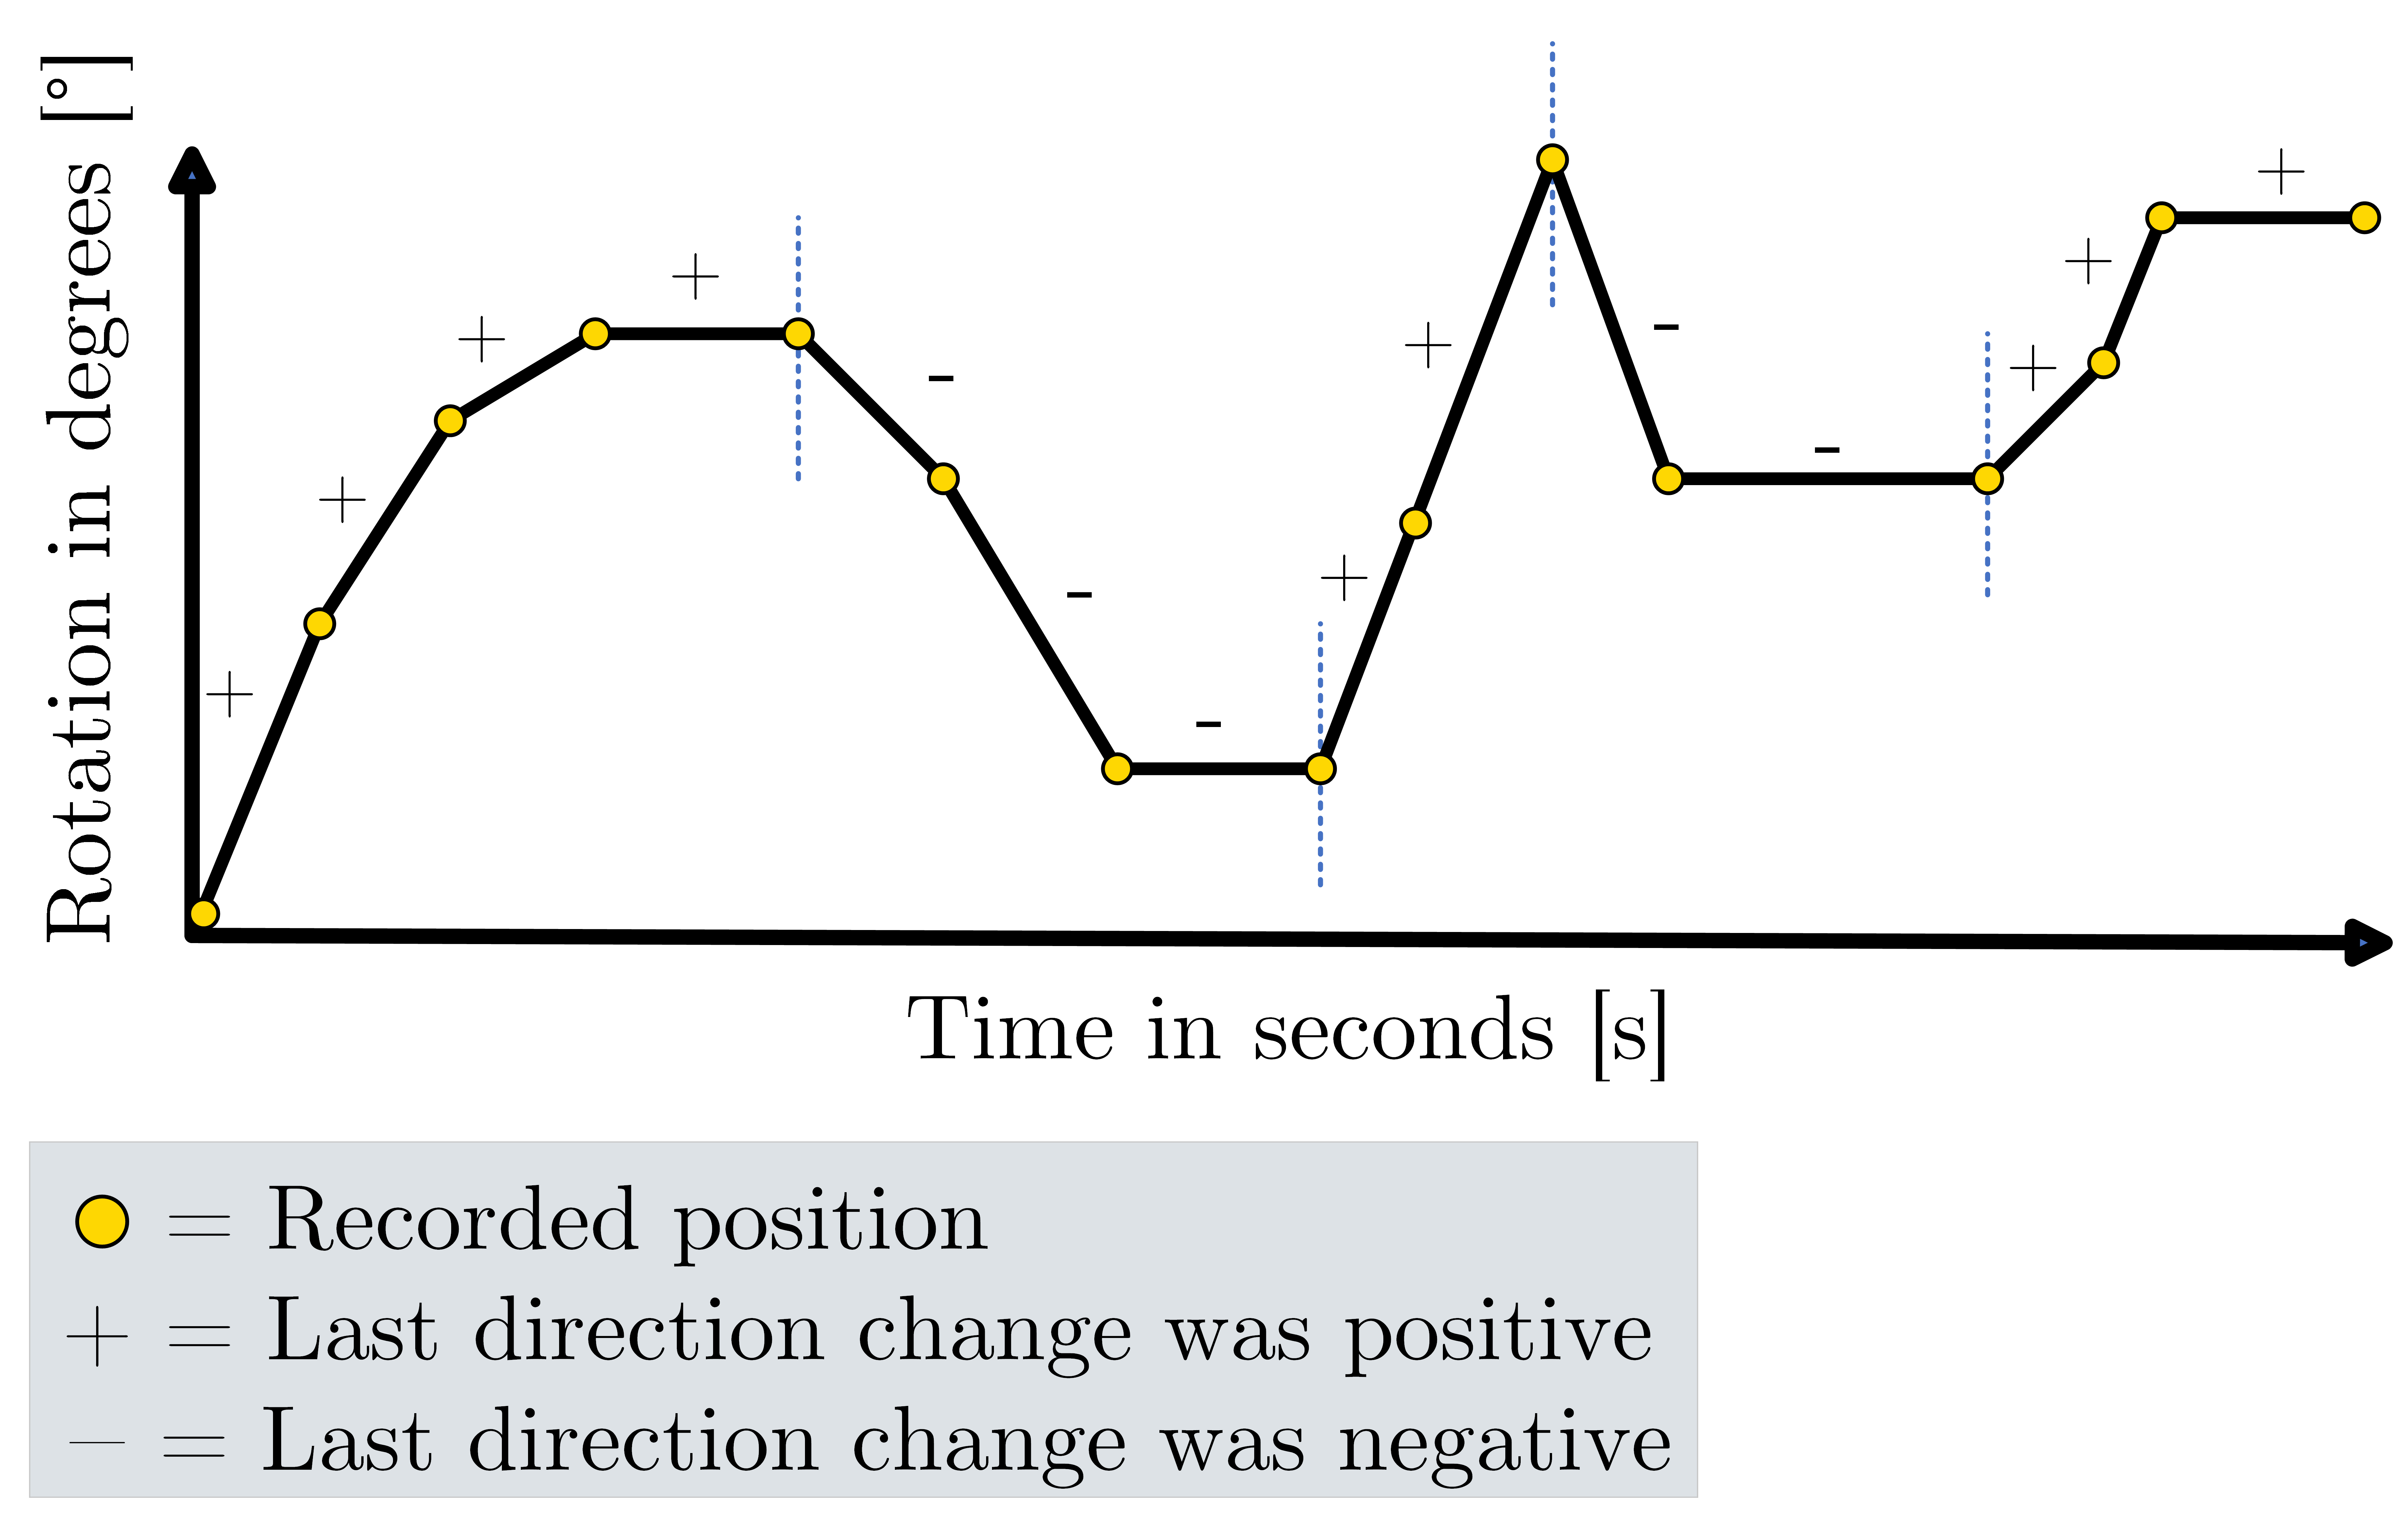
\includegraphics[width=0.8\textwidth]{figures/dirchange.png}}
	\caption{Calculating direction changes from a time-series}
	\label{dirchange}
\end{figure}

The counters for direction changes and total travel of each joint can be transformed into a local score, as explained in Chapter \ref{LRC}. This local score can then be multiplied by an importance factor to calculate the overall local score. The direction changes can be summed up over all joints, or they can be specifically grouped based on certain criteria or categories.  

Table \ref{exampleDirTravel} gives an example of how a global score can be calculated based only on the number of direction changes and total travel. This table demonstrates how different joints and parameters can be weighted and grouped together to calculate the global score. By assigning different importance factors to each parameter, the overall global score can reflect the desired outcome. It is important to note that only the local scores are multiplied by the importance factor, not the actual counted direction changes or total travel values. This allows the local score to fall within the range of 0 to 100. In this example, due to the high local score and importance factor for the direction changes in joint 1, the overall global score is also very high, indicating its significance in the calculation.


\begin{table}[H]
	\centering
	\begin{tabular}{||l|r|r|r||}
		Process Parameters & Local rating & Importance & Local score\\
		\hline
		\hline
		\hline
		
		Direction changes in joint 1 & 95 & 0.7 & 66.5\\
		Direction changes in joint 2-6 & 45& 0.1&4.5\\
		Total travel in joint 4& 34& 0.1&3.4\\
		Total travel in joint 1-3 and 5-6& 46&0.1&4.6\\
		\hline
		\hline
		\hline
		Global Score& & &79\\
		\hline
		\hline
	\end{tabular}
	
	\caption{Calculation of a score regarding only direction changes and total travel}
	\label{exampleDirTravel}
\end{table}

In certain cases, it may not be possible to reduce the number of direction changes by adjusting the boundary conditions. It is important to note that having the same number of direction changes does not imply that two time-series are identical. Figure \ref{dirchangeSTD} provides a visual representation of two time-series with the same number of direction changes but distinct characteristics.

To distinguish between these cases, the standard deviation can be utilized. By incorporating the standard deviation, tool paths that result in frequent and closely spaced direction changes can be identified and generally considered less desirable.

To combine the factor of standard deviation with the number of direction changes, they can be integrated into a single parameter. This is achieved by dividing the number of direction changes by the standard deviation. By incorporating this variation-based calculation, a local score can be determined.

When there are only a few direction changes but with a high variance, the resulting parameter value will be low. Conversely, when there are numerous direction changes but with a low variance, the parameter value will be high.

This approach provides a evaluation method that considers both the quantity of direction changes and the variability within the time-series data.

\begin{figure}[H]
	\centerline{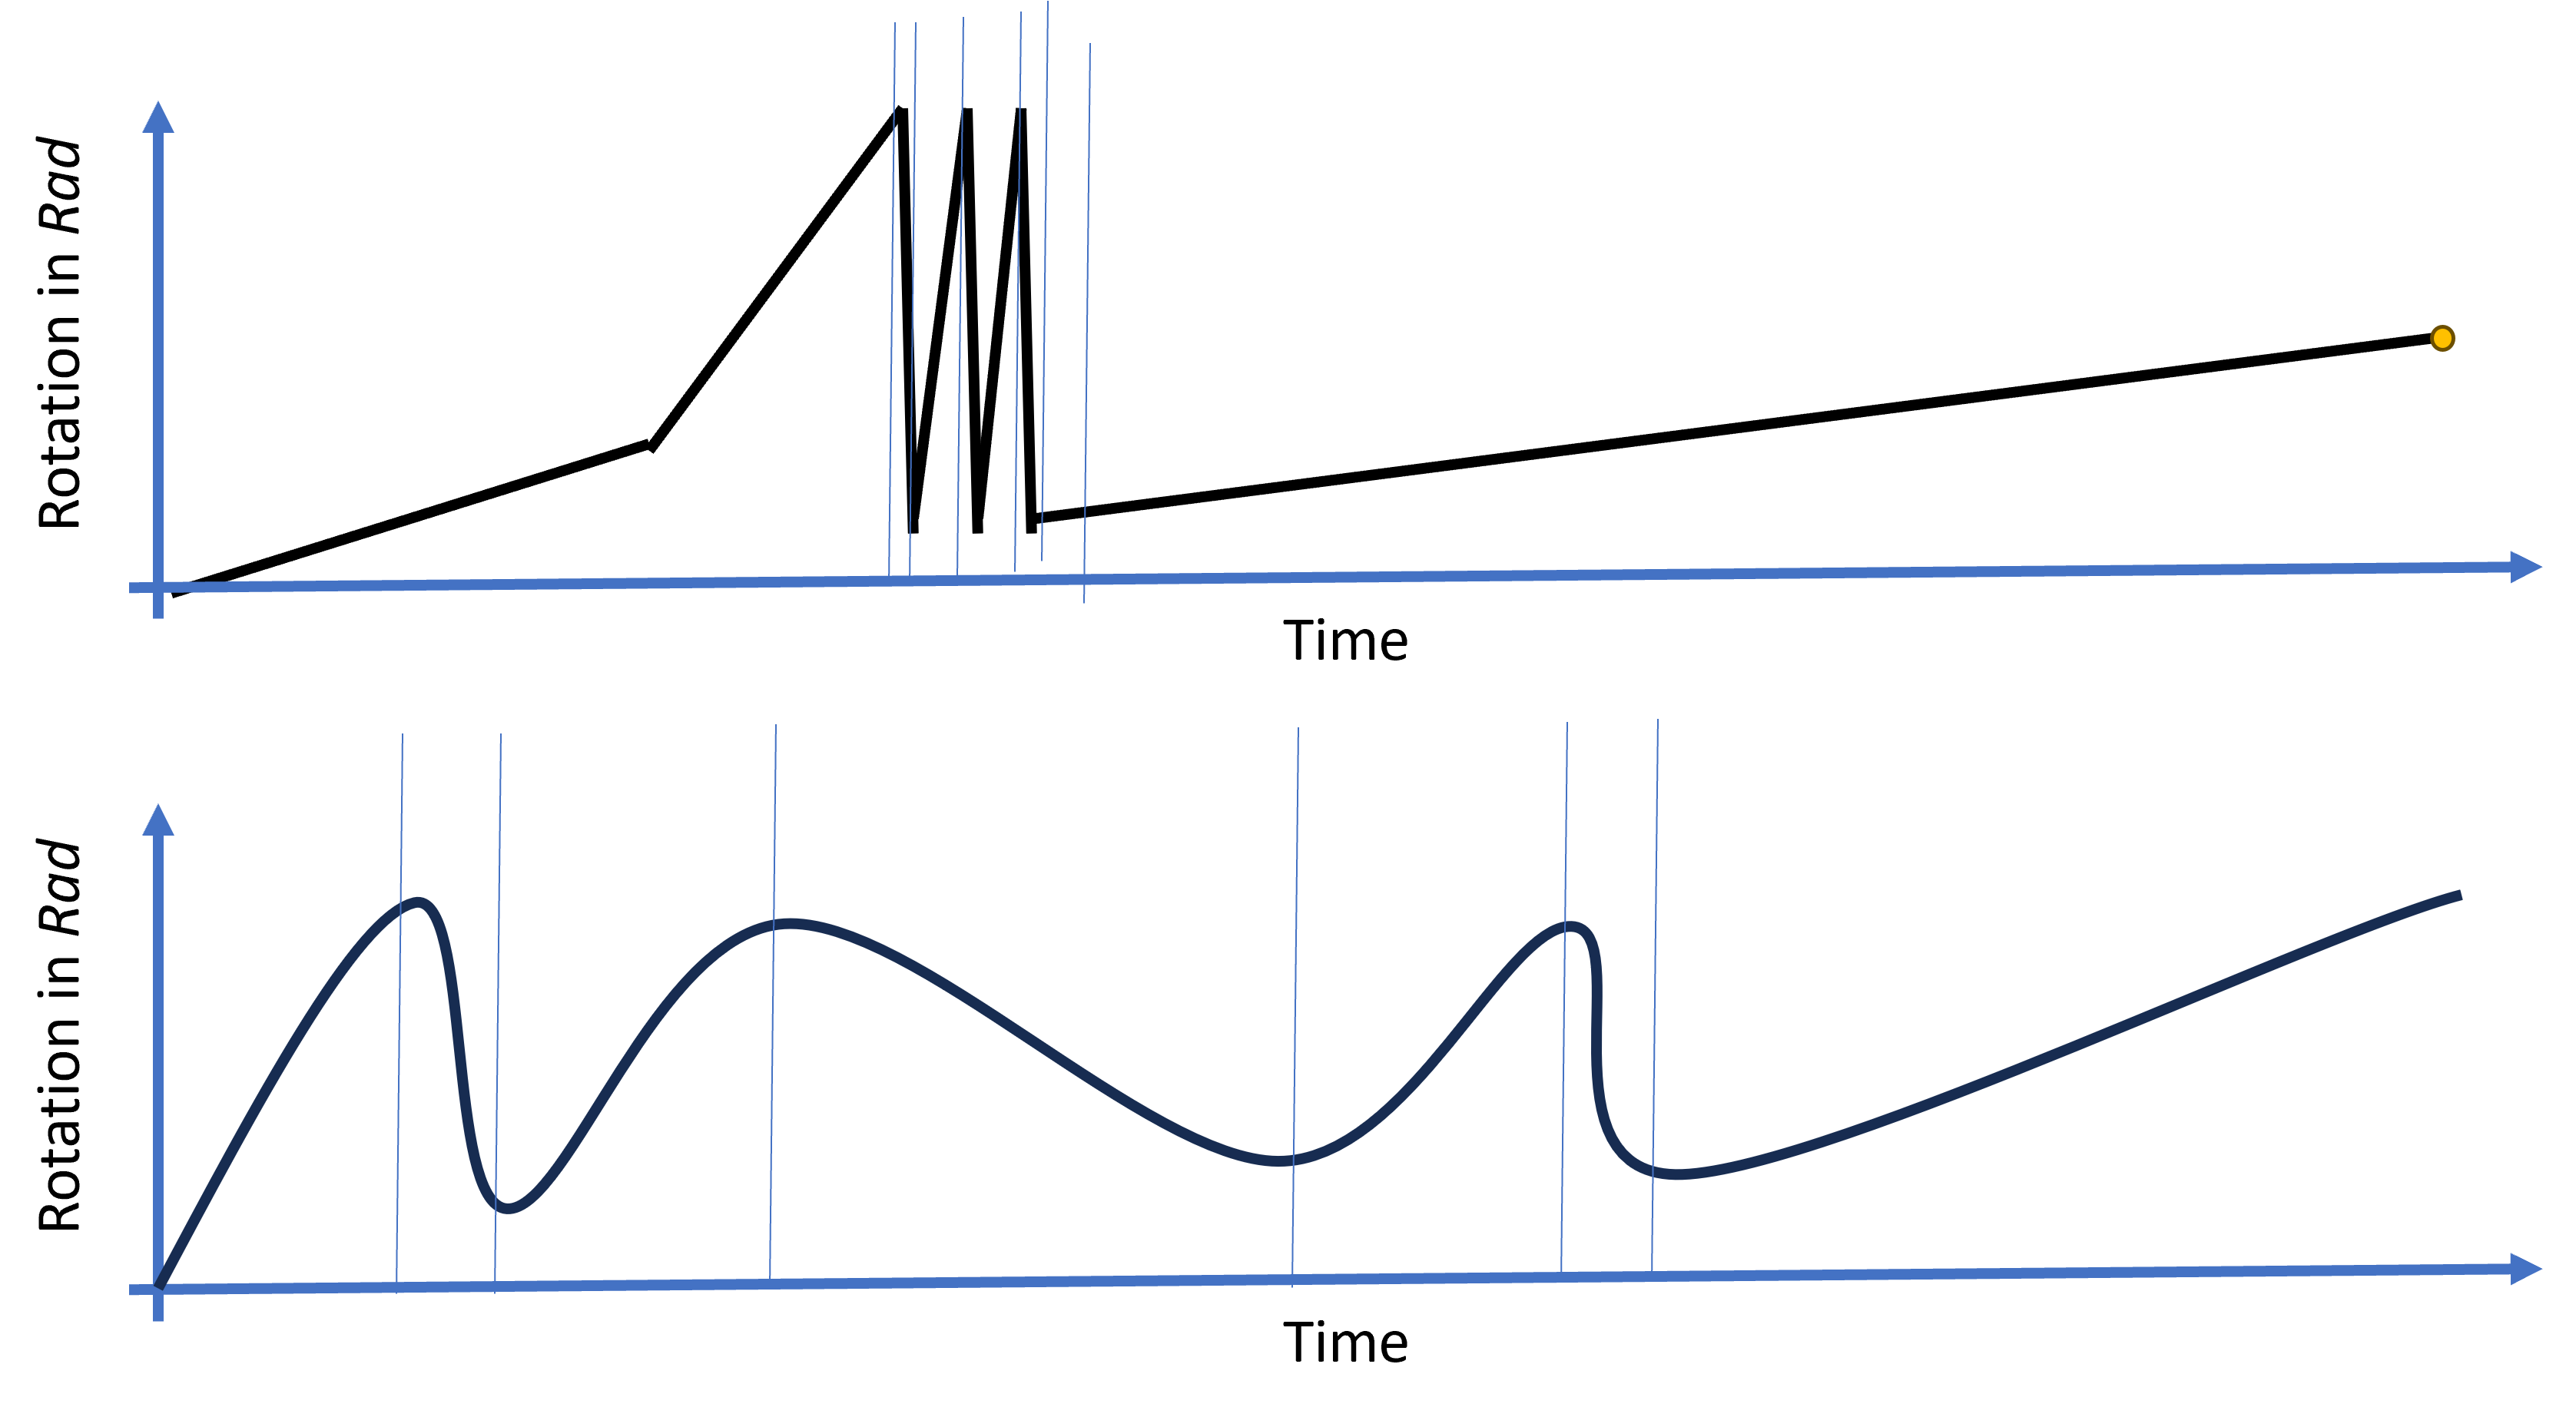
\includegraphics[width=0.7\textwidth]{figures/DirSTD.png}}
	\caption{Two Time-Series with equal number of direction changes but different characteristics}
	\label{dirchangeSTD}
\end{figure}

\subsection{Rotation Limits}\label{RotLim}
In addition, a straightforward analysis of the rotational limits can be conducted, requiring knowledge of two distinct values. The first value are the physical limit that a joint cannot surpass, as surpassing this limit can cause significant damage to the robot. The second value relates to potential soft limits in place to prevent over-rotation of the joint beyond its physical limits. To validate whether any rotational positions approach or exceed these limits, a simple comparison of all values can be performed. In cases where it is known that a joint is most stable within a specific range, additional limits can be defined accordingly.

Once a tool path with defined boundary conditions is established, the joint angles can be analyzed through a simple comparison process. If the joint positions surpass the soft limits or deviate excessively from the desired orientation, a "No-Go" exception is triggered. It's worth noting that the analysis of rotation limits does not contribute to the calculation of the global score but serves as a validity assessment to determine if the required movement for the tool path is physically feasible.
\newpage
\subsection{Velocity, Acceleration and Jerk of the Joints}\label{VAJJ}
To conduct a specific analysis of the rotational velocity, acceleration, and jerk of the joints, a time derivative needs to be applied. By performing simple comparisons of the time-series values, it becomes possible to determine whether the maximum capabilities of the motor driving the joint are being exceeded.

Figure \ref{velo} demonstrates how the velocity aspect can be transformed into a scalar value, which can then be utilized in the calculation of a local score. Firstly, the joint velocity is obtained by taking the time derivative of the joint position. Subsequently, an analysis is conducted to determine the duration for which the absolute velocity exceeds a certain threshold value. In the given example, the threshold is set at 80\%. Additionally, it is feasible to incorporate multiple thresholds and assign exponential weights to them relative to each other. The combined outcome is then utilized to calculate the local score.

\begin{figure}[H]
	\centerline{\includegraphics[width=1\textwidth]{figures/veloy.png}}
	\caption{Calculating velocity from the joint position over time}
	\label{velo}
\end{figure}

It is also possible to define if a short but significant peak over the threshold values is more desirable than a constant but small overstep. Figure \ref{peaklong} gives a visualization of these two cases. In the former case, where peaks are more desirable, it is enough to sum up The area between the velocity and set threshold. If the avoidance peaks is the first priority, all elements in the velocity time series can be cubed and summed up. By cubing the values, peaks will be weight exponentially and thus easier to optimize for.

\begin{figure}[H]
	\centerline{
\includegraphics[width=1\textwidth]{figures/peaklong.png}}
	\caption{Overstepping the threshold value}
	\label{peaklong}
\end{figure}


The simplest case, however, is to square all values and sum them. By employing this method, there is no need to define threshold boundaries. Additionally, high peaks will have a greater influence on the resulting value compared to small constant values, without overshadowing the final result.

If the velocity exceeds the maximum velocity, an exception called "No-Go" must be thrown, indicating that the movement is not possible. The same rating principle can be applied to acceleration and jerk. The acceleration is obtained by taking the derivative of the velocity, while the jerk is obtained by taking the next derivative. Individual limits and thresholds can be set to determine the optimality of the robot's movement. If the maximum acceleration or jerk is exceeded, a "No-Go" error is also thrown.


Table \ref{VAJ} presents the calculation of a global score, which incorporates a weighting that prioritizes low acceleration in joint 2 and allows for high velocity in all joints. The acceleration in joint 1 and joints 3 to 6 are considered to be of lesser significance. The jerk is completely omitted from the rating in this example.


\begin{table}[H]
	\centering
	\begin{tabular}{||l|r|r|r||}
		Process Parameters & Local rating & Importance & Local score\\
		\hline
		\hline
		\hline
		Velocity in Joints 1-6& 45& 0.1&4.5\\
		Accelerations in Joint 2& 90 & 0.8 & 72\\
		Accelerations in Joint 1 and 3-6 & 15& 0.1&1.5\\
		Jerk in joints 1-6& 4& 0&0\\
		
		\hline
		\hline
		\hline
		Global Score& & &78\\
		\hline
		\hline
	\end{tabular}
	
	\caption{Calculation of a score regarding only velocity, acceleration and jerk}
	\label{VAJ}
\end{table}


\section{TCP Coordinates, Velocity and Acceleration}\label{CVA}
As discussed in Chapter \ref{pp}, the forward kinematics approach allows for the calculation of the TCP's X-Y-Z coordinates and orientation. Alternatively, this information can be directly extracted from the G-code.

By calculating the time derivative of the positions, it is possible to determine both the velocity and acceleration of the TCP. These parameters play a significant role in milling applications, particularly when precise corners need to be fabricated. It is important to note that both robotic systems and CNC machines have limitations on their acceleration capabilities. As highlighted in Chapter \ref{CPM}, these limitations result in slight deviations occurring in the path, especially at corners. These deviations arise from the systems' inability to instantaneously change velocity or direction. Consequently, the TCP's path will not be perfectly followed as demanded by the G-Code and will exhibit minor variations in the corners.

To quantitatively analyze the magnitude and frequency of these deviations, it is crucial to examine the endpoints of the linear toolpath as defined in the G-code. When the endpoints are aligned along a vector in space, it indicates that no deviation from the desired toolpath is expected. However, a misalignment between the endpoints suggests an anticipated deviation.

Figure \ref{devi} gives a visual example of the position in th X-Y plane that the robot needs to traverse. The expected deviation is shown in red.

\begin{figure}[H]
	\centerline{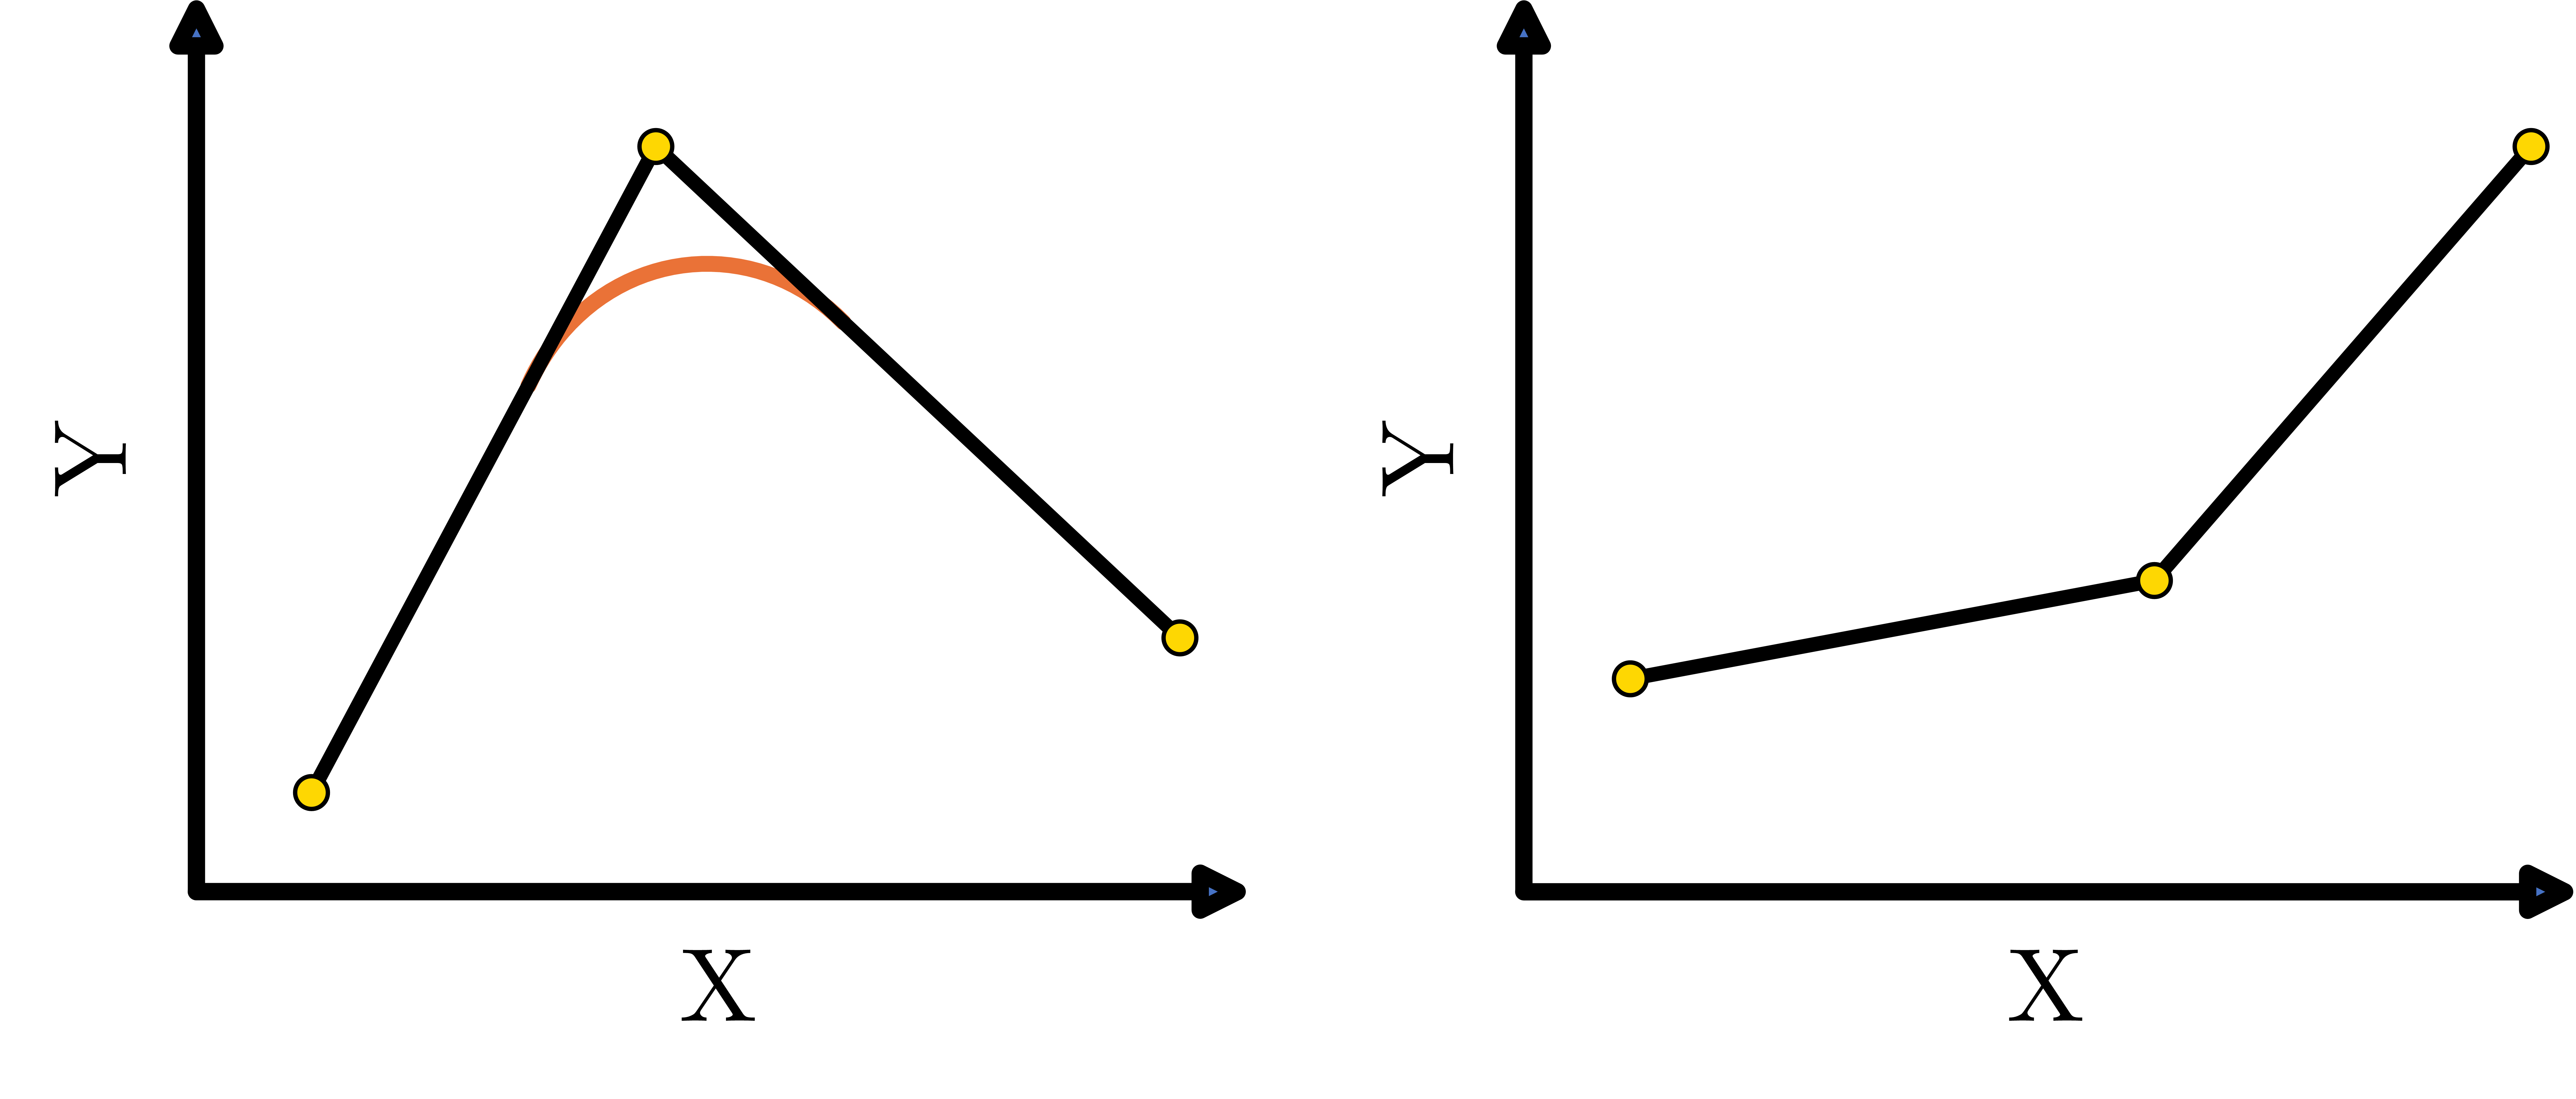
\includegraphics[width=.651\textwidth]{figures/uber.png}}
	\caption{Deviation of of the TCP from the actual toolpath}
	\label{devi}
\end{figure}

In order to obtain a qualitative estimate of the total deviation, it is necessary to analyze the individual velocity vectors that characterize the toolpath. Perfect alignment of the velocity vectors indicates no expected deviation. However, as the angle between consecutive velocity vectors increases, the deviation also increases.

To quantitatively represent this information, the sine of each angle can be calculated and summed. An angle of 0 or 180 degrees will result in a value of 0, while an angle of 90 degrees will yield a value of 1. This scalar value provides an indication of the overall magnitude of the expected deviation.

Additionally, it is crucial to consider the magnitude or speed of the velocity vectors. In cases involving sharp corners with high velocities, the deviation is anticipated to be more significant compared to corners with lower velocities. To account for this, the result obtained from the sine calculation can be multiplied by the smaller of the two velocities.

This analysis is useful for operators in defining more optimal machining strategies. However, it is important to note that this analysis is separate from the optimization involving the redundant DoF.

In the context of WAAM, the acceleration of the welding torch plays a crucial role in the process. This is particularly evident when utilizing CMT technology, which involves wire retraction, as discussed in Chapter \ref{CMT}. A rapid acceleration of the welding torch can lead to unintended drop detachment and imprecise drop placement. Consequently, the quality and accuracy of the additive manufacturing process may be compromised, resulting in defects and deviations from the desired geometry.

However, it is worth noting that, similar to the deviation in the toolpath discussed earlier, this issue cannot be directly optimized by simply defining specific boundary conditions.

\section{Energy Usage}
Energy usage is a crucial aspect of modern manufacturing. To minimize unnecessary and energy-intensive movements, it is essential to select appropriate boundary conditions for robots. The analysis of energy usage can be approached in two distinct ways. Firstly, a continuous energy analysis allows to attribute specific energy consumption to each movement. Secondly, it is possible to consider the overall energy requirement throughout the entire manufacturing process, providing a holistic perspective on energy utilization. These approaches can optimize energy usage and make informed decisions regarding energy efficiency in manufacturing. 

\subsection{Continuous Energy-Usage}
Tracking energy consumption can be achieved through a straightforward method of monitoring the velocity and acceleration of individual joints. The energy demand is composed of two components: the rotational movement of a joint at a predetermined speed and the joint's acceleration.

To determine the energy consumed by each joint, the time-series data of joint velocity can be multiplied by the average energy consumption value associated with that particular joint. The same principle is applied to the time-series data of joint acceleration. By summing up these resultant time-series, an energy consumption profile for each joint can be obtained. Aggregating the time-series data from all joints provides an overall estimation of the robot's energy consumption. Table \ref{scalers} gives exemplary values for the scaling factors.\newline


\begin{table}[H]
	\centering
	\begin{tabular}{||l|r|r||}
		Joint Nr.  & Velocity Scaling in \(\frac{\si[per-mode=symbol]{\kWh}}{\si[per-mode=symbol]{\m\per\sec }}\)& Acceleration Scaling in \(\frac{\si[per-mode=symbol]{\kWh}}{\si[per-mode=symbol]{\m\per\sec\squared }}\) \\
		\hline
		\hline
		\hline
		Joint 1	& 0.1 & 0.5\\
		Joint 2	&  0.4& 0.3 \\
		Joint 3	& 0.3& 0.2\\
		...& ...& ...\\
		
		\hline
		\hline
	\end{tabular}
	
	\caption{Average scaling factors for energy calculations}
	\label{scalers}
\end{table}


This approach offers a notable advantage in its simplicity. Nevertheless, its primary limitation stems from the potential inaccuracies that may arise when working with an average scaling value. If this value is derived by averaging all possible positions, but only a limited number of positions are actually traversed by the robot, significant discrepancies can occur.


To address these limitations, more advanced approaches are necessary. For instance, the utilization of multi-body simulations in CAM software enables a direct analysis of the exact energy requirements for a robot to move between different poses. This method involves precise modeling of weight distribution, resulting in highly accurate outcomes. However, it is important to consider that implementing this approach may require substantial computation and development time.


Another viable option to consider is the utilization of a machine learning (ML) approach for estimating energy consumption during transitions between discrete poses. By employing a supervised learning technique, where the input data includes the current pose (joint positions and velocities) as well as the target pose, an ML model can be trained to predict the energy required for each transition. This approach offers the advantage of leveraging ML algorithms to provide accurate energy consumption estimates in a more efficient manner. However, it is important to acknowledge that generating high-quality training data and training the ML model can be time-intensive processes.

Figure \ref{ENERGYOPTIONS} illustrates the three aforementioned options along with their key requirements. It is important to note that these examples only give an example on how to get a energy estimation and do not cover all possible solutions to address this problem. 

\begin{figure}[H]
	\centerline{\includegraphics[width=.8\textwidth]{figures/ENERGYOPTIONS.png}}
	\caption{Exemplary methods for energy usage calculations}
	\label{ENERGYOPTIONS}
\end{figure}

Once the time-series data for energy consumption is obtained, it becomes possible to identify peaks and associate them with specific movements. In line with the optimization objective, it is also feasible to establish threshold values, as discussed in Chapter \ref{CVA}, to optimize for a consistent energy consumption.


\subsection{Total Energy-Usage}
When the aim is to obtain a single scalar value for energy consumption, the same procedures outlined in the preceding chapter can be applied, and the values from the time series can be aggregated through summation.

In situations where the temporal information in energy consumption is considered irrelevant, alternative machine learning approaches can be employed. For example, Recurrent Neural Networks (RNNs) can be utilized, as they have the ability to take an entire time series as input and generate a scalar value representing the total energy consumption. RNNs excel at capturing dependencies and patterns in sequential data. By training an RNN model using a time series dataset, it can learn to predict the total energy consumption based on the provided input. However, it is important to note that, like most machine learning approaches, this method requires substantial effort and time for generating training data and conducting the training process.

In WAAM, it is important to consider the energy consumption associated with the welding process itself. The determination of energy use in welding involves various factors. The G-code, which comprises instructions for the welding process, can provide information on the movement, voltage and the desired power input. By analyzing this code, it becomes possible to estimate the energy consumption during each welding operation. Alternatively, these parameters are often pre-defined as constants on the welding appliance, with the G-code solely specifying the turn-on and turn-off points.

In addition to the factors mentioned earlier, the duration of the welding process and the parameters of the welding equipment play crucial roles in determining energy consumption. By considering these factors, it is possible to accurately assess the energy usage during welding operations.

However, this specific part of the total energy consumption cannot be optimized by defining the boundary conditions of redundant DoFs. The energy required for the welding process is solely defined by the welding parameters and G-code.


\section{Reach, Singularities and Torch Orientation}
The following discusses the robot poses with respect to reach, singularity avoidance, and torch orientation. These factors are essential in ensuring successful and efficient robotic operations.
\subsection{Reach and Orientation}\label{RO}

As mentioned in Chapter \ref{pp}, the analysis of the reachability index can be conducted in various formats. The first format involves a simple analysis to determine if all the points that the robot needs to traverse lie within its work volume, without any self-collisions or exceeding the hard joint limits. This aspect is closely related to the joint limits, as discussed in Chapter \ref{RotLim}. Additionally, it is necessary to analyze that there are no collisions between the robot and the workpiece. If all these parameters are met, a binary index can be used to indicate the feasibility and safety of executing the program. However, this index cannot be used for optimizing the robot's movement, as the parameters influencing this index are mostly defined by the G-Code.

When utilizing a robotic system with a specific tool, such as a milling spindle or a welding torch for WAAM, it is crucial to consider the boundary conditions associated with that tool. In many cases, the spindle and welding torch come with cables that provide power from an external power supply. These cables have an optimal orientation where bending and wear are minimized. By positioning the cables in an optimal orientation, the robotic system can operate efficiently and effectively without any interference or limitations due to cable movement, potential damage, or excessive bending or twisting.

Figure \ref{rot} illustrates the rotation around the C-axis of the welding torch, which leads to different strains on the wire with each rotation.

\begin{figure}[H]%
	\centering
	\subfloat[\centering No rotation]{{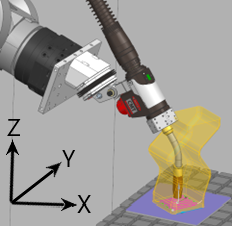
\includegraphics[width=.4\textwidth]{figures/rot0.png} }}%
	\qquad
	\subfloat[\centering 30 degree rotation]{{ 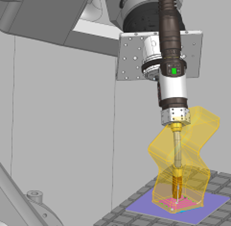
\includegraphics[width=.4\textwidth]{figures/rot1.png}}}%
	\caption{Rotation around the C-axis of a welding torch }%
	\label{rot}%
\end{figure}
 
To assess the efficiency of the robot's cable pose, it is important to consider additional parameters. In certain cases, it is preferable to route the cables in a specific orientation along a spatial vector, allowing for parallel translation or movement in the direction of that vector. In this case, the angle between the planes of the robot's base coordinate system remains constant.

Figure \ref{OOPti}a provides a visual representation of this example. The wire, shown in red, has an optimal orientation where the least amount of strain is present. Any position along that vector where the cable transitions to the welding torch tangentially is considered optimal. It is worth noting that this vector can be translated parallel in space while still maintaining its optimal status.

In certain scenarios, it is more efficient to route the cables towards a specific point in space, such as a mounting point on a wall. Figure \ref{OOPti}b illustrates an example where the optimal orientation of a milling spindle is directed towards a designated point where the cables originate. In this case, any position is considered optimal as long as the extended spindle vector aligns with the vanishing point.


\begin{figure}[H]%
	\centering
	\subfloat[\centering Optimal orientation along a vector ]{{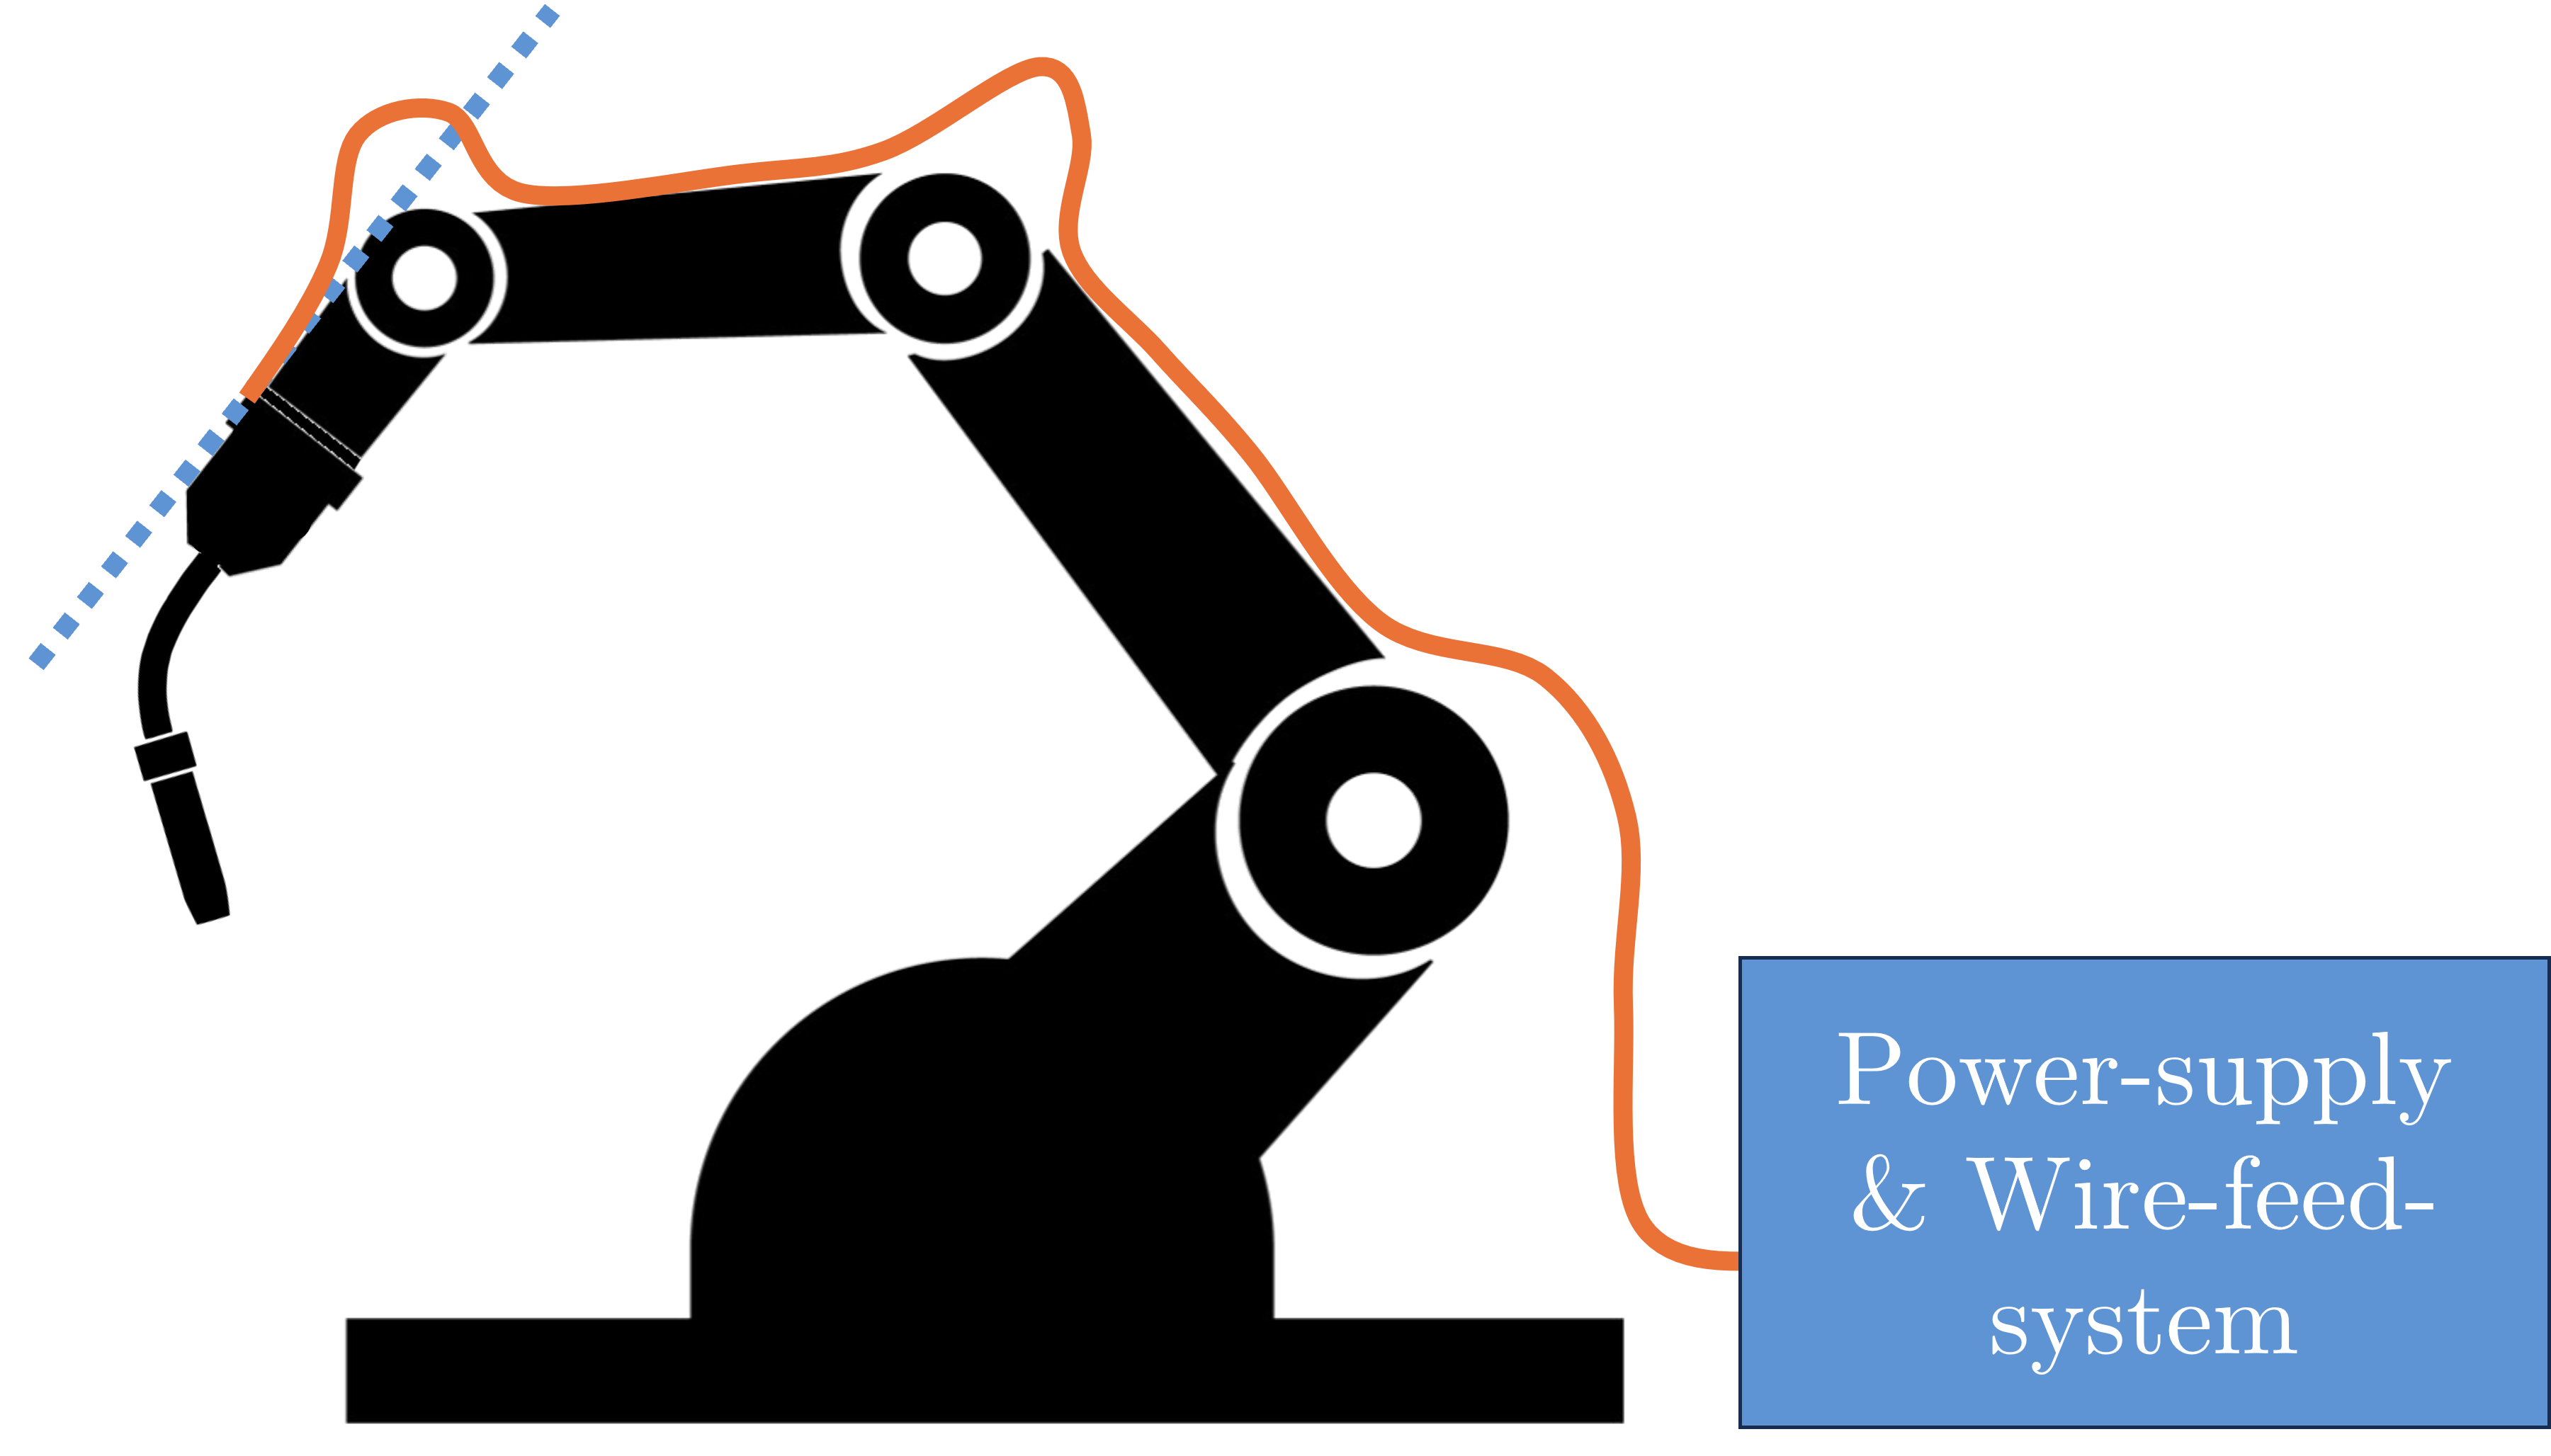
\includegraphics[width=.5\textwidth]{figures/paralell.png} }}%
	\qquad
	\subfloat[\centering Optimal orientation towards a defined points ]{{ 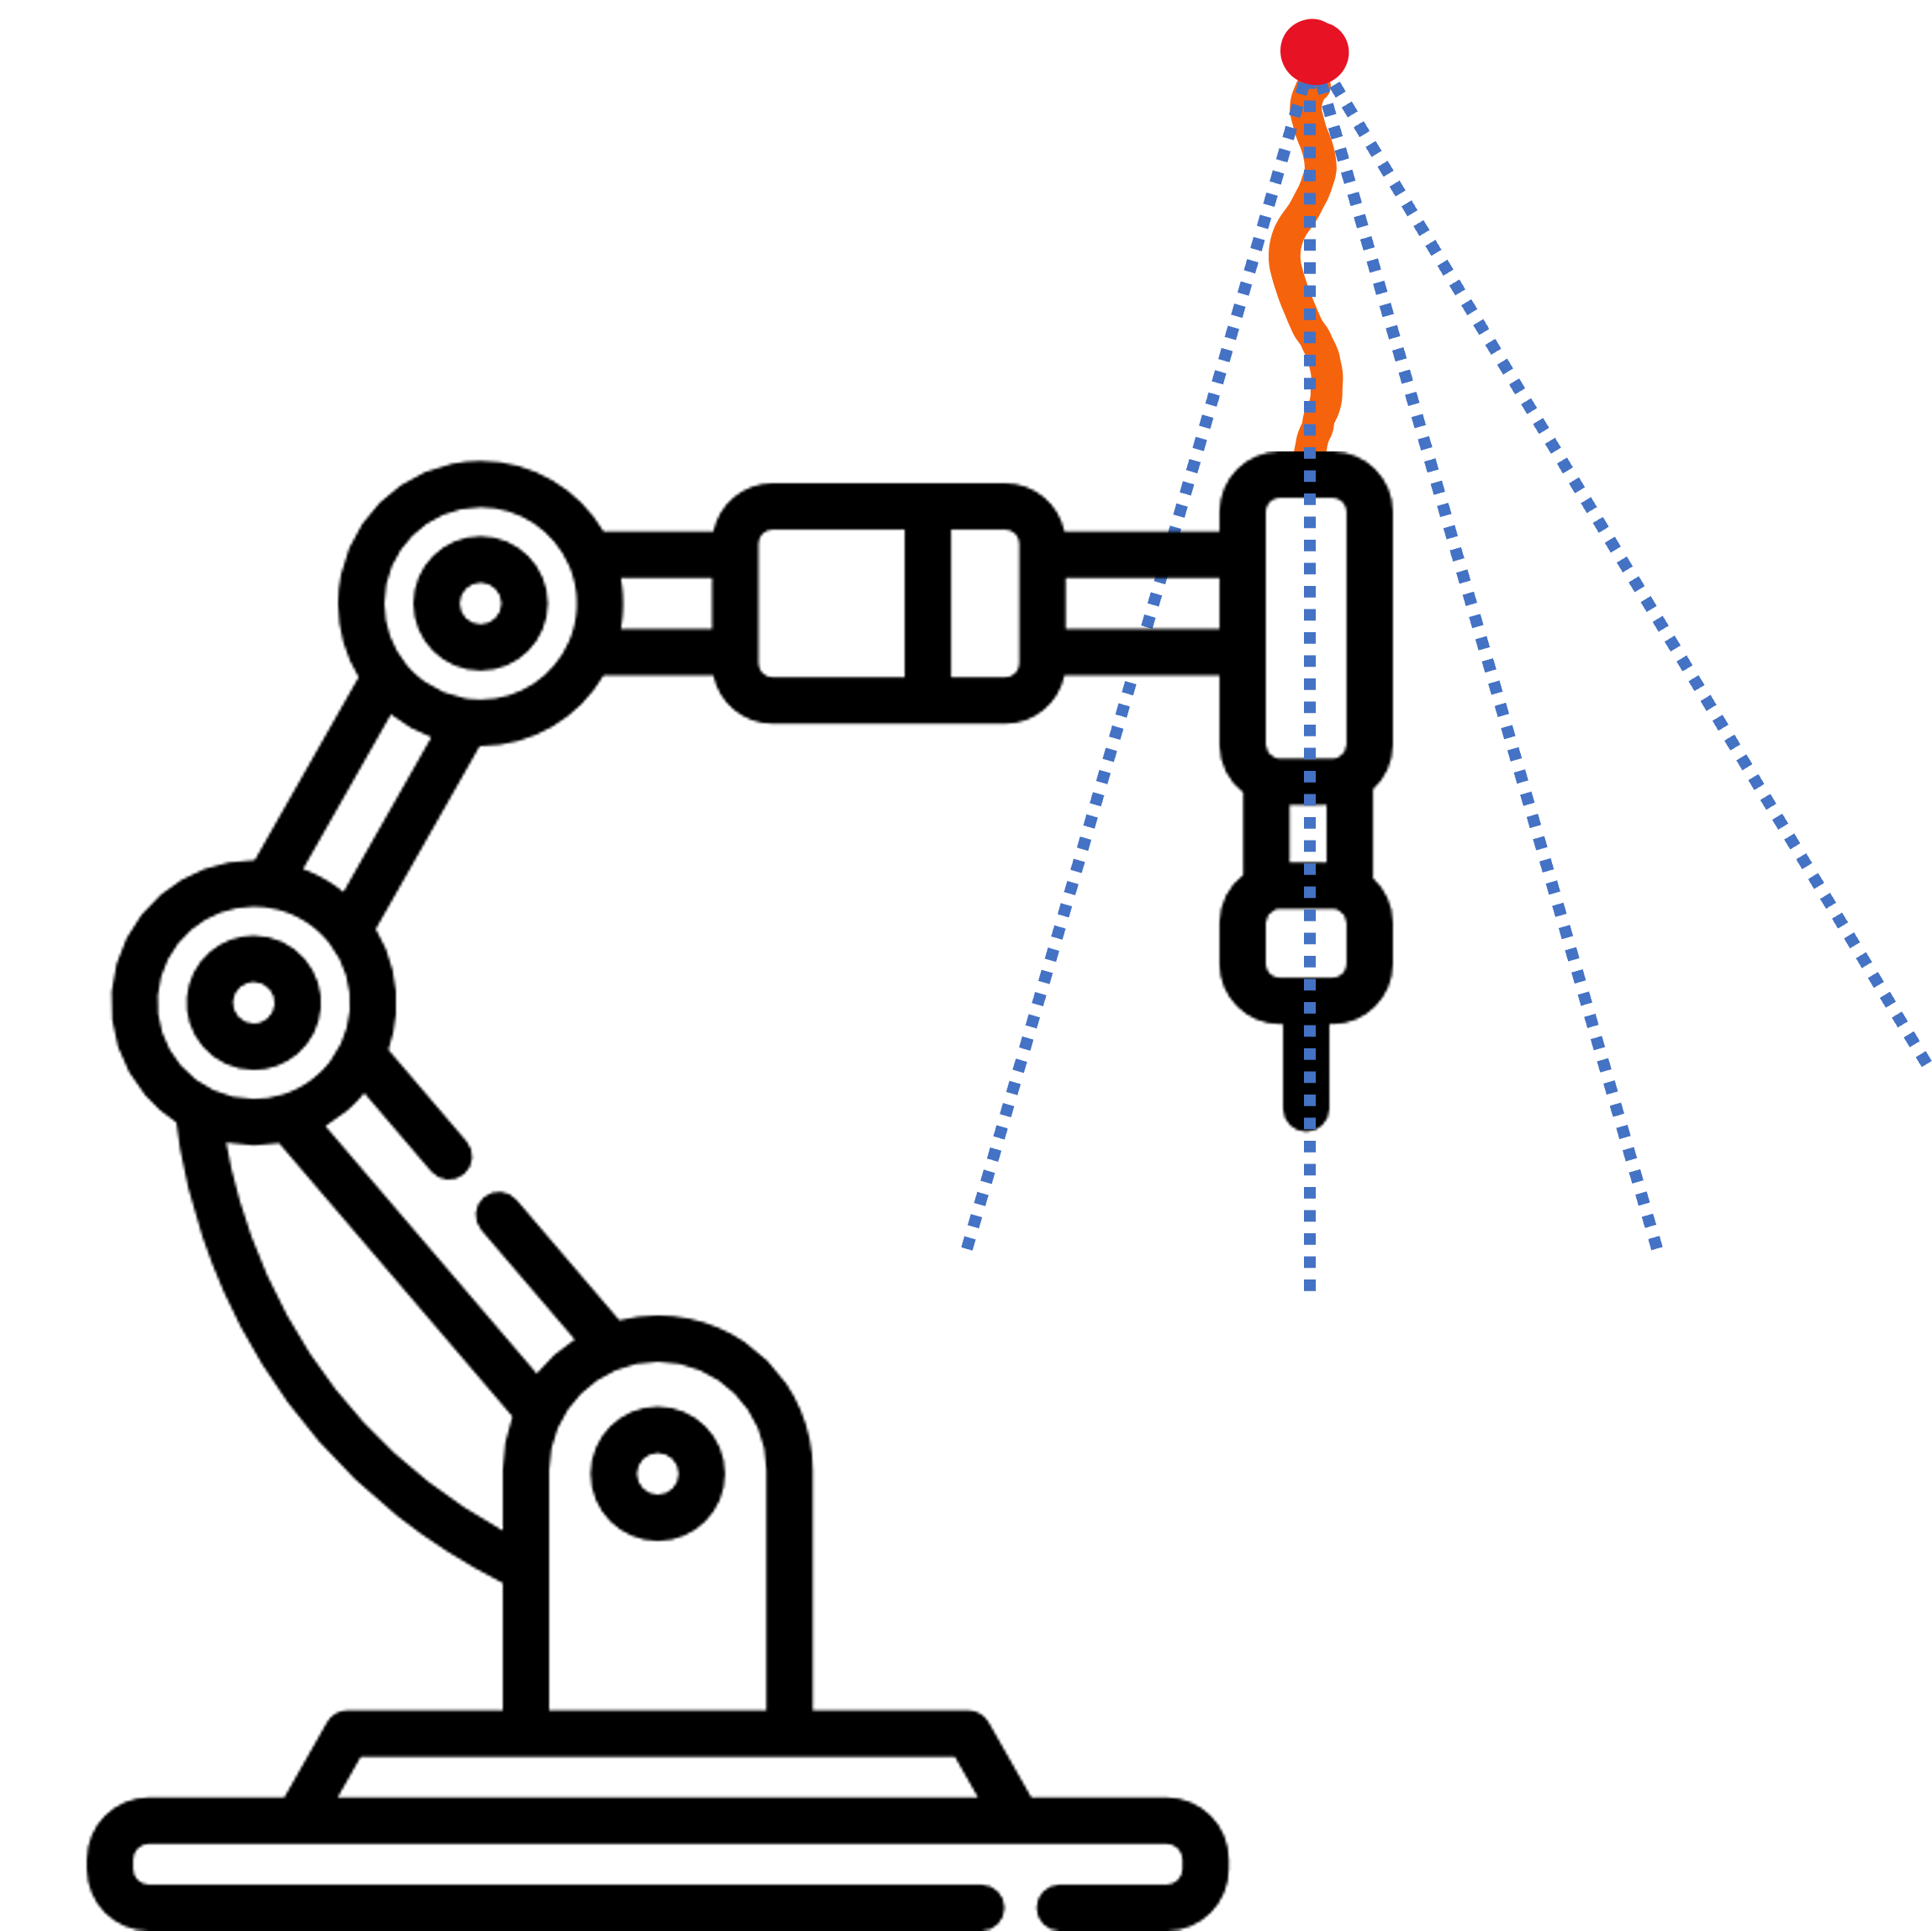
\includegraphics[width=.35\textwidth]{figures/angle.png}}}%
	\caption{Two examples for optimal orientation along a vector in 2D}%
	\label{OOPti}%
\end{figure}



To minimize the deviation from the optimal vector or vanishing point, the redundant degrees of freedom can be utilized. One approach is to analyze the deviation and track it over time, creating a time series. Each element in this time series can be squared or cubed, depending on the weight assigned to small and constant deviations versus large but short offsets. The time series is then summed up to form a scalar value, which can be used to calculate the local score through the variation method.


Figure \ref{deviation} illustrates an example of how the scalar value is calculated. It is evident that when cubing the time series, more importance is placed on the larger deviations rather than small deviations.


\begin{figure}[H]
	\centerline{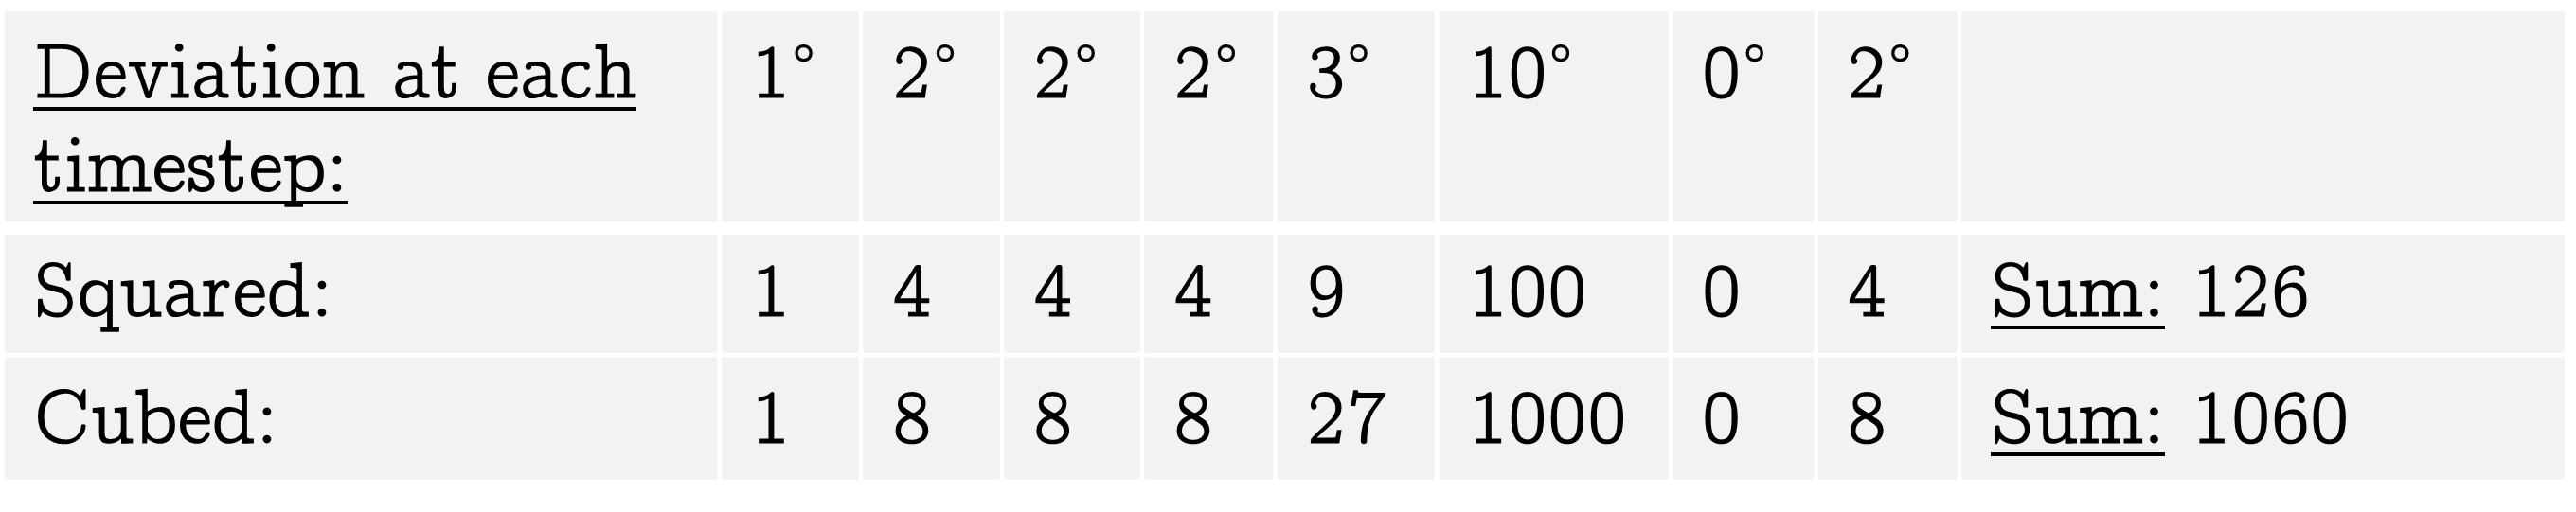
\includegraphics[width=.9\textwidth]{figures/devi.png}}
	\caption{From time-series of the deviation vector to scalar value}
	\label{deviation}
\end{figure}
 

\subsection{Singularities}

In Chapter \ref{Singularity avoidance}, the concept of singularities in robotic manipulators is discussed. Singularities occur when the robot's joints align in a way that limits its motion by reducing one or more degrees of freedom. To avoid singularities, it is important to optimize the boundary conditions in the redundant degrees of freedom. The singularity analysis, as described in Table \ref{procesparameters}, can be represented either as a scalar value or as a time series that classifies each position based on its proximity to a singularity.

The scalar value can represent the overall smallest eigenvalue of every Jacobi matrix. For this, every pose needs to be analyzed. After calculating the Jacobi matrix, all eigenvalues encountered are examined, and only the smallest one is recorded and used to calculate the local score. This approach allows for an analysis of the overall toolpath rather than specific poses.

Alternatively, a time series can be used where the determinant, not the eigenvalues, is recorded and stored. By analyzing this time series, it becomes possible to directly associate the robot's movements with its proximity to a singularity. This enables a more precise understanding of where the robot's motions are close to a singularity, allowing for subsequent optimizations. To transform the time series into a scalar value, the same threshold method described in Chapter \ref{VAJJ} can be applied.
  
  

\subsection{Torch Orientation in WAAM}
The torch orientation parameter in Wire Arc Additive Manufacturing (WAAM), similar to the cable routing orientation parameter, analyzes the angle at which the welding torch is positioned during the process. This parameter is specific to WAAM and ensures that the torch is at the optimal angle for welding. Achieving material deposition in the direction of gravity is crucial for obtaining the best results. The orientation of the Tool Center Point (TCP), which represents the welding torch tip, can be determined either through the forward kinematics approach or by extracting it directly from the G-code.

In both the forward kinematics approach and the G-code, the rotation is described as the rotation around the A, B, and C axes. However, the necessary information for torch orientation is simply the angle between the tilted Z-axis of the tool and the vector of gravity. To obtain this information, a dot product is performed between the rotation matrix and the Z-axis of the base coordinate system. This yields a vector corresponding to the tilted Z-axis of the tool. The enclosed angle can then be calculated using the scalar product. This step assumes that the defined coordinate system is oriented in a way that aligns the Z-axis parallel to the gravity vector.

Figure \ref{tilt} gives a visual example in 2D on how the Z-axis of the tool is deviating from the vector of gravity.

\begin{figure}[H]
	\centerline{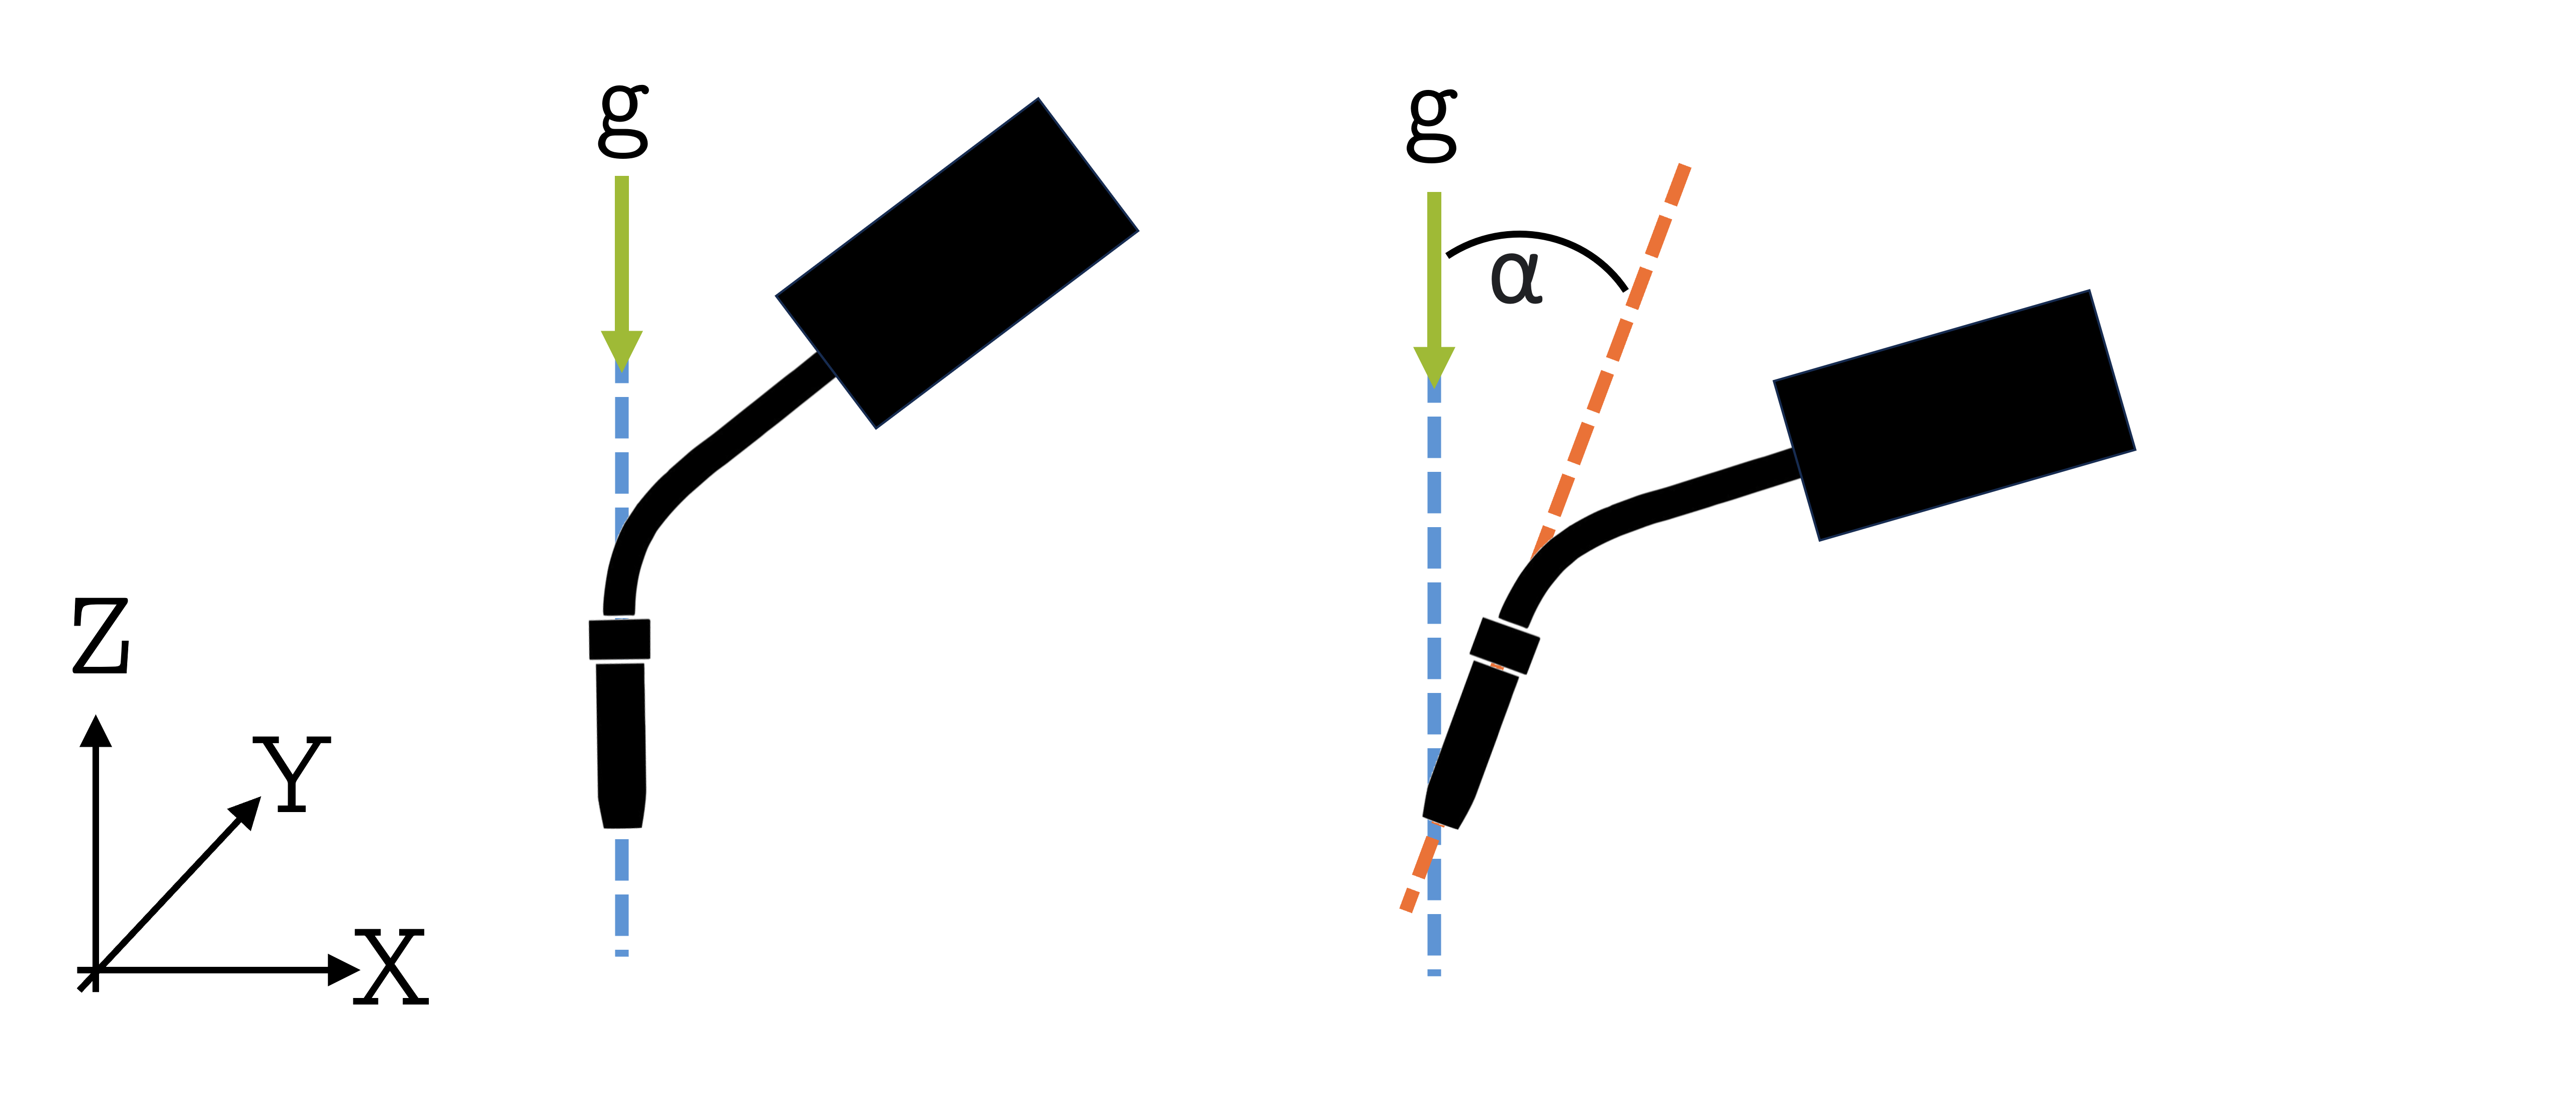
\includegraphics[width=.5\textwidth]{figures/ttilt.png}}
	\caption{Example of non-optimal tilt in the welding torch}
	\label{tilt}
\end{figure}

To quantify the torch orientation parameter, it is recorded in a time series format. To obtain a scalar value for this parameter, all the values can be squared, cubed, or subjected to other mathematical operations, and then summed up. This process is similar to the one described in Chapter \ref{RO} for the cable routing orientation parameter.



\section{Summery for Boundary Condition Evaluation}
\section{General Methodology for Process Optimization}
\subsection{Without NX}
\subsection{With NX}%% ADD ME !!!!!!!!!!!!!!!!!!!!
%% !TeX spellcheck = en_US
\chapter{Implementation and Validation}%

The first step in the validation process involves selecting a manufacturing machine and constructing a fundamental model that captures the kinematics and dynamics. In this case, a simple articulated robot is chosen as the manufacturing machine. To test the method in a straightforward scenario, initial tests are conducted on a 6-\acrshort{DoF} model with a 5-\acrshort{DoF} toolpath. The sixth \acrshort{DoF}, which represents rotation around the Z-axis, is freely defined and utilized for optimization purposes. Once this simple model is successfully validated, an additional redundant \acrshort{DoF} is introduced by incorporating the tilt of a rotary-tilt table.

After establishing the basic mathematical model, an optimization algorithm is implemented to determine the optimal values for each redundant \acrshort{DoF} in order to optimize the process variables. This optimization algorithm takes into consideration the specific constraints and objectives of the industrial robot, such as minimizing direction changes or joint accelerations.

%After that, the goal is to incorporate this method with a selected \acrshort{CAM} software to be tested in more complex scenarios.


\section{Simple Implementation}%
\subsection{Modeling a 6-DoF Robot}
To test the proposed method, a simplified articulated industrial robot with 6-\acrshort{DoF} is utilized as a model. A visual representation of this robot can be seen in Figure \ref{robotprog}. The Denavit-Hartenberg (\acrshort{DH}) parameters for this robot are provided in Table \ref{DHp}. These parameters are crucial for describing the geometry and kinematics of the robotic arm. They establish the relationship between adjacent links in the kinematic chain of the robot.

The \acrshort{DH} parameters consist of various values, including link lengths, link twists, and link offsets. In this particular model, \textit{a} represents the link lengths between adjacent joints, \textit{alpha} represents the link twists or rotations around the Z-axis between adjacent joints, and \textit{d} represents the link offsets or distances along the Z-axis between adjacent joints. The units of \textit{a} and \textit{d} are set in millimeters, while the rotation \textit{alpha} is defined in degrees.

It is worth noting that the last rotation is defined in the negative direction. This convention is employed to ensure that the end of the final joint can be interpreted as the tip of a tool without requiring additional transformations from the flange to the \acrshort{TCP}.

\begin{table}[H]
	\centering
	\begin{tabular}{||l|l||}
		Parameters  & Values \\
		\hline
		\hline
		\hline
		a in [mm] 	&		[200, 900, 150, 0,   150, 0] \\
		alpha in [°]	&  	[90,  0,   90,  -90, 90,  -90] \\
		d in [mm]	& 		[600  0,   0,   800, 0,   200]\\
		
		\hline
		\hline
	\end{tabular}
	
	\caption{DH-parameters for the modeled robot}
	\label{DHp}
\end{table}

The schematic of the modeled robot can be observed in Figure \ref{schema}. In this specific configuration, all joints are in their initial positions with no rotation applied.\newline

\begin{figure}[H]
	\centerline{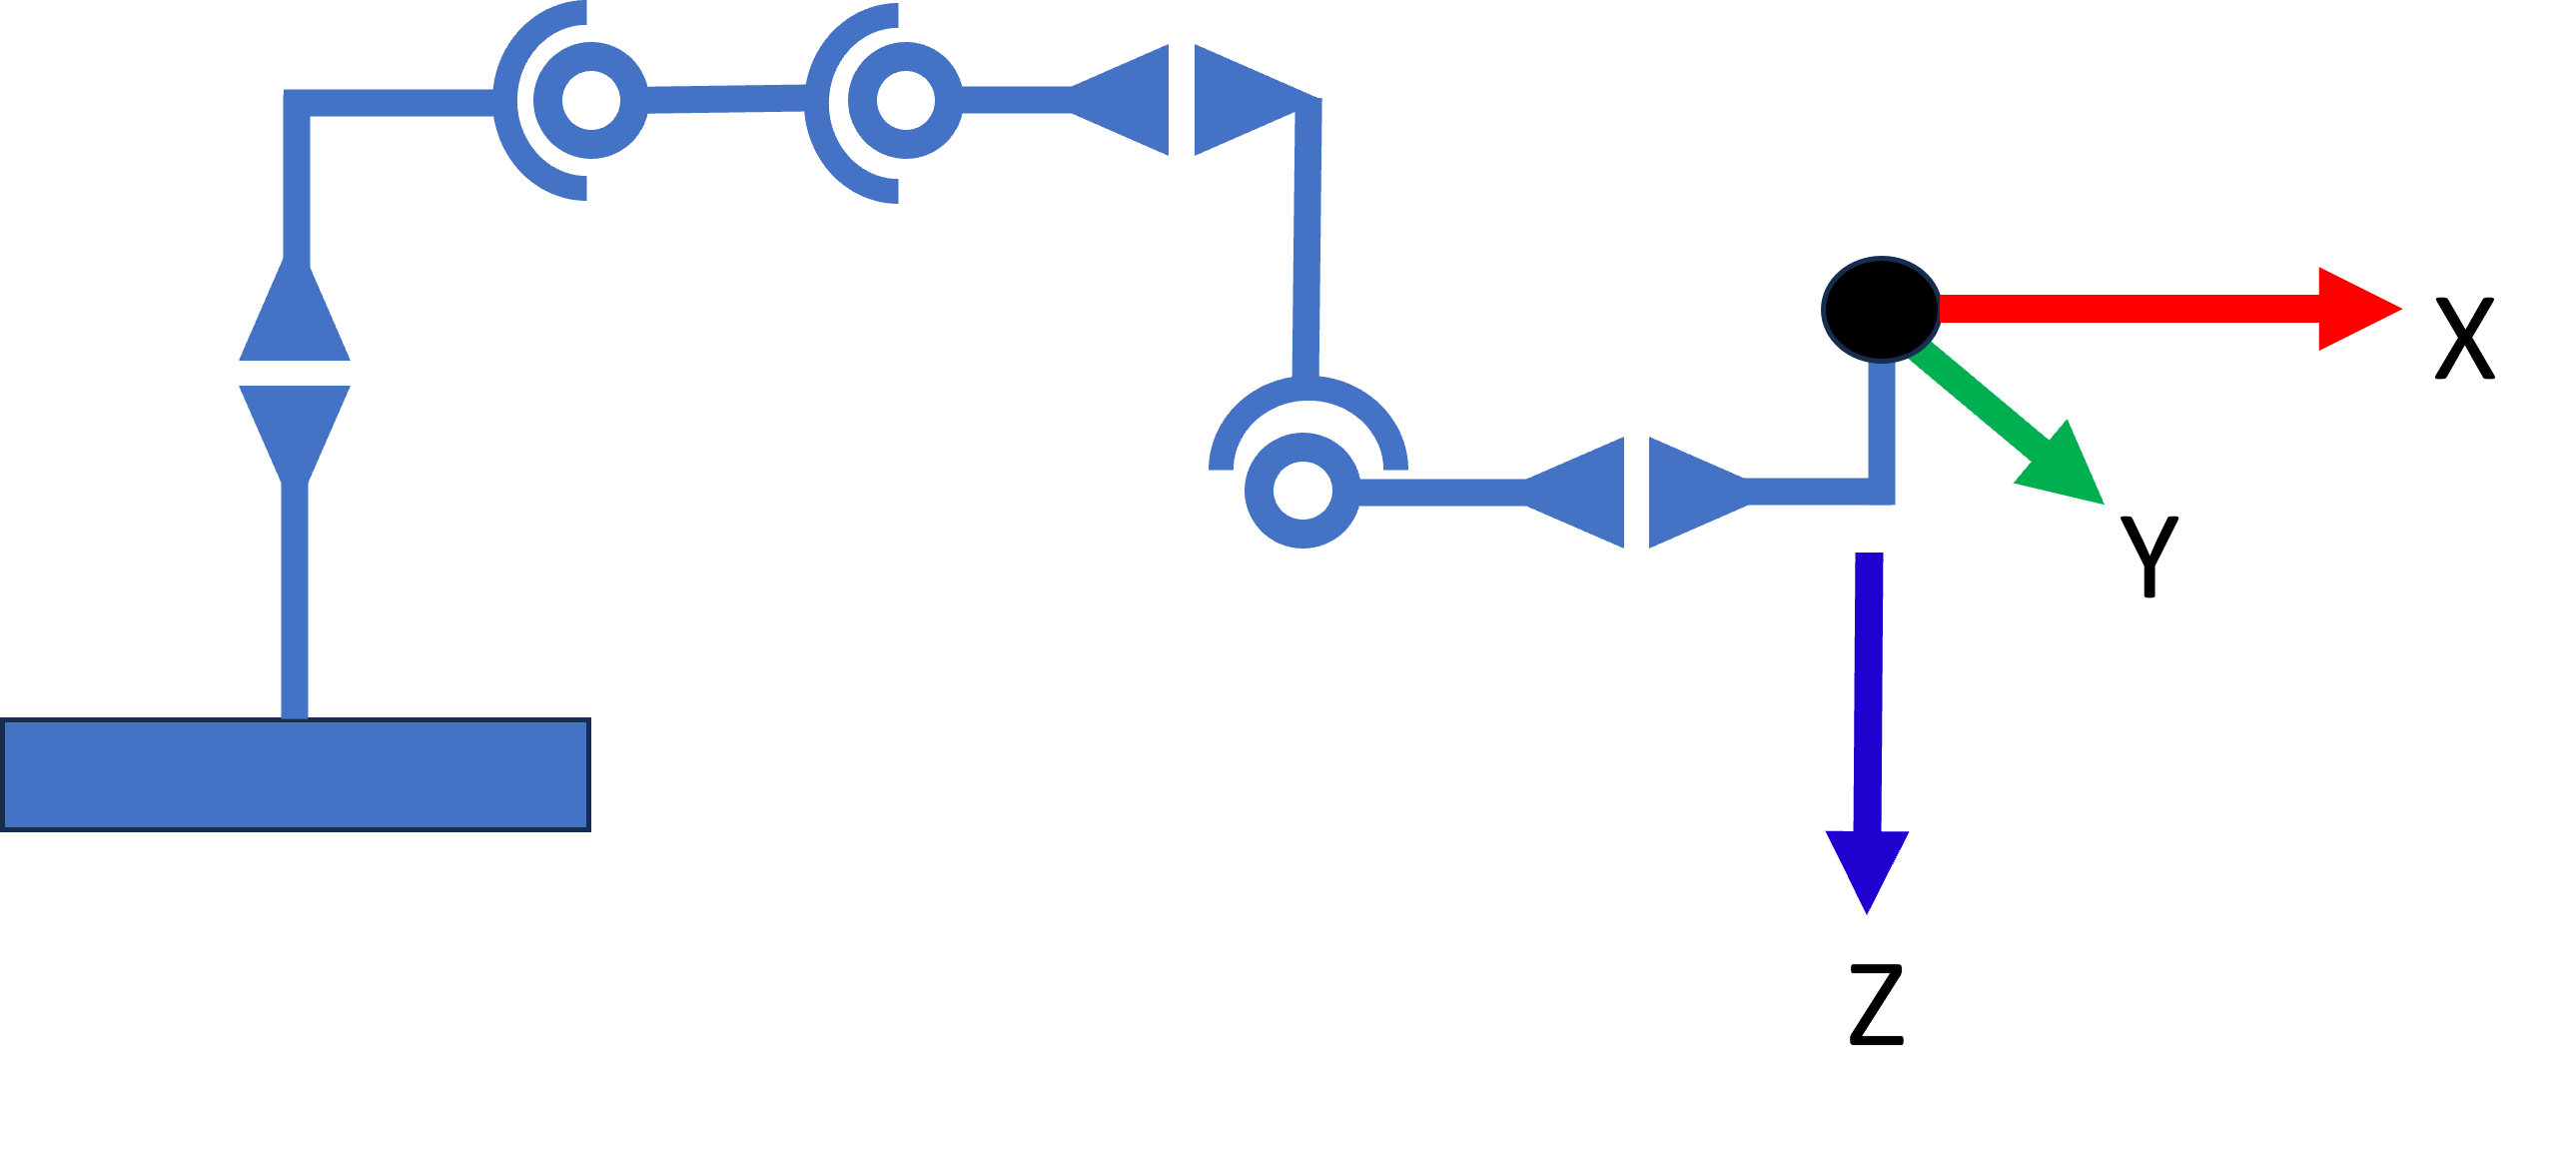
\includegraphics[width=0.7\textwidth]{figures/schema.png}}
	\caption{Schematics of the modeled robot}
	\label{schema}
\end{figure}

Figure \ref{robotprog} depicts the robot modeled using Python in combination with the \textit{Matplotlib} library. The joint positions, in degrees, are as follows: [2, 75, -45, -88, -91, 61], corresponding to joints 1 to 6, respectively. The colored arrows shown in the figure represent the coordinate axes of the \acrshort{TCP}. For simplicity, the \acrshort{TCP} is considered to be the endpoint of the last joint. The X-axis of the \acrshort{TCP} coordinate system is represented in red, while the Y-axis and Z-axis are denoted by the colors green and blue, respectively. The first link of the robot, originating from the point X=0, Y=0, Z=0 in the world coordinate system, is displayed in green. The individual joints are represented by red dots.

\newpage

 \begin{figure}[H]
	\centerline{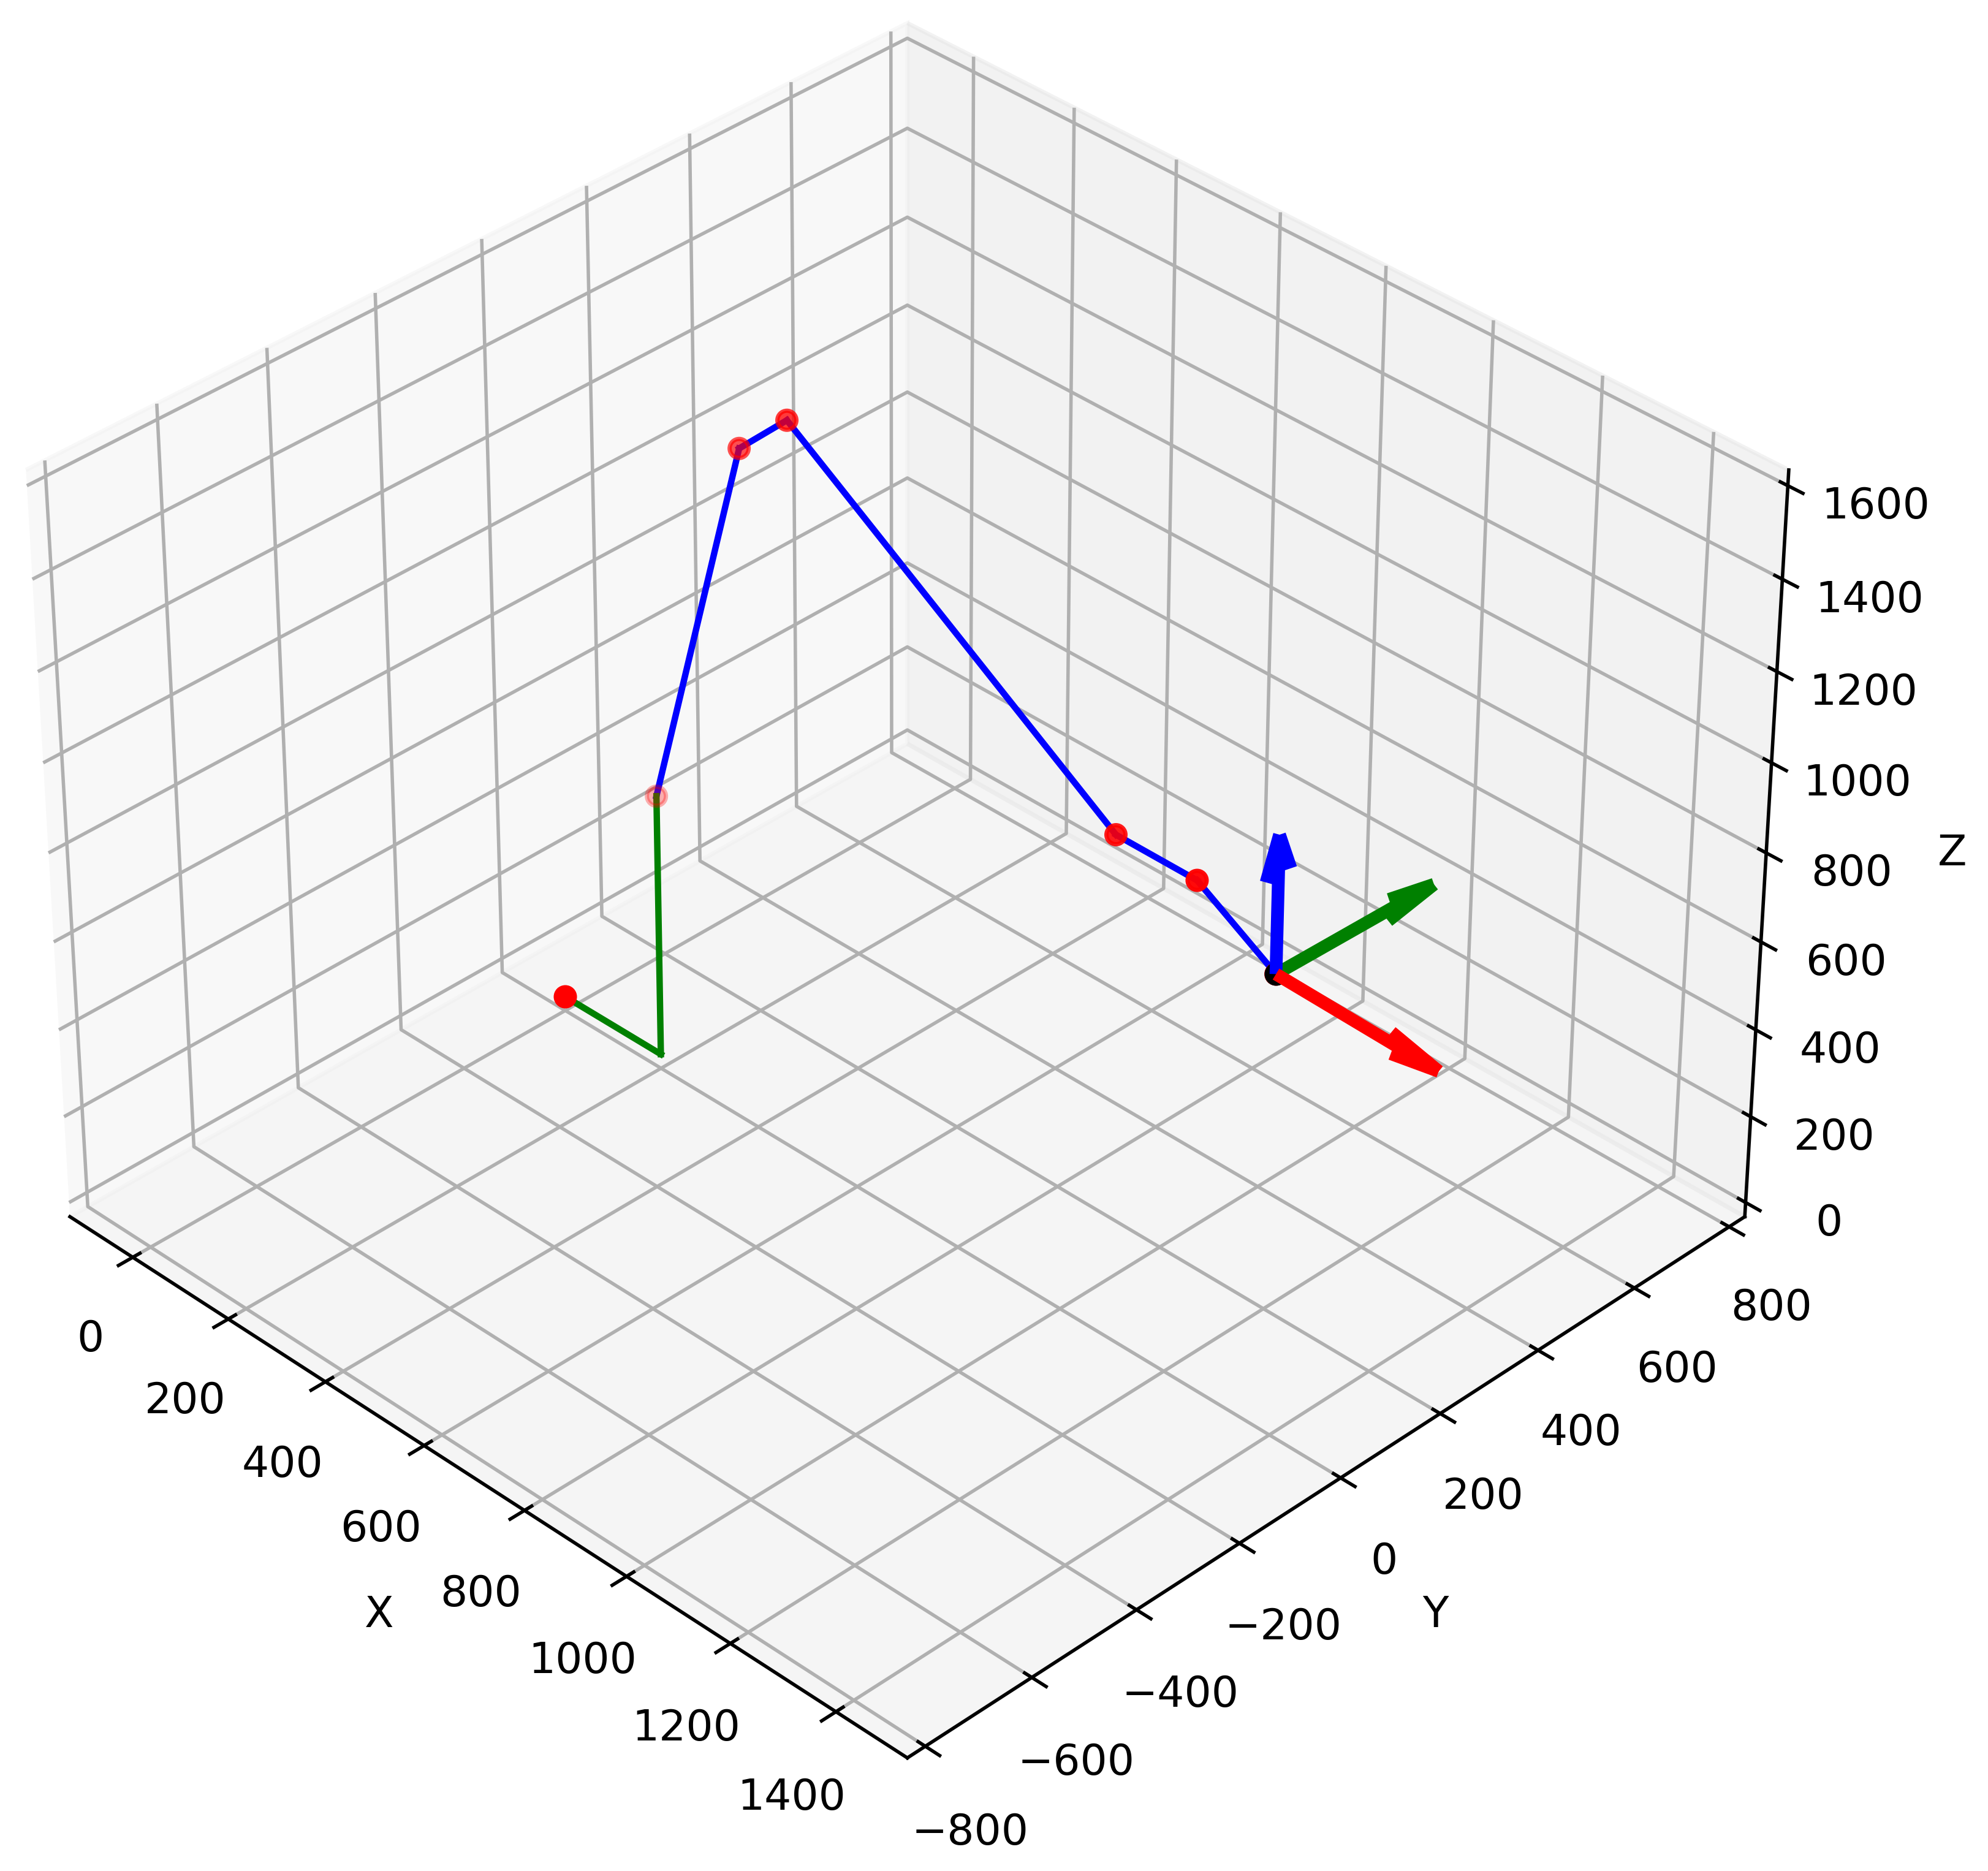
\includegraphics[width=0.9\textwidth]{figures/robotprog.png}}
	\caption{Visualization of the modeled robot in Python}
	\label{robotprog}
\end{figure}


\subsection{Modeling a Basic Toolpath}\label{MBT}
Before analyzing the process variables, it is necessary to define a toolpath for the \acrshort{TCP} to follow. For that case, three options are presented, each consisting of 3000 coordinates. It should be noted that the redundant \acrshort{DoF} in these cases is the rotation around the Z-axis. This rotation will be adjusted to determine the optimal value for the desired outcome. A and B are held at 0°.

The first toolpath, depicted in Figure \ref{path1}, represents a converging-diverging spiral. Figure \ref{path2} illustrates a converging infinity-loop, and Figure \ref{path3} displays a forward-moving sinusoidal curve. The corresponding equations for these toolpaths are given by Equation \ref{eq1}, Equation \ref{eq2}, and Equation \ref{eq3}, respectively. The variable \textit{iter} ranges from 0 to 3000 and is used to calculate the X, Y, and Z coordinates. Trigonometric functions are utilized with the help of the \textit{Numpy} library. Currently, no rotation (A, B, or C) has been defined. Only the coordinates are specified. Each toolpath has specific dimensions and characteristics. Toolpaths 1 and 2 are continuous, while toolpath 3 exhibits abrupt changes in direction. Only toolpath 1 possesses rotational symmetry.\newpage


\begin{figure}[H]% [H] is so declass\'e!
	\centering
	\begin{minipage}{0.5\textwidth}
		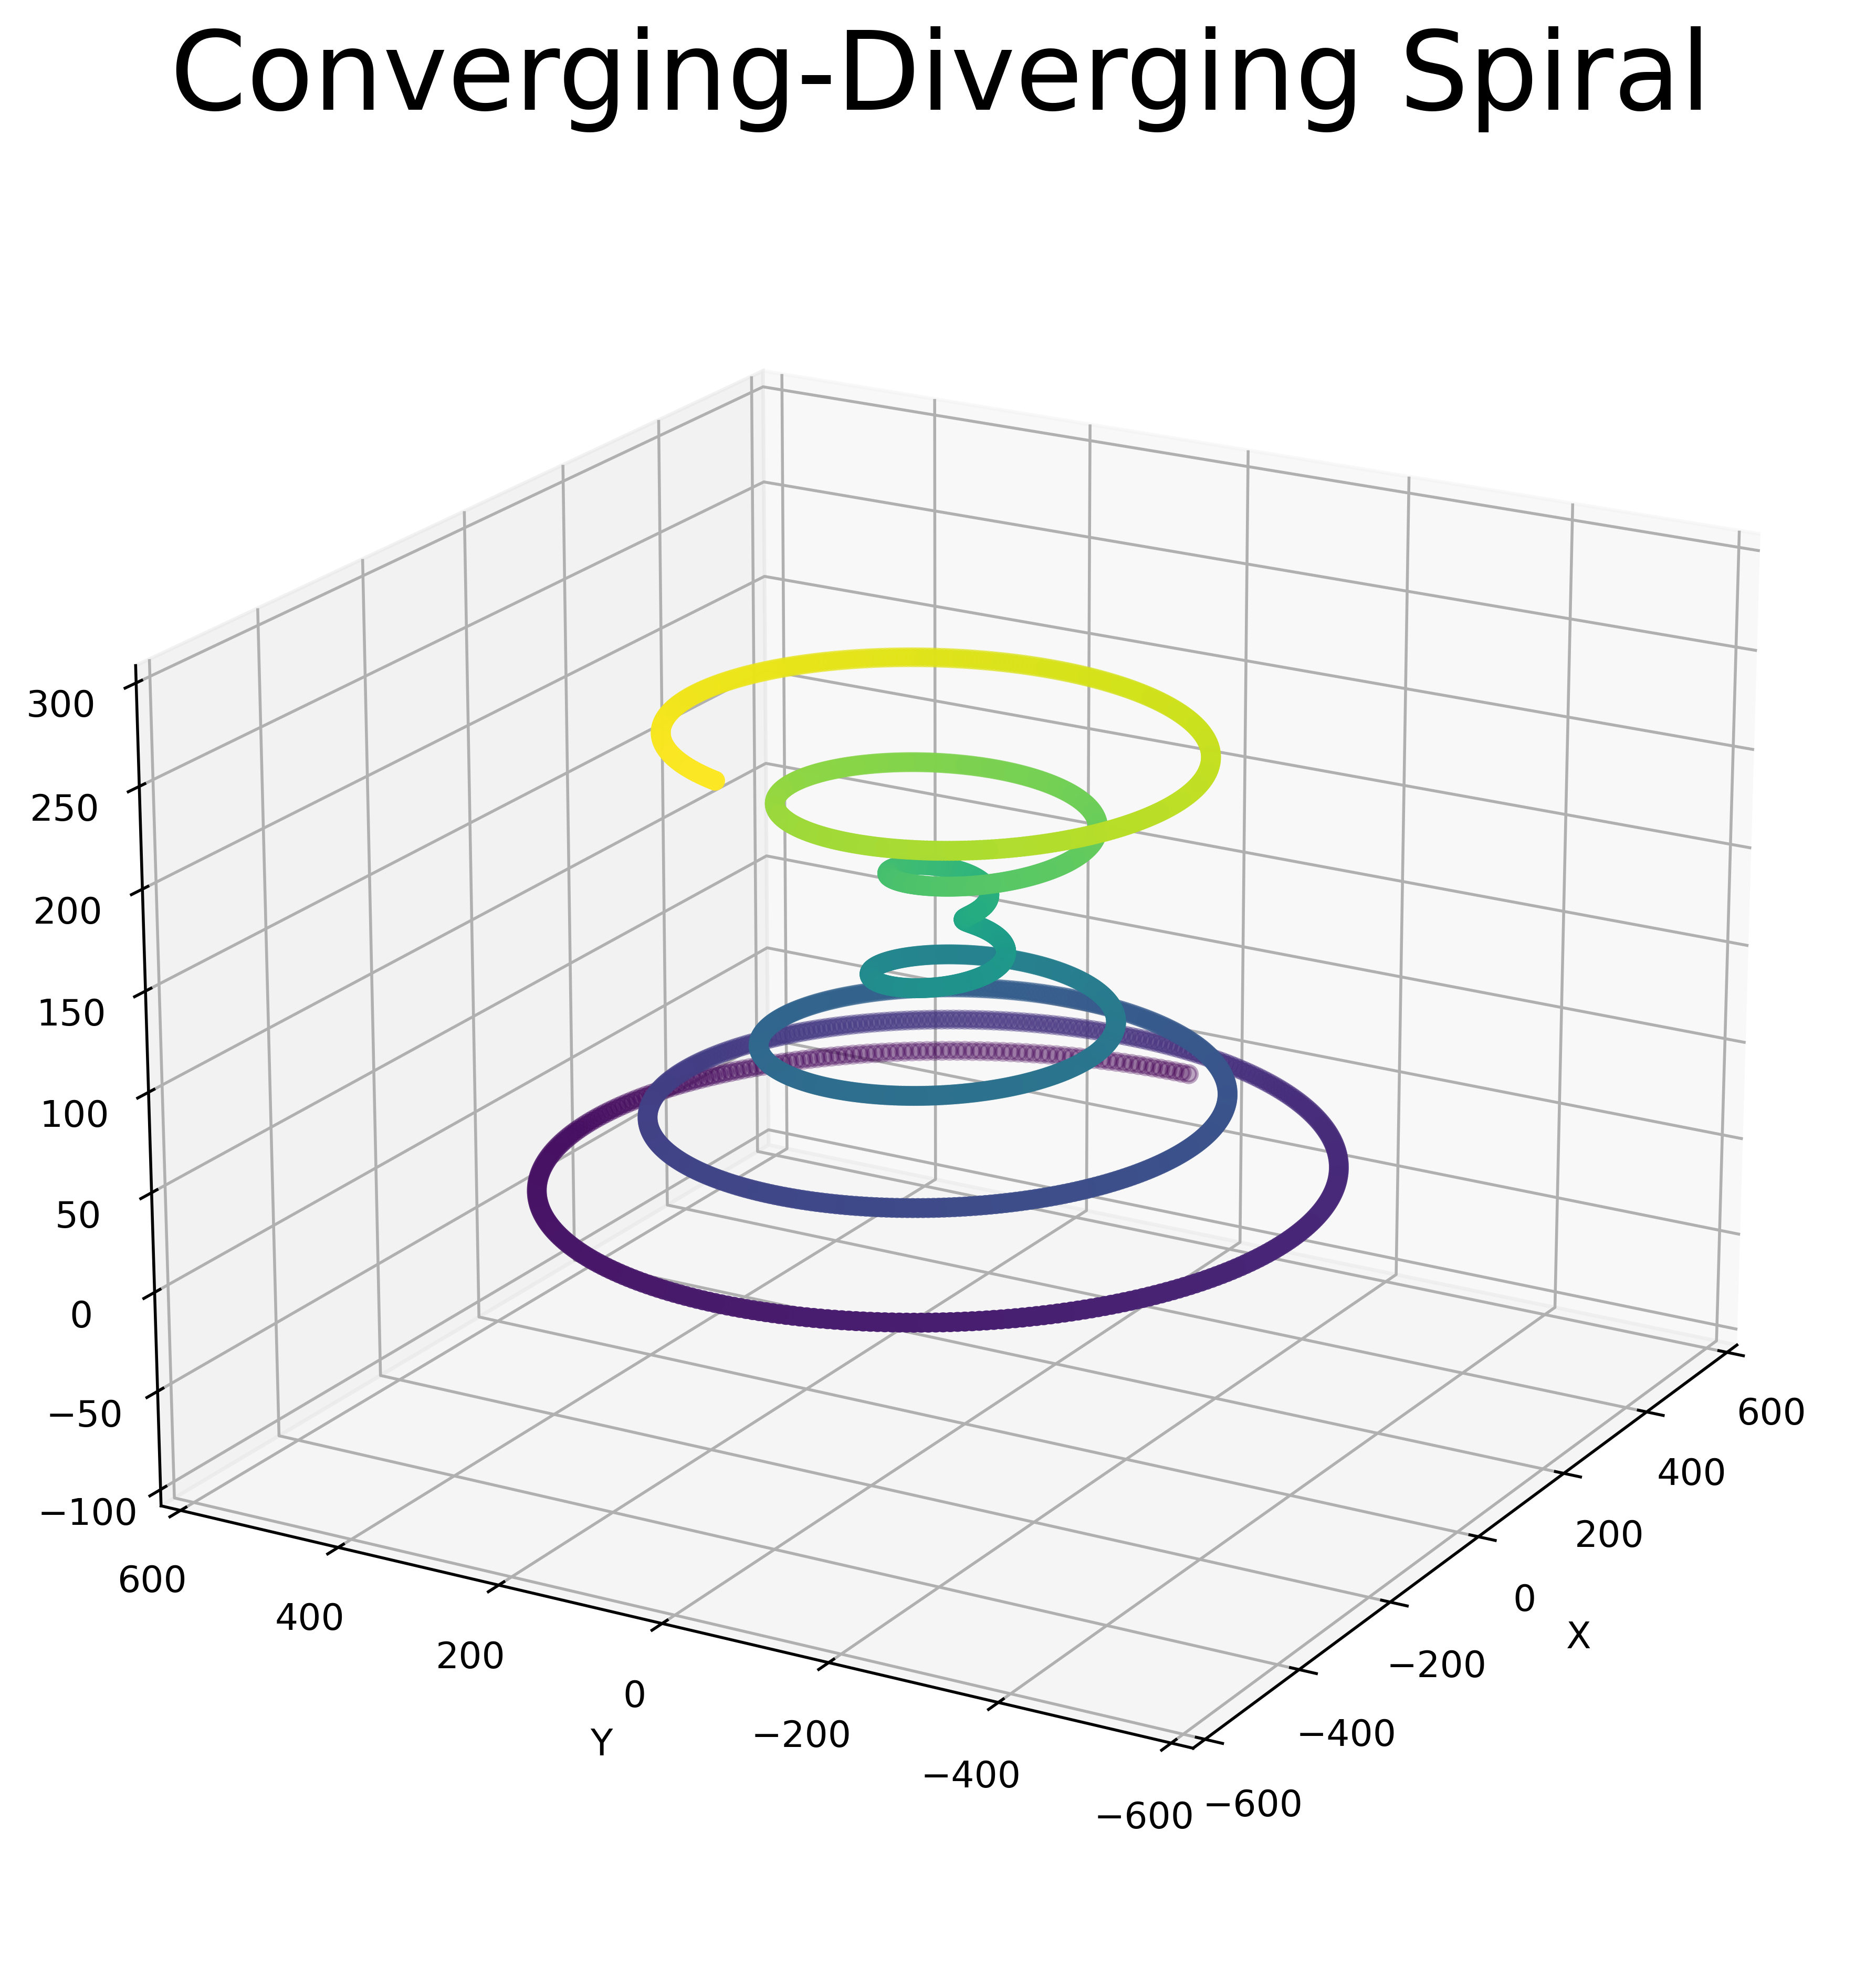
\includegraphics[width=\textwidth]{figures/path1.png}
		\caption{Toolpath 1: Converging-diverging spiral}
		\label{path1}
	\end{minipage}\hfill
	\begin{minipage}{0.5\textwidth}
		\begin{equation}\label{eq1}
			\begin{split}
				x &= cos(iter) * (500 - iter / 3)\\
				y &= sin(iter) * (500 - iter / 3)\\
				z &= iter / 10
			\end{split}
		\end{equation}
	\end{minipage}\par
\end{figure}

\begin{figure}[H]% [H] is so declass\'e!
	\centering
	\begin{minipage}{0.5\textwidth}
			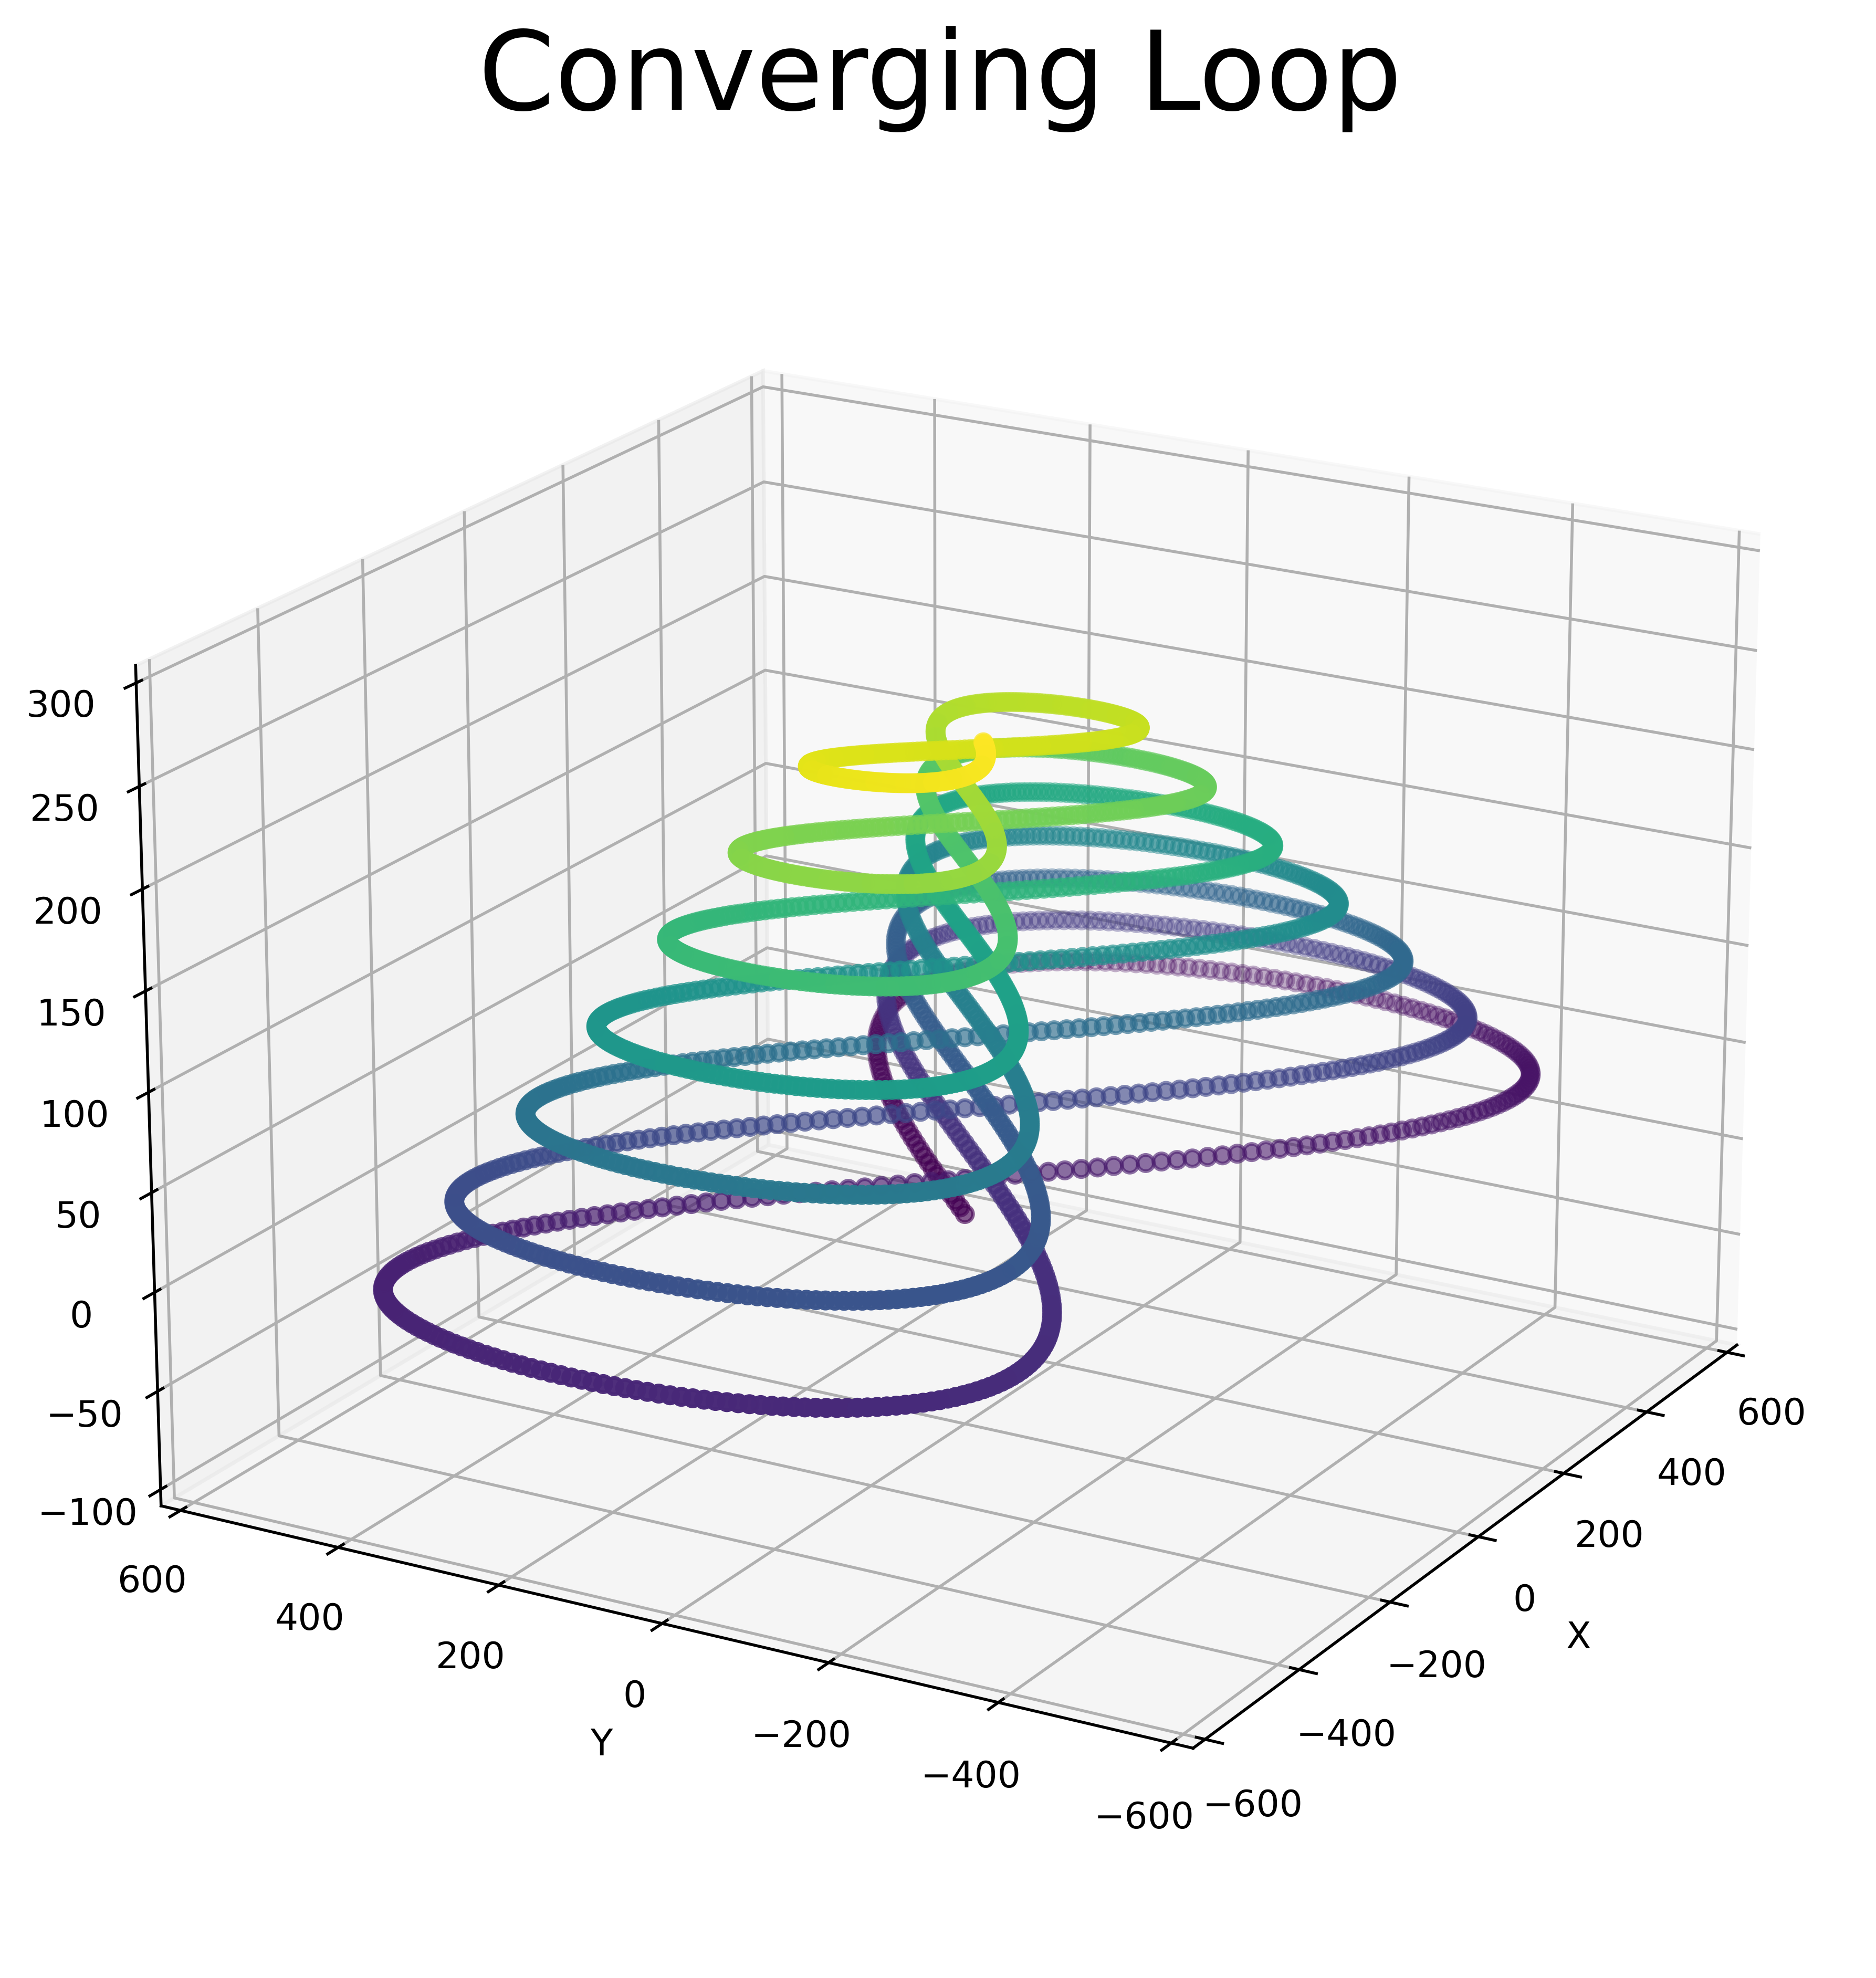
\includegraphics[width=0.95\textwidth]{figures/path2.png}
		\caption{Toolpath 2: Converging infinity loop}
		\label{path2}
	\end{minipage}\hfill
	\begin{minipage}{0.5\textwidth}
		\begin{equation}\label{eq2}
			\begin{split}
				x &= sin(iter) * (400-iter / 5)\\
				y &= sin(iter) * cos(iter) * (500-iter / 6)\\
				z &= iter / 10
			\end{split}
		\end{equation}
	\end{minipage}\par
\end{figure}


\begin{figure}[H]% [H] is so declass\'e!
	\centering
	\begin{minipage}{0.5\textwidth}
		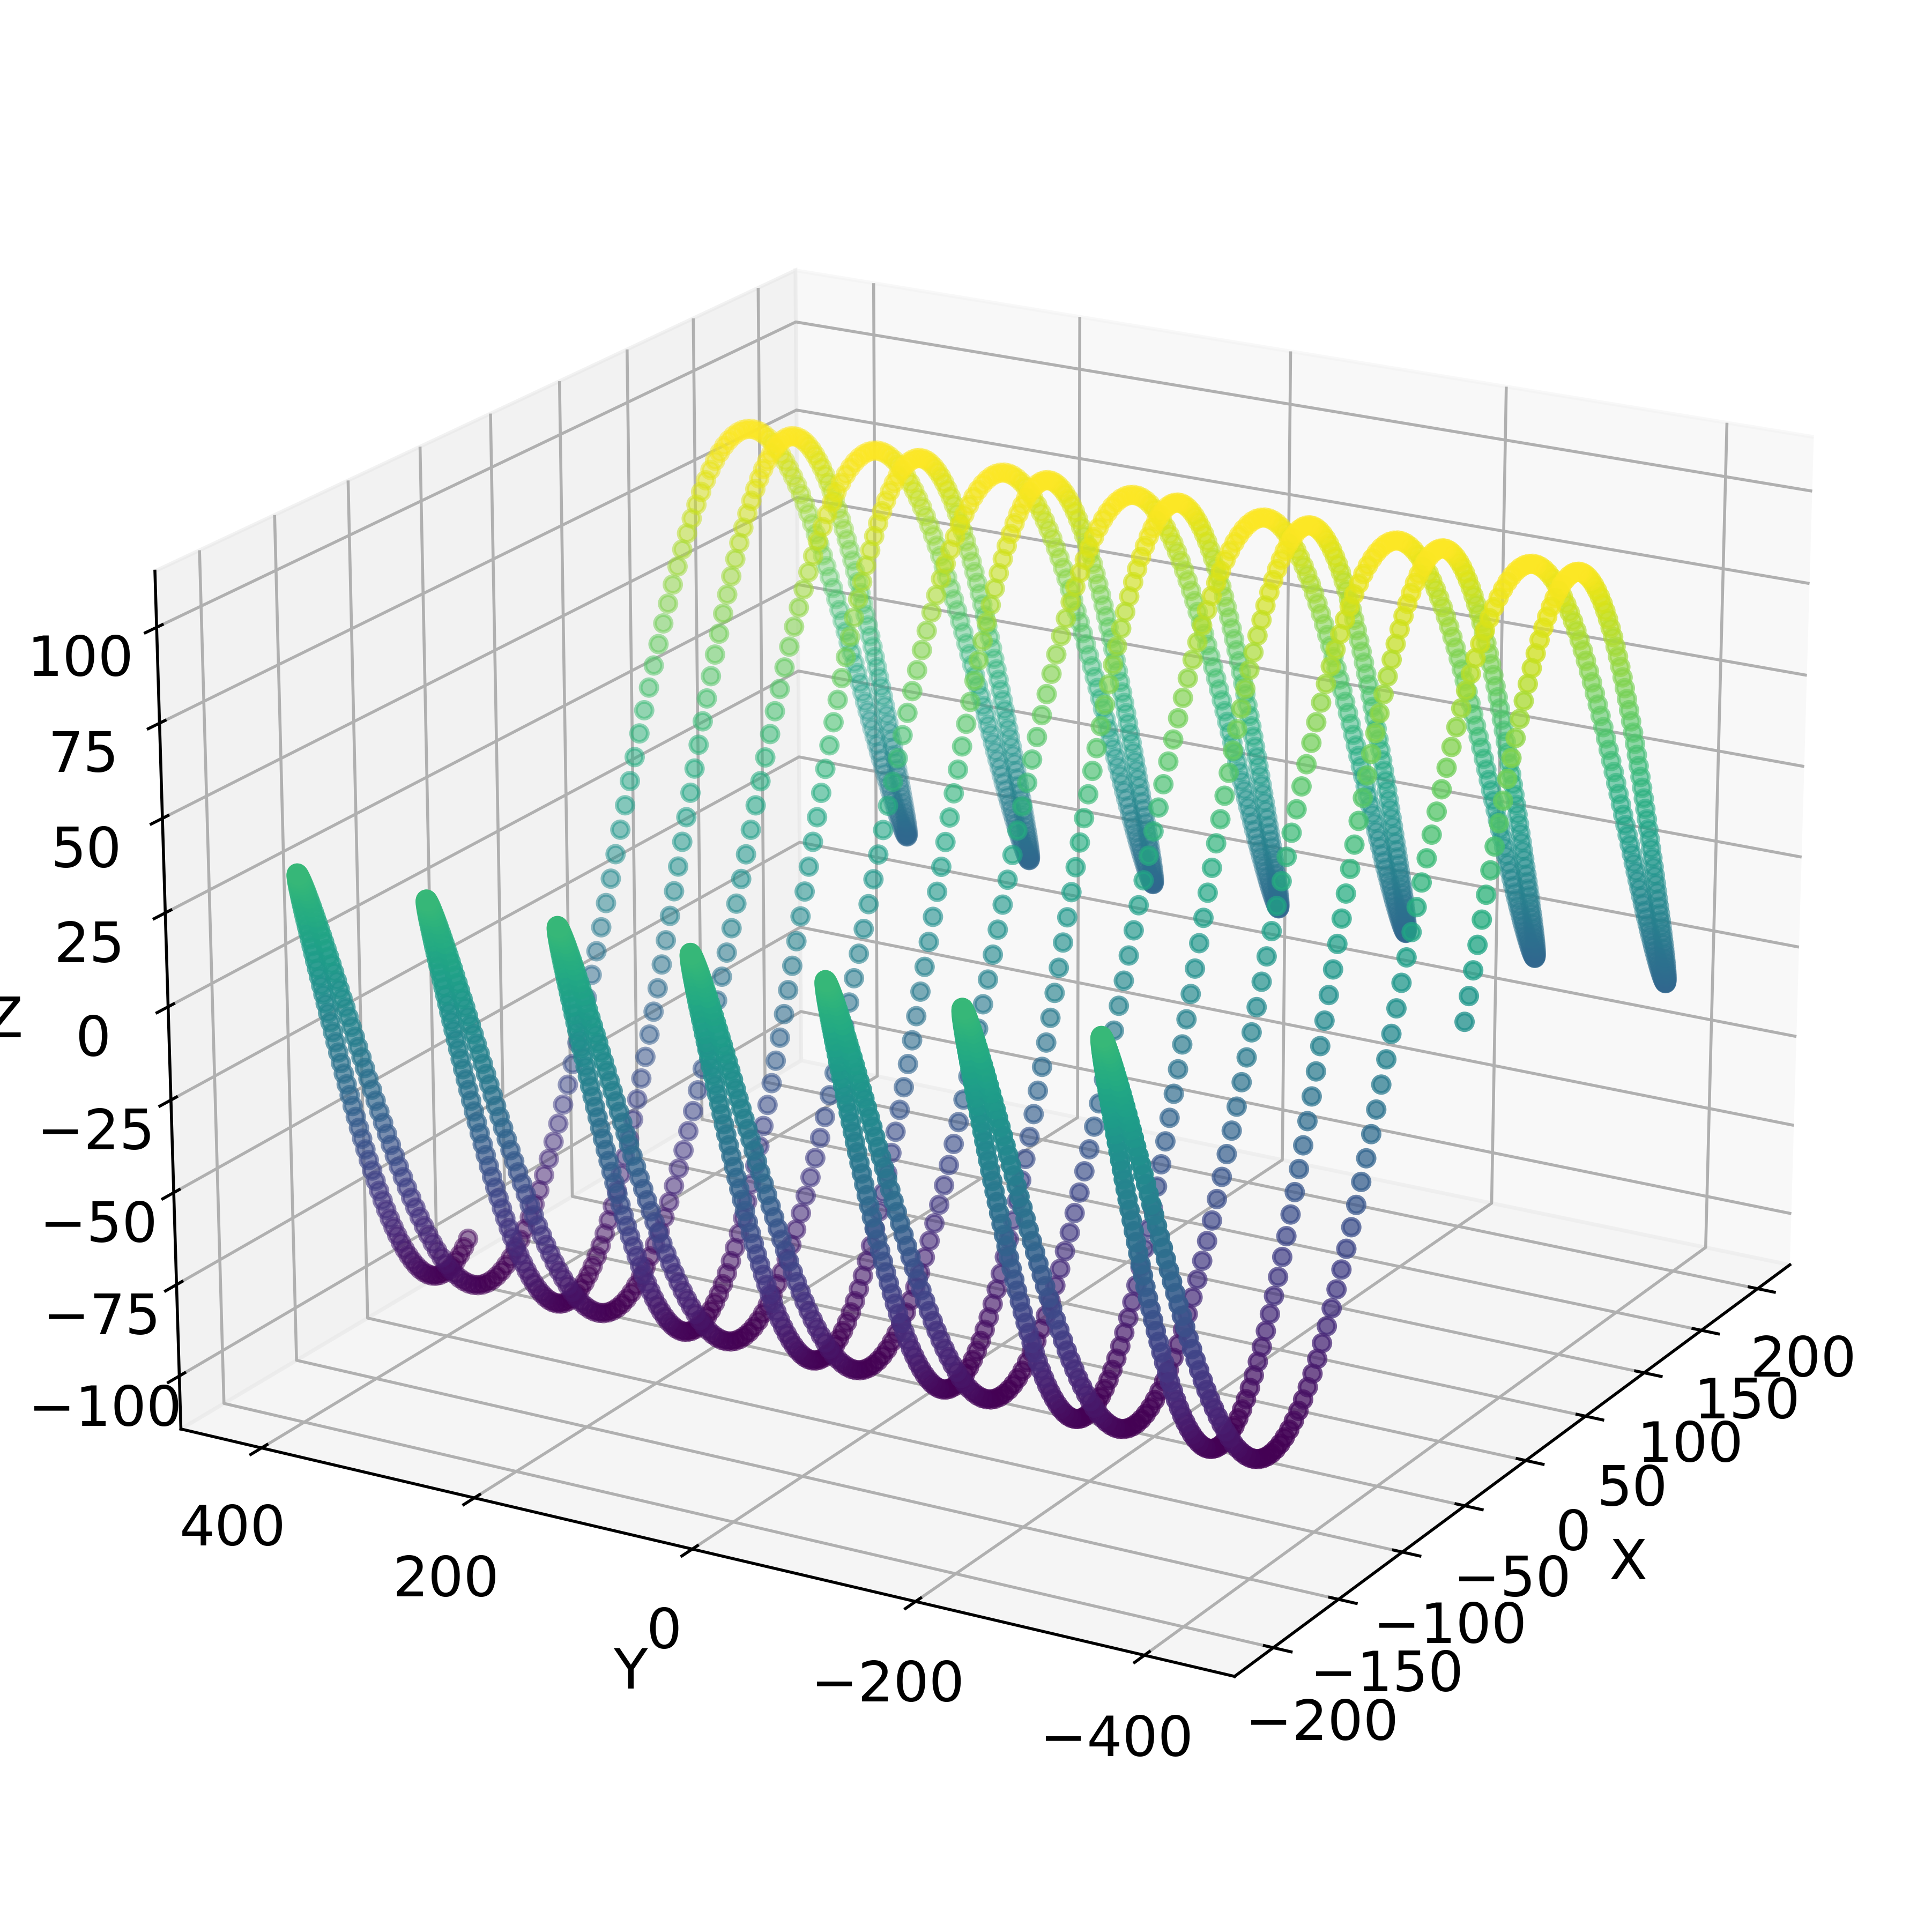
\includegraphics[width=\textwidth]{figures/path3.png}
		\caption{Toolpath 3: Forward moving pendulum oscillation}
		\label{path3}
	\end{minipage}\hfill
	\begin{minipage}{0.5\textwidth}
		\begin{equation}\label{eq3}
			\begin{split}
				x &= sin(iter) * 200\\
				y &= (iter / 3) - (2500/6)\\
				z &= sin(x)*100
			\end{split}
		\end{equation}
	\end{minipage}\par
\end{figure}

\newpage
Figure \ref{TP1robot} illustrates the robot and Toolpath 1 (defined by Equation \ref{eq1}) at the final position of the toolpath. The origin of the toolpath is shifted by X=+1000 and Z=+600 relative to the world coordinate system. No rotations are applied around the X, Y, and Z axes, resulting in A, B, and C being zero. As a result, the coordinate axes of the \acrshort{TCP} are parallel to the axes of the robot's coordinate system (world coordinate system).



\begin{figure}[H]
	\centerline{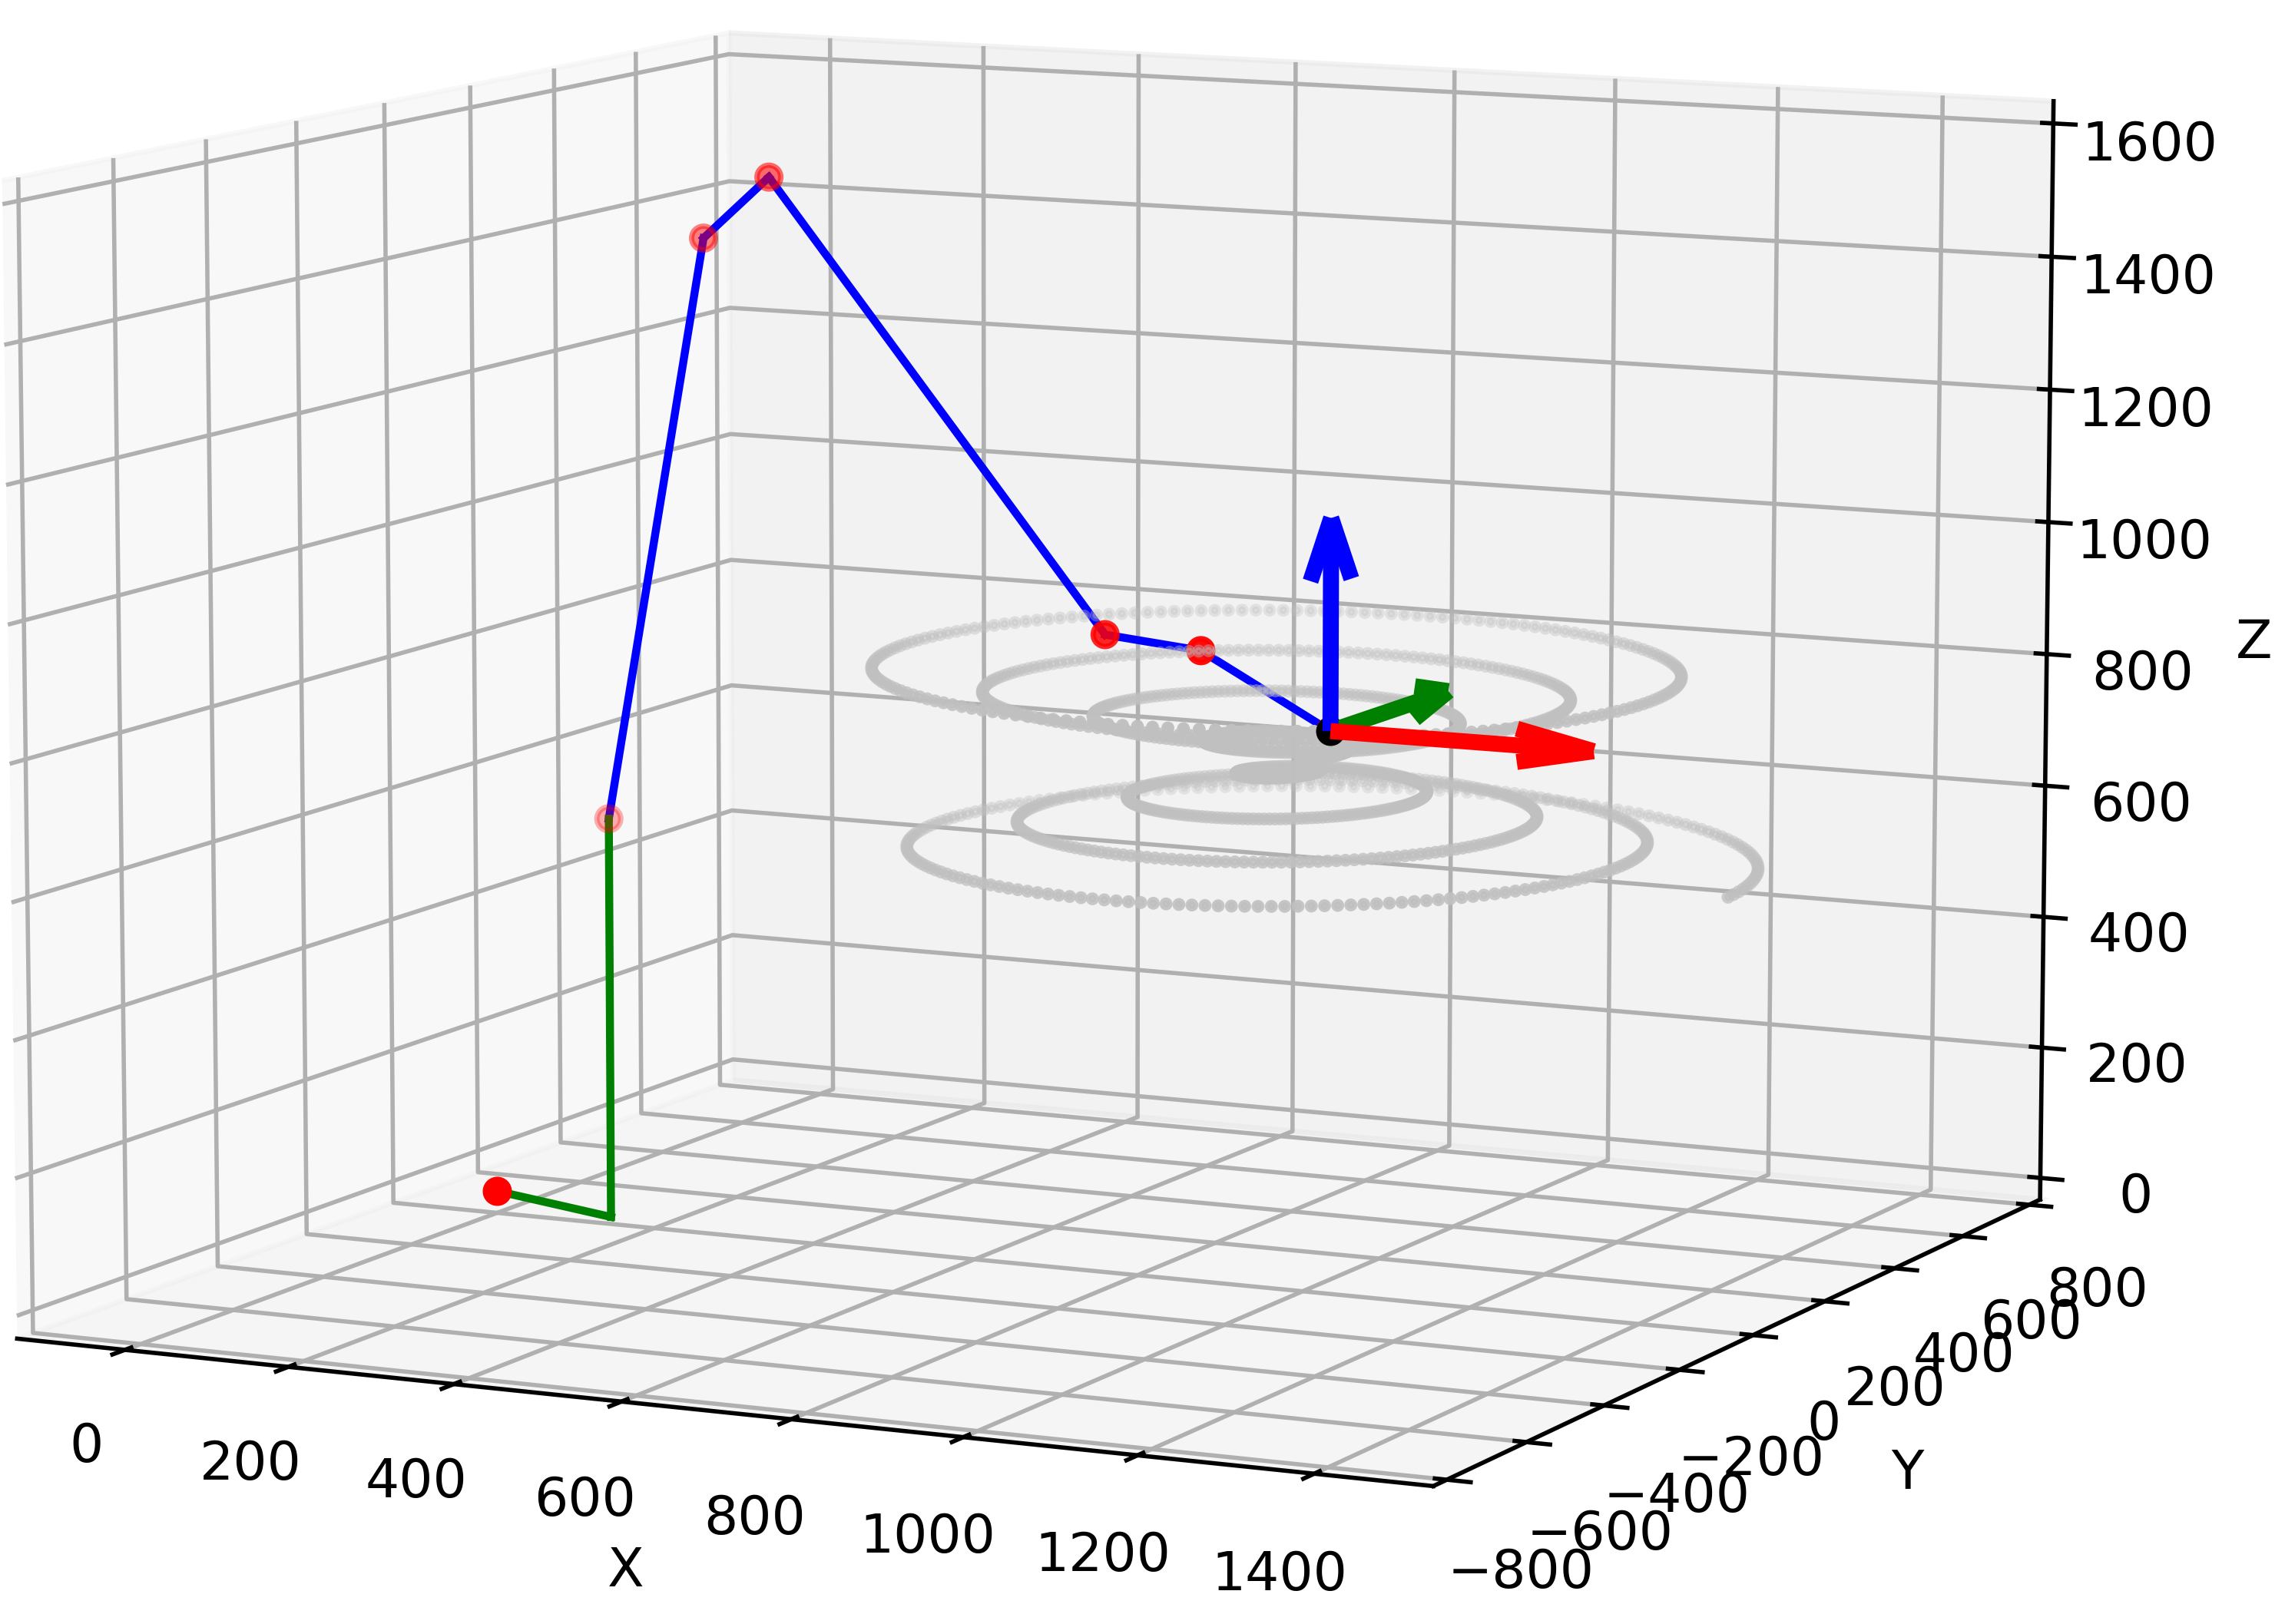
\includegraphics[width=0.9\textwidth]{figures/robotANDpath1.png}}
	\caption{Traversing toolpath 1}
	\label{TP1robot}
\end{figure}




\subsection{Extracting Process Variables}
By utilizing the inverse kinematics algorithm from the Python library \textit{visual\_kinematics}, the joint angles for each coordinate can be computed. To achieve this, the rotations A, B, and C need to be defined. The outcome is a time-series that contains the corresponding joint positions. For all tests, all coordinates must be traversed in equidistant time steps. With this information, it becomes possible to calculate the velocity and other related variables. By transforming all the data from the time-series into scalar values and calculating the local rating, the local and global scores can be determined.
\newpage
\section{Testing and Validation}%

\subsection{Toolpath Evaluation With one Redundant DoF}
%\subsubsection{Obtaining Joint Positions}
As discussed in Chapter \ref{MBT}, the toolpath remains constant with respect to the X-, Y-, and Z-coordinates. The fixed boundary conditions for the robot are that there are no rotations around the X and Y axes, resulting in A and B both being equal to zero. This condition is fixed for the entire toolpath. The user has the ability to set the \acrshort{DoF} for the rotation around the Z-axis, which is the redundant \acrshort{DoF}. Figure \ref{TP1ABC0} displays the variation of each joint over time for toolpath 1. In this specific case, the rotations A, B, and C are all set to 0. The entire toolpath is traversed in 300 seconds.

\begin{figure}[H]
	\centerline{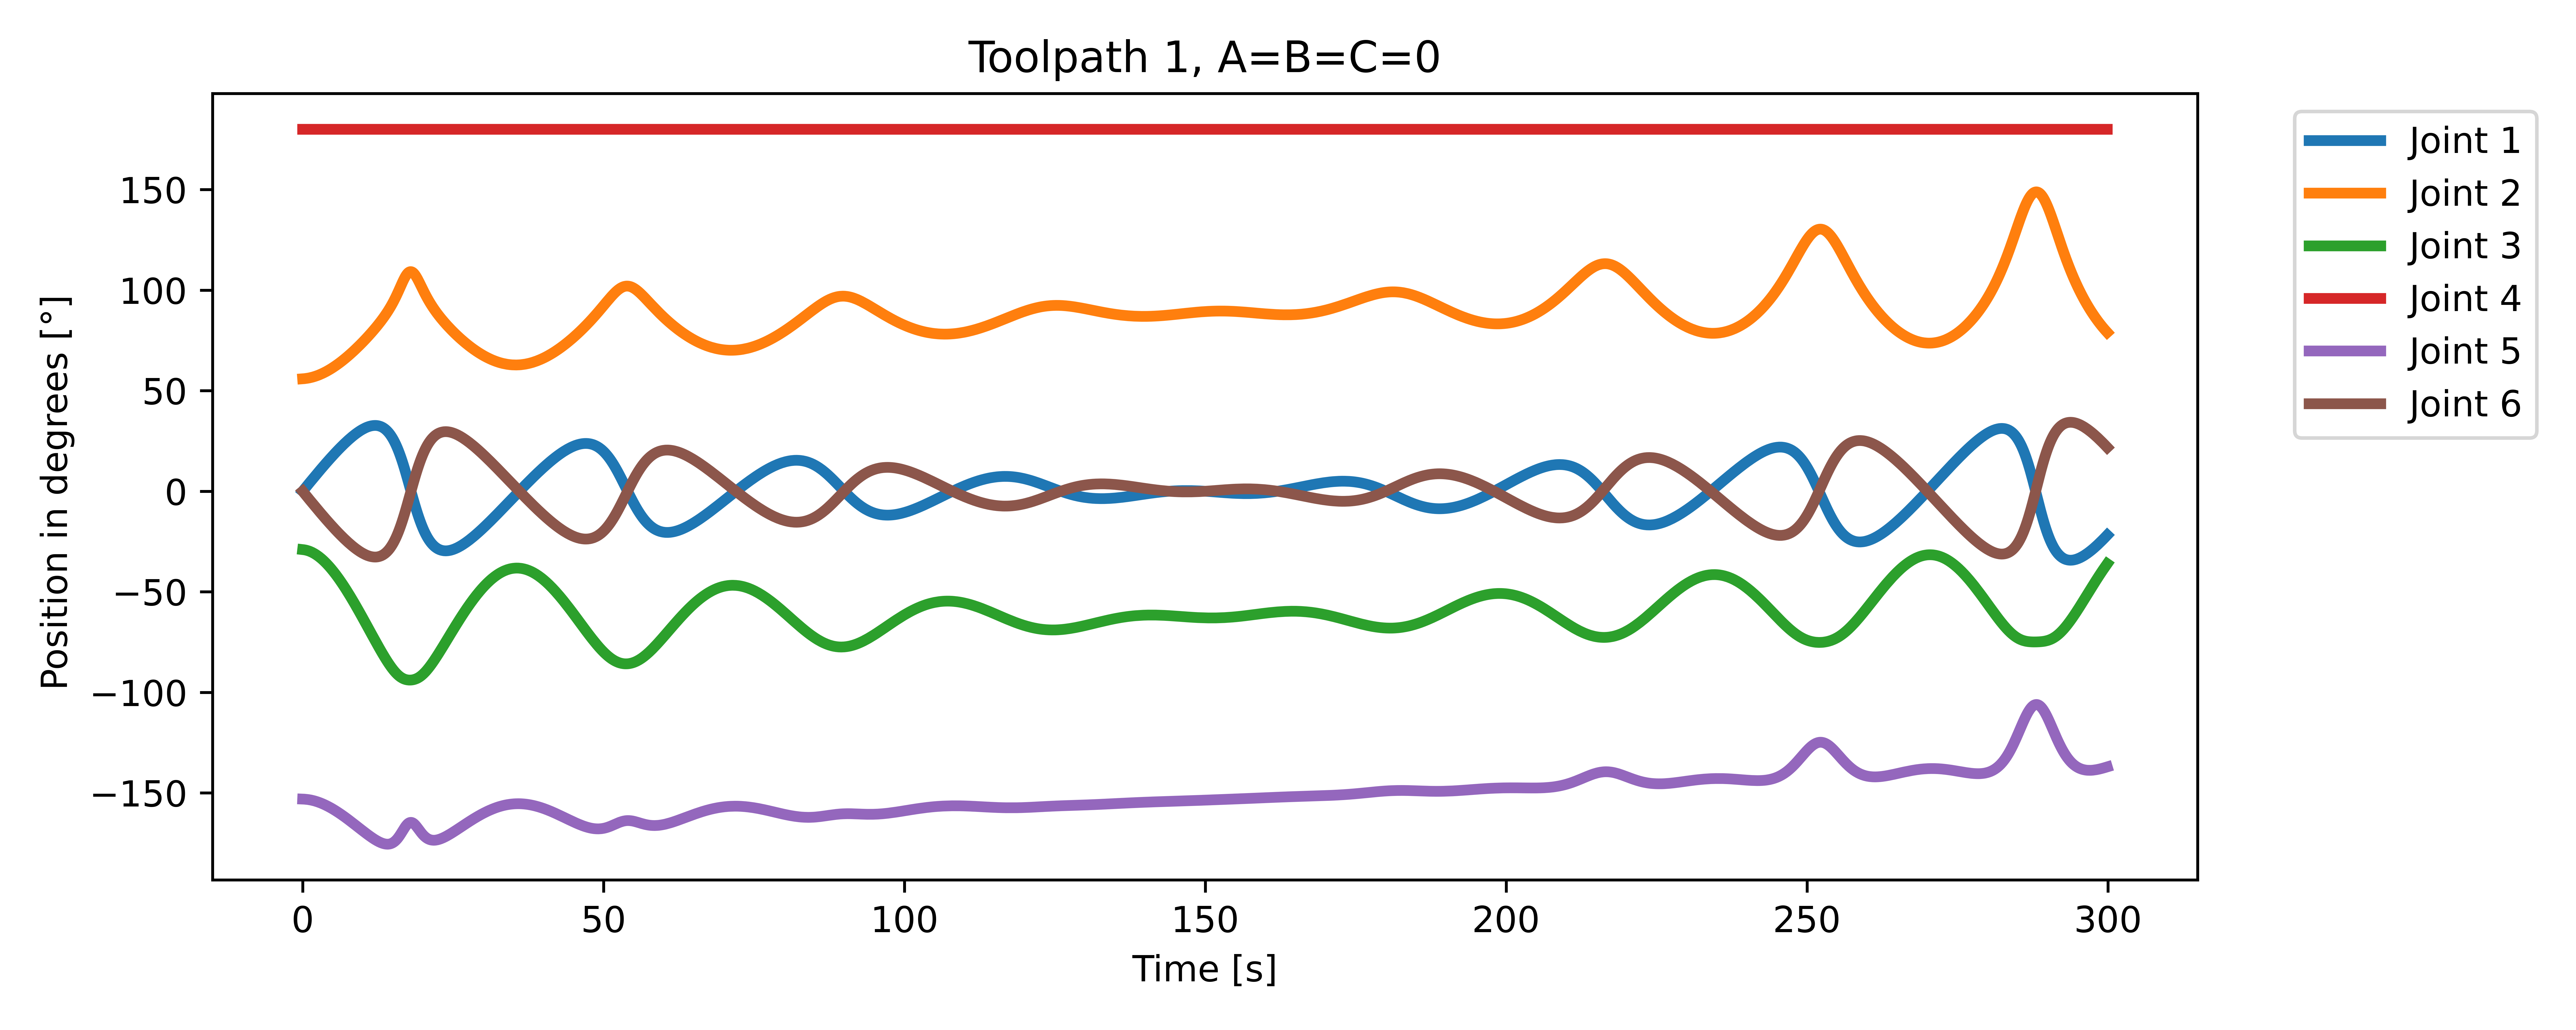
\includegraphics[width=1\textwidth]{figures/TP1ABC0.png}}
	\caption{Visualization of the joint positions over time for toolpath 1 with C=0°}
	\label{TP1ABC0}
\end{figure}

Figure \ref{TP1ABC45} depicts the joint positions for all six joints over time for the same toolpath (toolpath~1) with a 45° rotation around the Z-axis (C = 45°). 
\begin{figure}[H]
	\centerline{\includegraphics[width=1\textwidth]{figures/TP1ABC45.png}}
	\caption{Visualization of the joint positions over time for toolpath 1 with C=45°}
	\label{TP1ABC45}
\end{figure}
\newpage
It is noticeable that joint 4 and joint 5 have experienced changes in their respective ranges. Furthermore, joint 6 exhibits a significantly larger amplitude towards the end of the toolpath, in comparison to the case with no rotation (C=0°).

Figure \ref{TP1ABC0} illustrates the variations in each joint over time for toolpath 2 (Eq. \ref{eq2}) without any rotation (A=B=C=0°). Unlike toolpath 1, the amplitudes notably decrease towards the end of the toolpath. This observation aligns with the unique characteristics of different toolpaths.
 
 %In this case all joints show a oscillation except joint 4.
\begin{figure}[H]
	\centerline{\includegraphics[width=1\textwidth]{figures/TP2ABC0.png}}
	\caption{Visualization of the joint positions over time for toolpath 2}
	\label{TP2ABC0}
\end{figure}

%ToDo: EXPLAIN WHY JOINT 4 IS AT 180 all the time!!!!!!!!\newline
%\subsubsection{Selecting Process Parameters}
The next step involves selecting the process variables of interest and assigning weights to each variable. For this purpose, a basic case is discussed. The selected process variables are listed in Table \ref{PPbasic}. The total number of direction changes in all joints and the total distance traveled are chosen due to their ease of implementation. The number of direction changes is assigned an importance factor of 0.2.
The total travel in all joints is combined and given an importance factor of 0.4.
Additionally, the acceleration of joint 1 is analyzed. To obtain a scalar value for the acceleration, the individual acceleration values are squared and then summed up. The importance factor for acceleration in joint 1 is 0.4. Other process variables are disregarded.

\begin{table}[H]
	\centering
	\begin{tabular}{||l|l||}
		Process variables& Importance factors \\
		\hline
		\hline
		\hline
		Direction changes in joints 1-6	&		0.2 \\
		Total travel in joints 1-6	&  	0.4 \\
		Acceleration in joint 1	& 		0.4\\
		
		\hline
		\hline
	\end{tabular}
	
	\caption{Selected process variables and their importance factors}
	\label{PPbasic}
\end{table}


Since only one redundant \acrshort{DoF} is being analyzed, it is possible to represent the individual local scores and global score as a one-dimensional graph. Firstly, toolpath 1 is analyzed by incrementing the redundant \acrshort{DoF} (C-axis) by 5 degrees, starting from -135 degrees and ending at 135 degrees.


\newpage


Figure \ref{TP1-25} illustrates a case with a -45° rotation around the Z-axis for toolpath~1.
Similarly, Figure \ref{TP1+25} displays a case with a +45° rotation around the Z-axis for toolpath~1.

\begin{figure}[H]
	\centering
	\begin{minipage}{0.5\textwidth}
		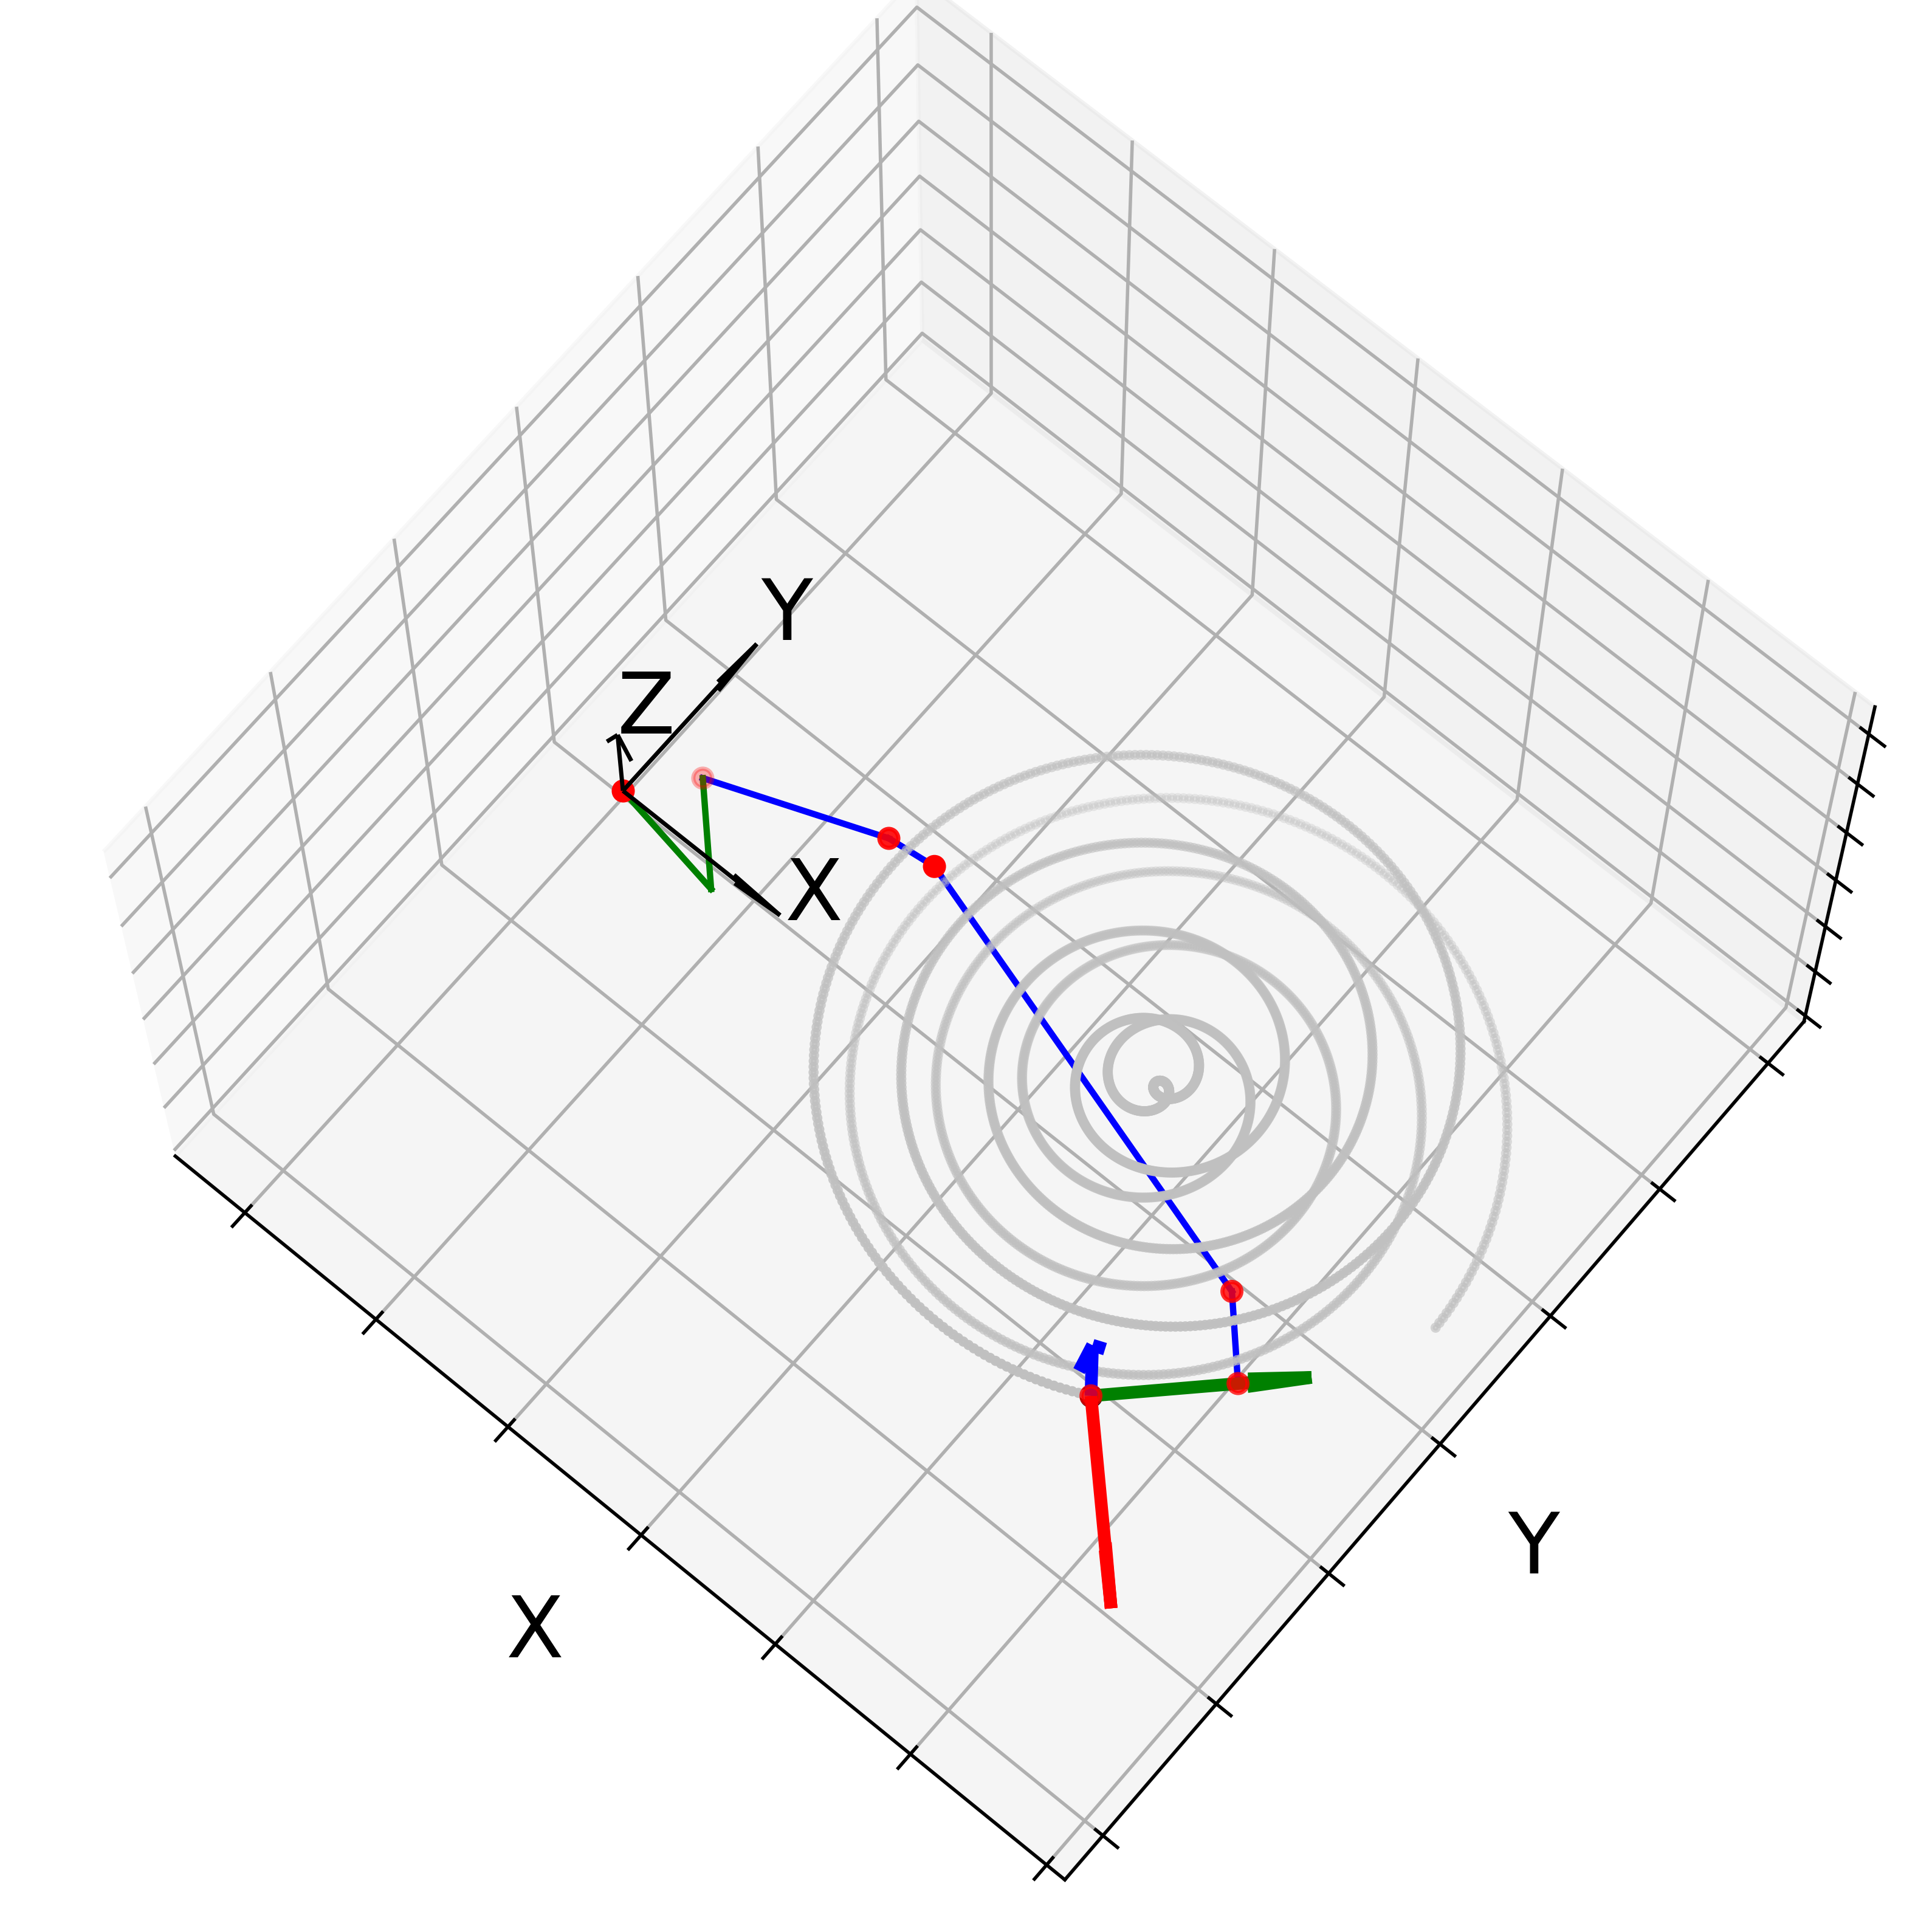
\includegraphics[width=\textwidth]{figures/robotANDpath1_-45.png}
		\caption{Toolpath 1 with A=0°, B=0° and C = -45°}
		\label{TP1-25}
	\end{minipage}\hfill
	\begin{minipage}{0.5\textwidth}
		\includegraphics[width=\textwidth]{figures/robotANDpath1_45.png}
		\caption{Toolpath 1 with A=0°, B=0° and C = 45°}
		\label{TP1+25}
	\end{minipage}\par
\end{figure}

A total of 55 time-series of joint positions are generated. On average, the inverse kinematics algorithm takes 35 seconds to calculate the joint values for all 3000 coordinates. The process variables are extracted and scaled in relation to each other, as described in Chapter~\ref{LRC}. It is important to note that before scaling, the selected process variables are pre-multiplied by -1, as each value should be minimized. The arrays of local ratings are then multiplied by the weights selected in Table \ref{PPbasic}. Subsequently, the local scores of each process variable can be plotted as a one-dimensional graph, as shown in Figure \ref{LS1}.

\begin{figure}[H]
	\centerline{
\includegraphics[width=1\textwidth]{figures/LocalScores_1.png}}
	\caption{Local scores of each process variable for toolpath 1}
	\label{LS1}
\end{figure}
\newpage
The acceleration in joint 1 and the combined total travel in the joints exhibit a smooth oscillating curve with a decreasing amplitude towards the positive end of the analyzed range. It is worth mentioning that the maximum value that the local score can reach is 40 for acceleration and total travel, while for direction changes, the maximum score is 20. This is due to the assigned importance factors. The direction changes display a less smooth, but still oscillating trajectory.

Next, the local scores are summed up to calculate the global score. The resulting array, displayed in Figure \ref{GS1}, represents the global score achieved by varying the rotation around the Z-axis in relation to all other analyzed values. The green cross on the graph indicates the maximum attainable score and its corresponding rotation, compared to all analyzed boundary conditions.

\begin{figure}[H]
	\centerline{\includegraphics[width=1\textwidth]{figures/best_c_1.png}}
	\caption{Global score for toolpath 1}
	\label{GS1}
\end{figure}
In this particular case, the highest achievable score is 91.1 at -120 degrees. This nearly perfect score indicates that setting the rotation to -120 degrees results in minimal direction changes, minimal total travel, and close to minimal acceleration in joint 1. It is crucial to emphasize that this rating is only in comparison to the other analyzed boundary conditions.

The same analysis, using identical process variables and weights, can be performed with toolpath 2 and toolpath 3. Figure \ref{TP2_combi} and Figure \ref{TP3_combi} display the global and local scores for each analyzed value of the redundant \acrshort{DoF}. For toolpath 2, the best score is 95.3 at -120 degrees, while for toolpath 3, the best score is 89.7 at -90 degrees.
\newpage

\begin{figure}[H]
\centerline{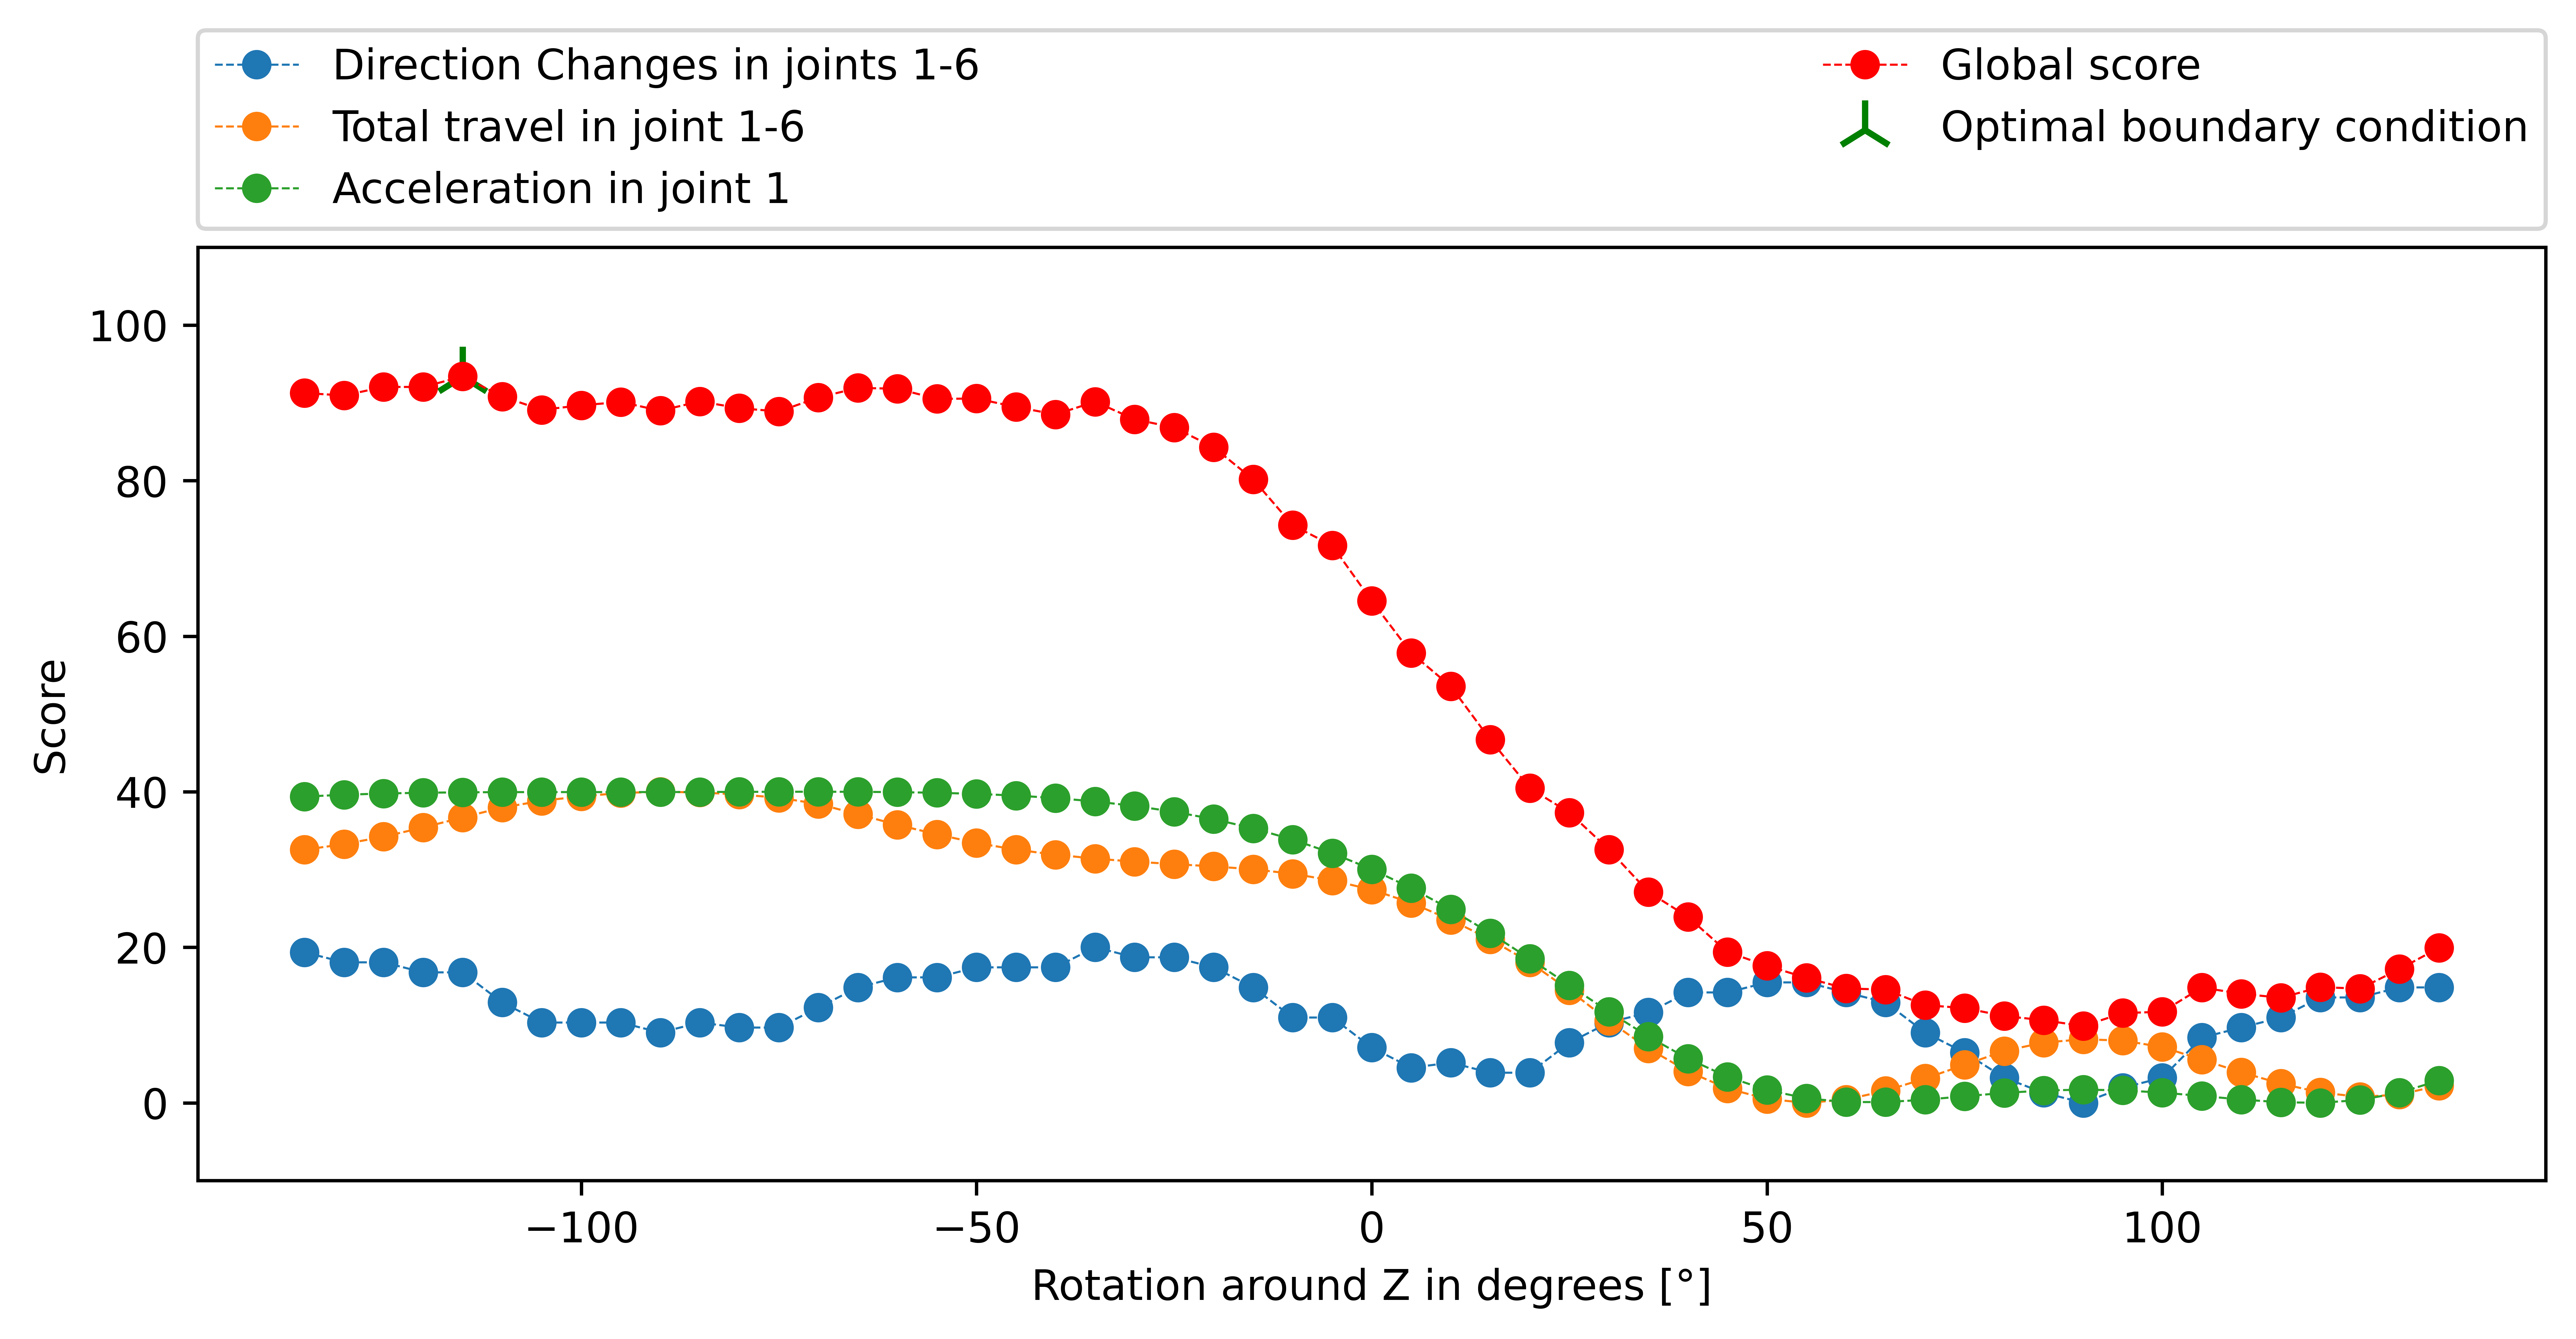
\includegraphics[width=1\textwidth]{figures/best_c_2_combi.png}}
\caption{Global and local scores in toolpath 2 depending on the rotation around Z}
\label{TP2_combi}
\end{figure}
\begin{figure}[H]
\centerline{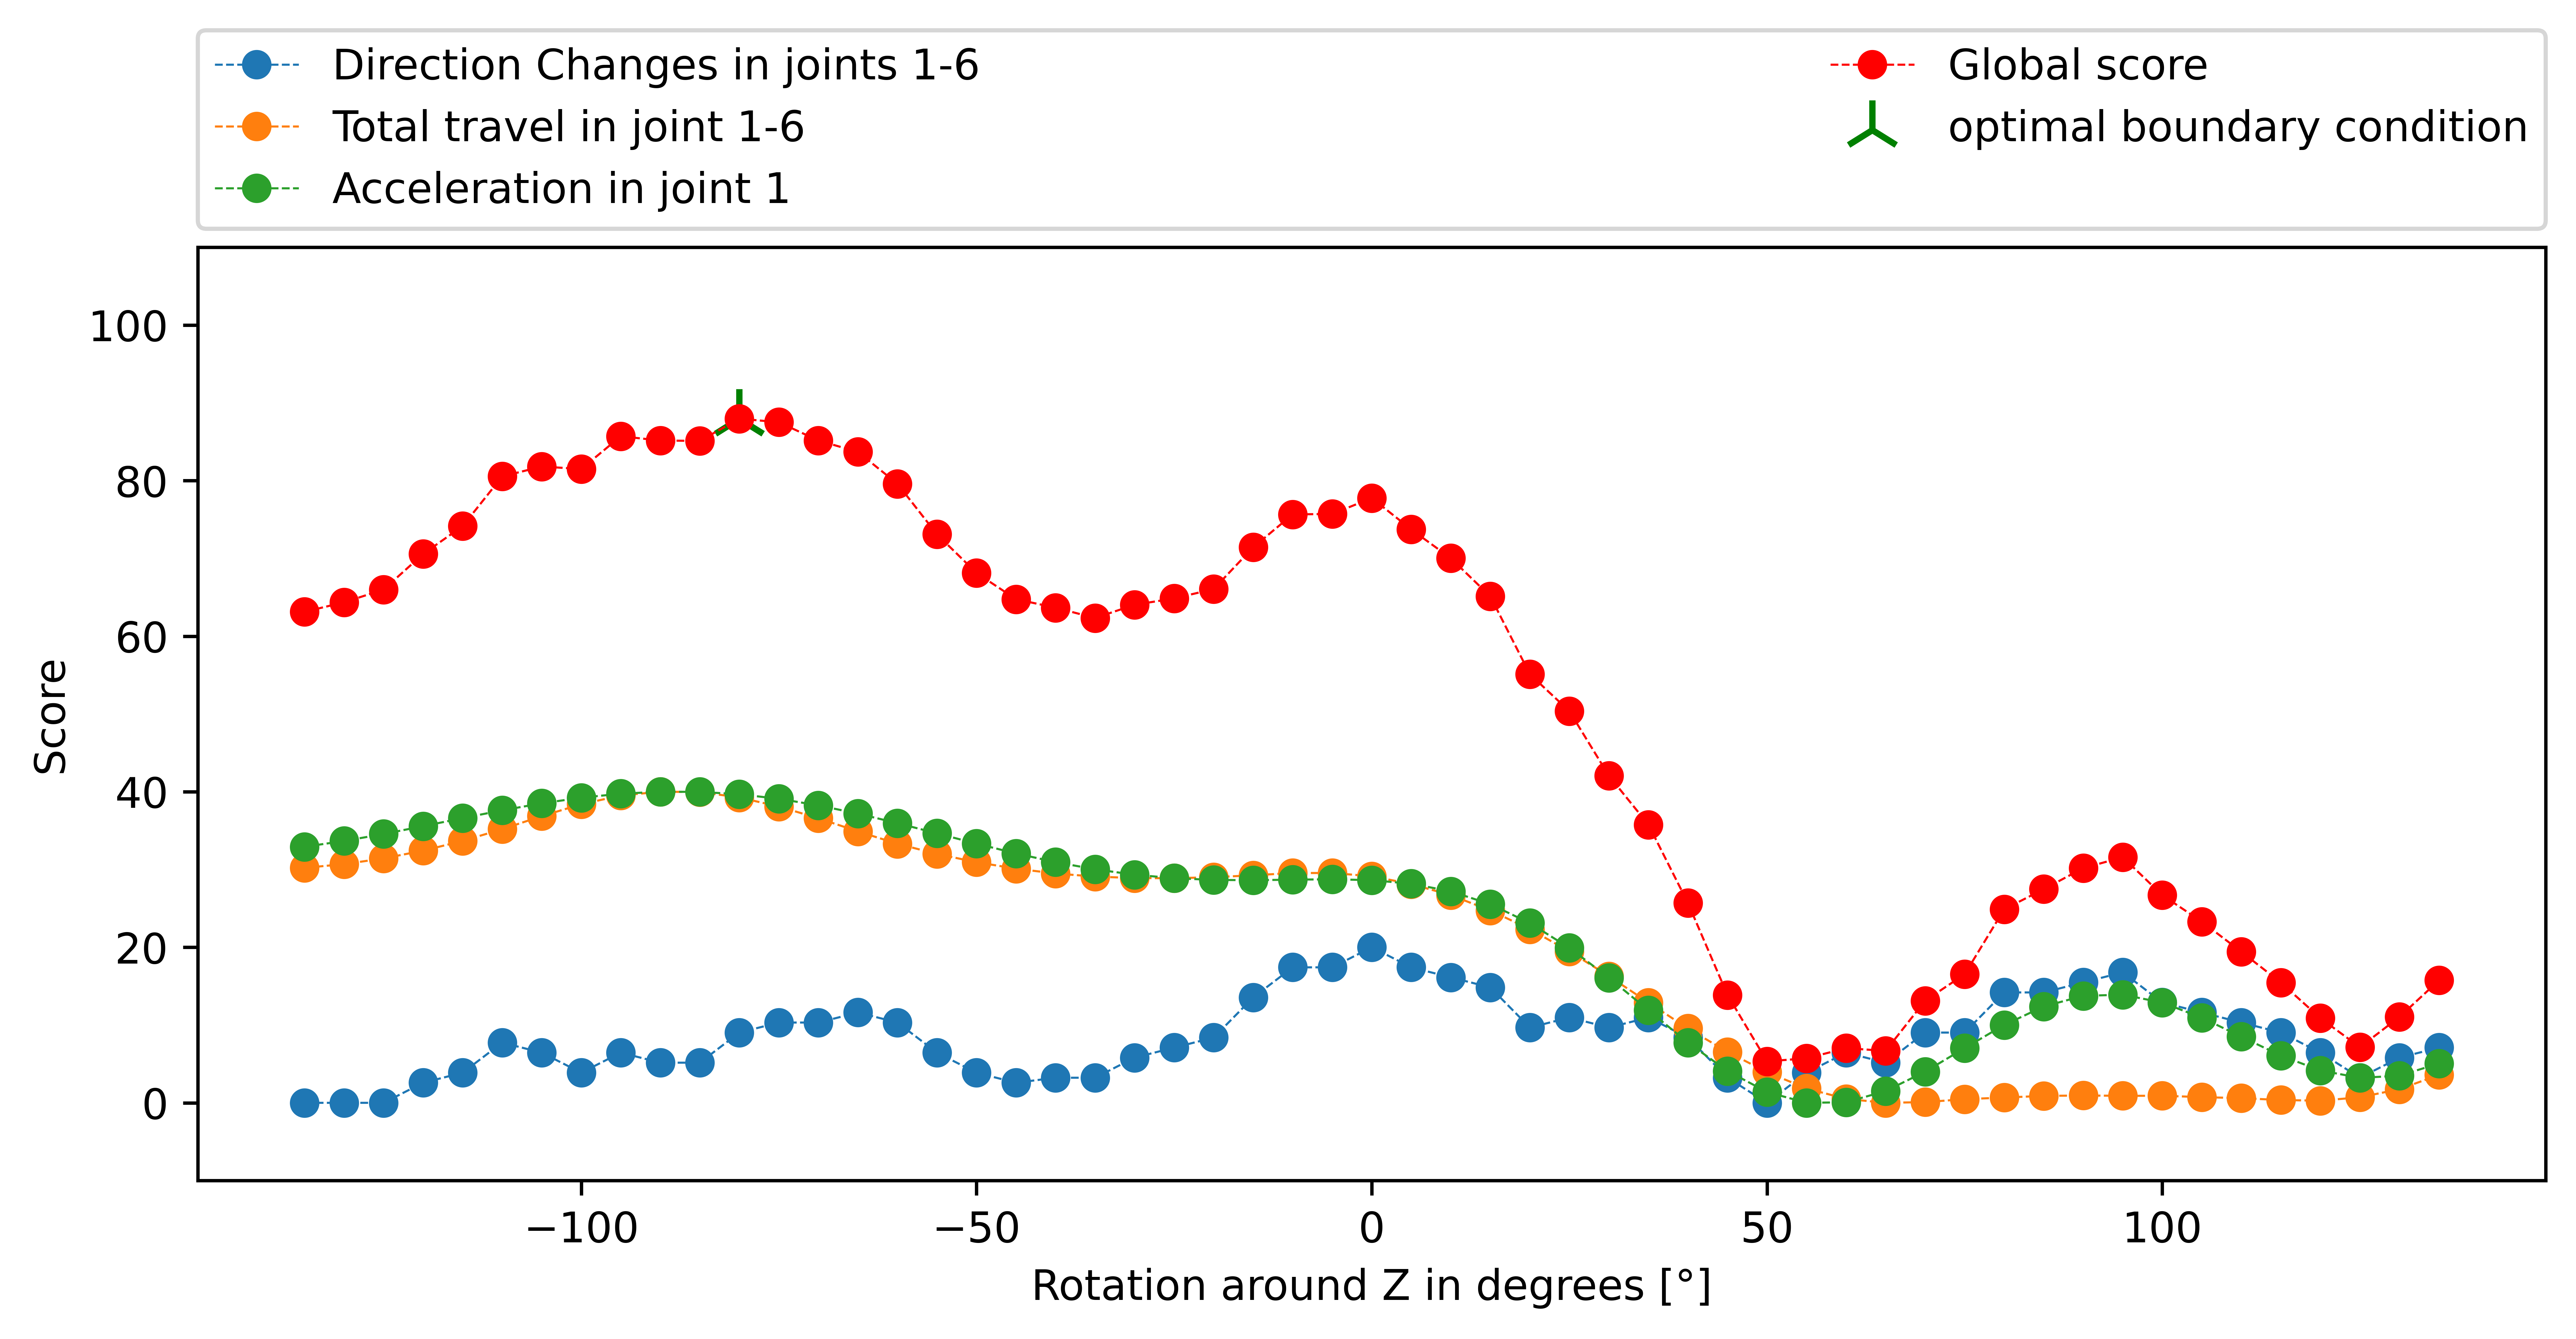
\includegraphics[width=1\textwidth]{figures/best_c_3_combi.png}}
\caption{Global and local scores in toolpath 3 depending on the rotation around Z}
\label{TP3_combi}
\end{figure}

It is noteworthy that even though all toolpaths have significantly different characteristics, all global scores show a similar trend. High global scores are achieved by setting the rotation to less than 0°, while low scores are achieved by setting the rotation to higher than 30°. Additionally, it is important to mention that when a local score reaches its maximum value, it does not imply that the corresponding process variables, such as the number of direction changes, become zero. Instead, it signifies that the number of direction changes is at its lowest compared to all other analyzed options.\newline
Based on this result, it is reasonable to conclude that correctly setting the redundant \acrshort{DoF}s can significantly improve the manufacturing process.
\newpage
\subsection{Validation on a Production Grade toolpath}\label{RG}
In addition to the three simulated toolpaths, a real toolpath used for \acrshort{WAAM} is now being used for validation. The toolpath has an organic structure that requires tilting of the rotary-tilt table to ensure that the material deposition process occurs in the direction of gravity. Thus, the position of the rotary-tilt table is not horizontal during the process. The redundant \acrshort{DoF} remains the rotation around the Z-axis of the tool, as before. Figure \ref{rav} provides a visual representation of the analyzed toolpath. It consists of 28,000 coordinates and is modeled to be traversed in 2,800 seconds.

\begin{figure}[H]
	\centerline{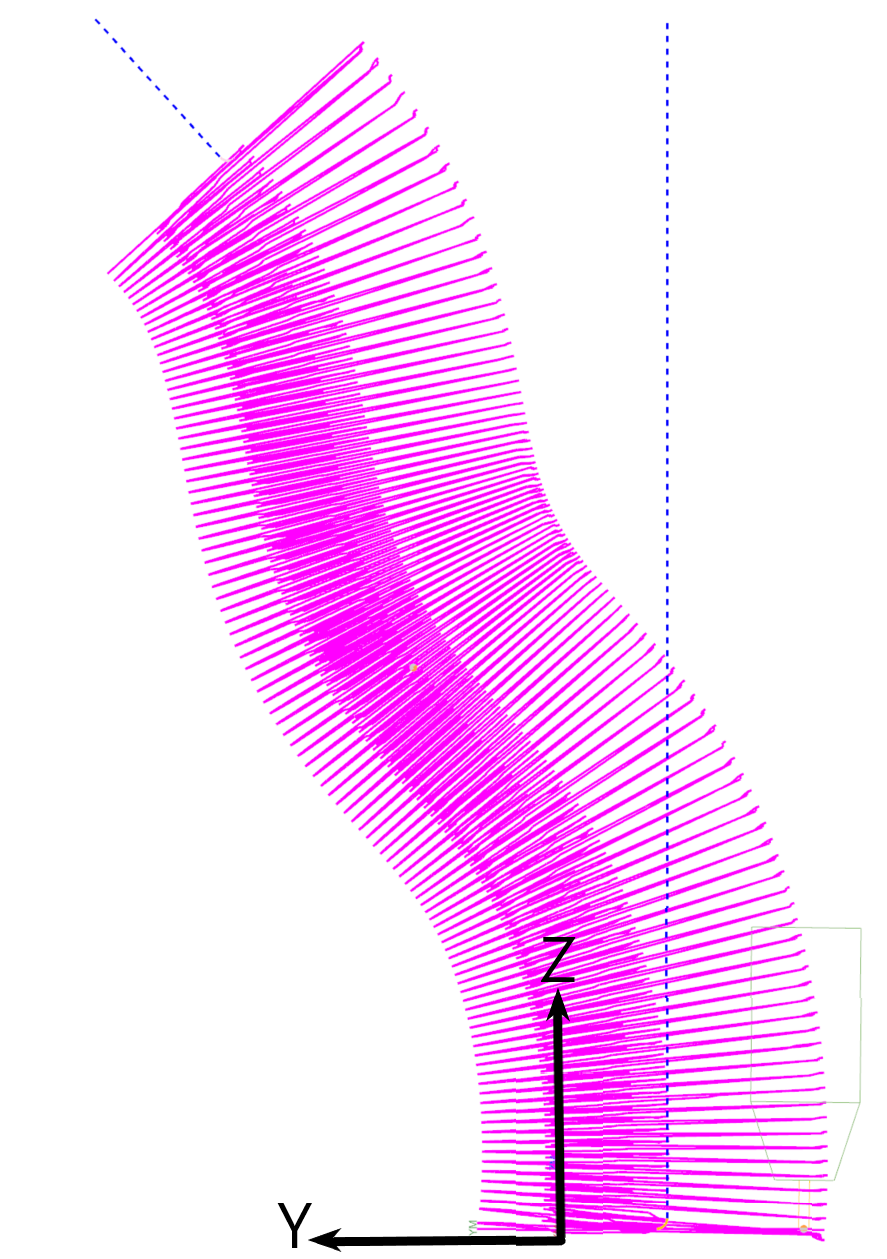
\includegraphics[width=0.3\textwidth]{figures/raven.png}}
	\caption{Organic toolpath \cite{Reisch.2023}}
	\label{rav}
\end{figure}

The process variables for the analysis of this toolpath are defined in Table \ref{ravenparams}. In this example, the direction changes in joints 1, 2, and 3 are all individually weighted with a factor of 0.2. The last two variables are the velocity in joint 5 and the total travel in joint 6. These variables are also weighted with an importance factor of 0.2. To obtain a scalar value for the velocity, all elements of the time-series are squared and summed up. 

\begin{table}[H]
	\centering
	\begin{tabular}{||l|l||}
		Process variables& Importance factors \\
		\hline
		\hline
		\hline
		Direction changes in joint 1	&		0.2 \\
		Direction changes in joint 2	&		0.2 \\
		Direction changes in joint 3	&		0.2 \\
		Velocity in joint 5	&		0.2 \\
		Total travel in joint 6	&		0.2 \\
		\hline
		\hline
	\end{tabular}
	
	\caption{Selected process variables and their importance factors for the organic toolpath}
	\label{ravenparams}
\end{table}

The redundant \acrshort{DoF} is once again analyzed in 5° increments, starting from -135° and ending at 135°. The resulting local scores are shown in Figure \ref{LS4}. It is evident that the velocity in joint 5 and the total travel in joint 6 exhibit a smooth oscillating behavior. The direction changes in joint 1 remain constant for all analyzed settings of the redundant \acrshort{DoF}. Therefore, the local score is set to 0 and is not further used in the calculation of the global score. The direction changes in joint 2 and 3 show a slight oscillation and exhibit a non-smooth progression towards the end and beginning of the analyzed range.

\begin{figure}[H]
	\centerline{\includegraphics[width=1\textwidth]{figures/LocalScores_4.png}}
	\caption{Global score for toolpath 1}
	\label{LS4}
\end{figure}

Figure \ref{GS4} illustrates the combined local scores in the form of the global score. The highest global score is 75.5, which is achieved by setting the C-axis to -15°. Notably, in the range from -70° to 40°, a very smooth curve is observed. This smooth progression of the global score serves as a strong indicator that an optimization algorithm will easily find an optimum setting for the redundant \acrshort{DoF}.

\begin{figure}[H]
	\centerline{\includegraphics[width=1\textwidth]{figures/best_c_4.png}}
	\caption{Global score for production toolpath}
	\label{GS4}
\end{figure}


\newpage

\subsection{Toolpath Evaluation With two Redundant DoF}\label{2RDOF}

To introduce an additional redundant \acrshort{DoF}, a rotary-tilt table is simulated. Currently, only the tilting aspect is being analyzed. All coordinates of the toolpath can be rotated by a specified degree around the X-axis of the toolpath coordinate system. Figure \ref{TP3_0} depicts toolpath 3 with no rotation around the X-axis, while Figure \ref{TP3_25} illustrates a rotation of +25 degrees.

\begin{figure}[H]% [H] is so declass\'e!
	\centering
	\begin{minipage}{0.5\textwidth}
		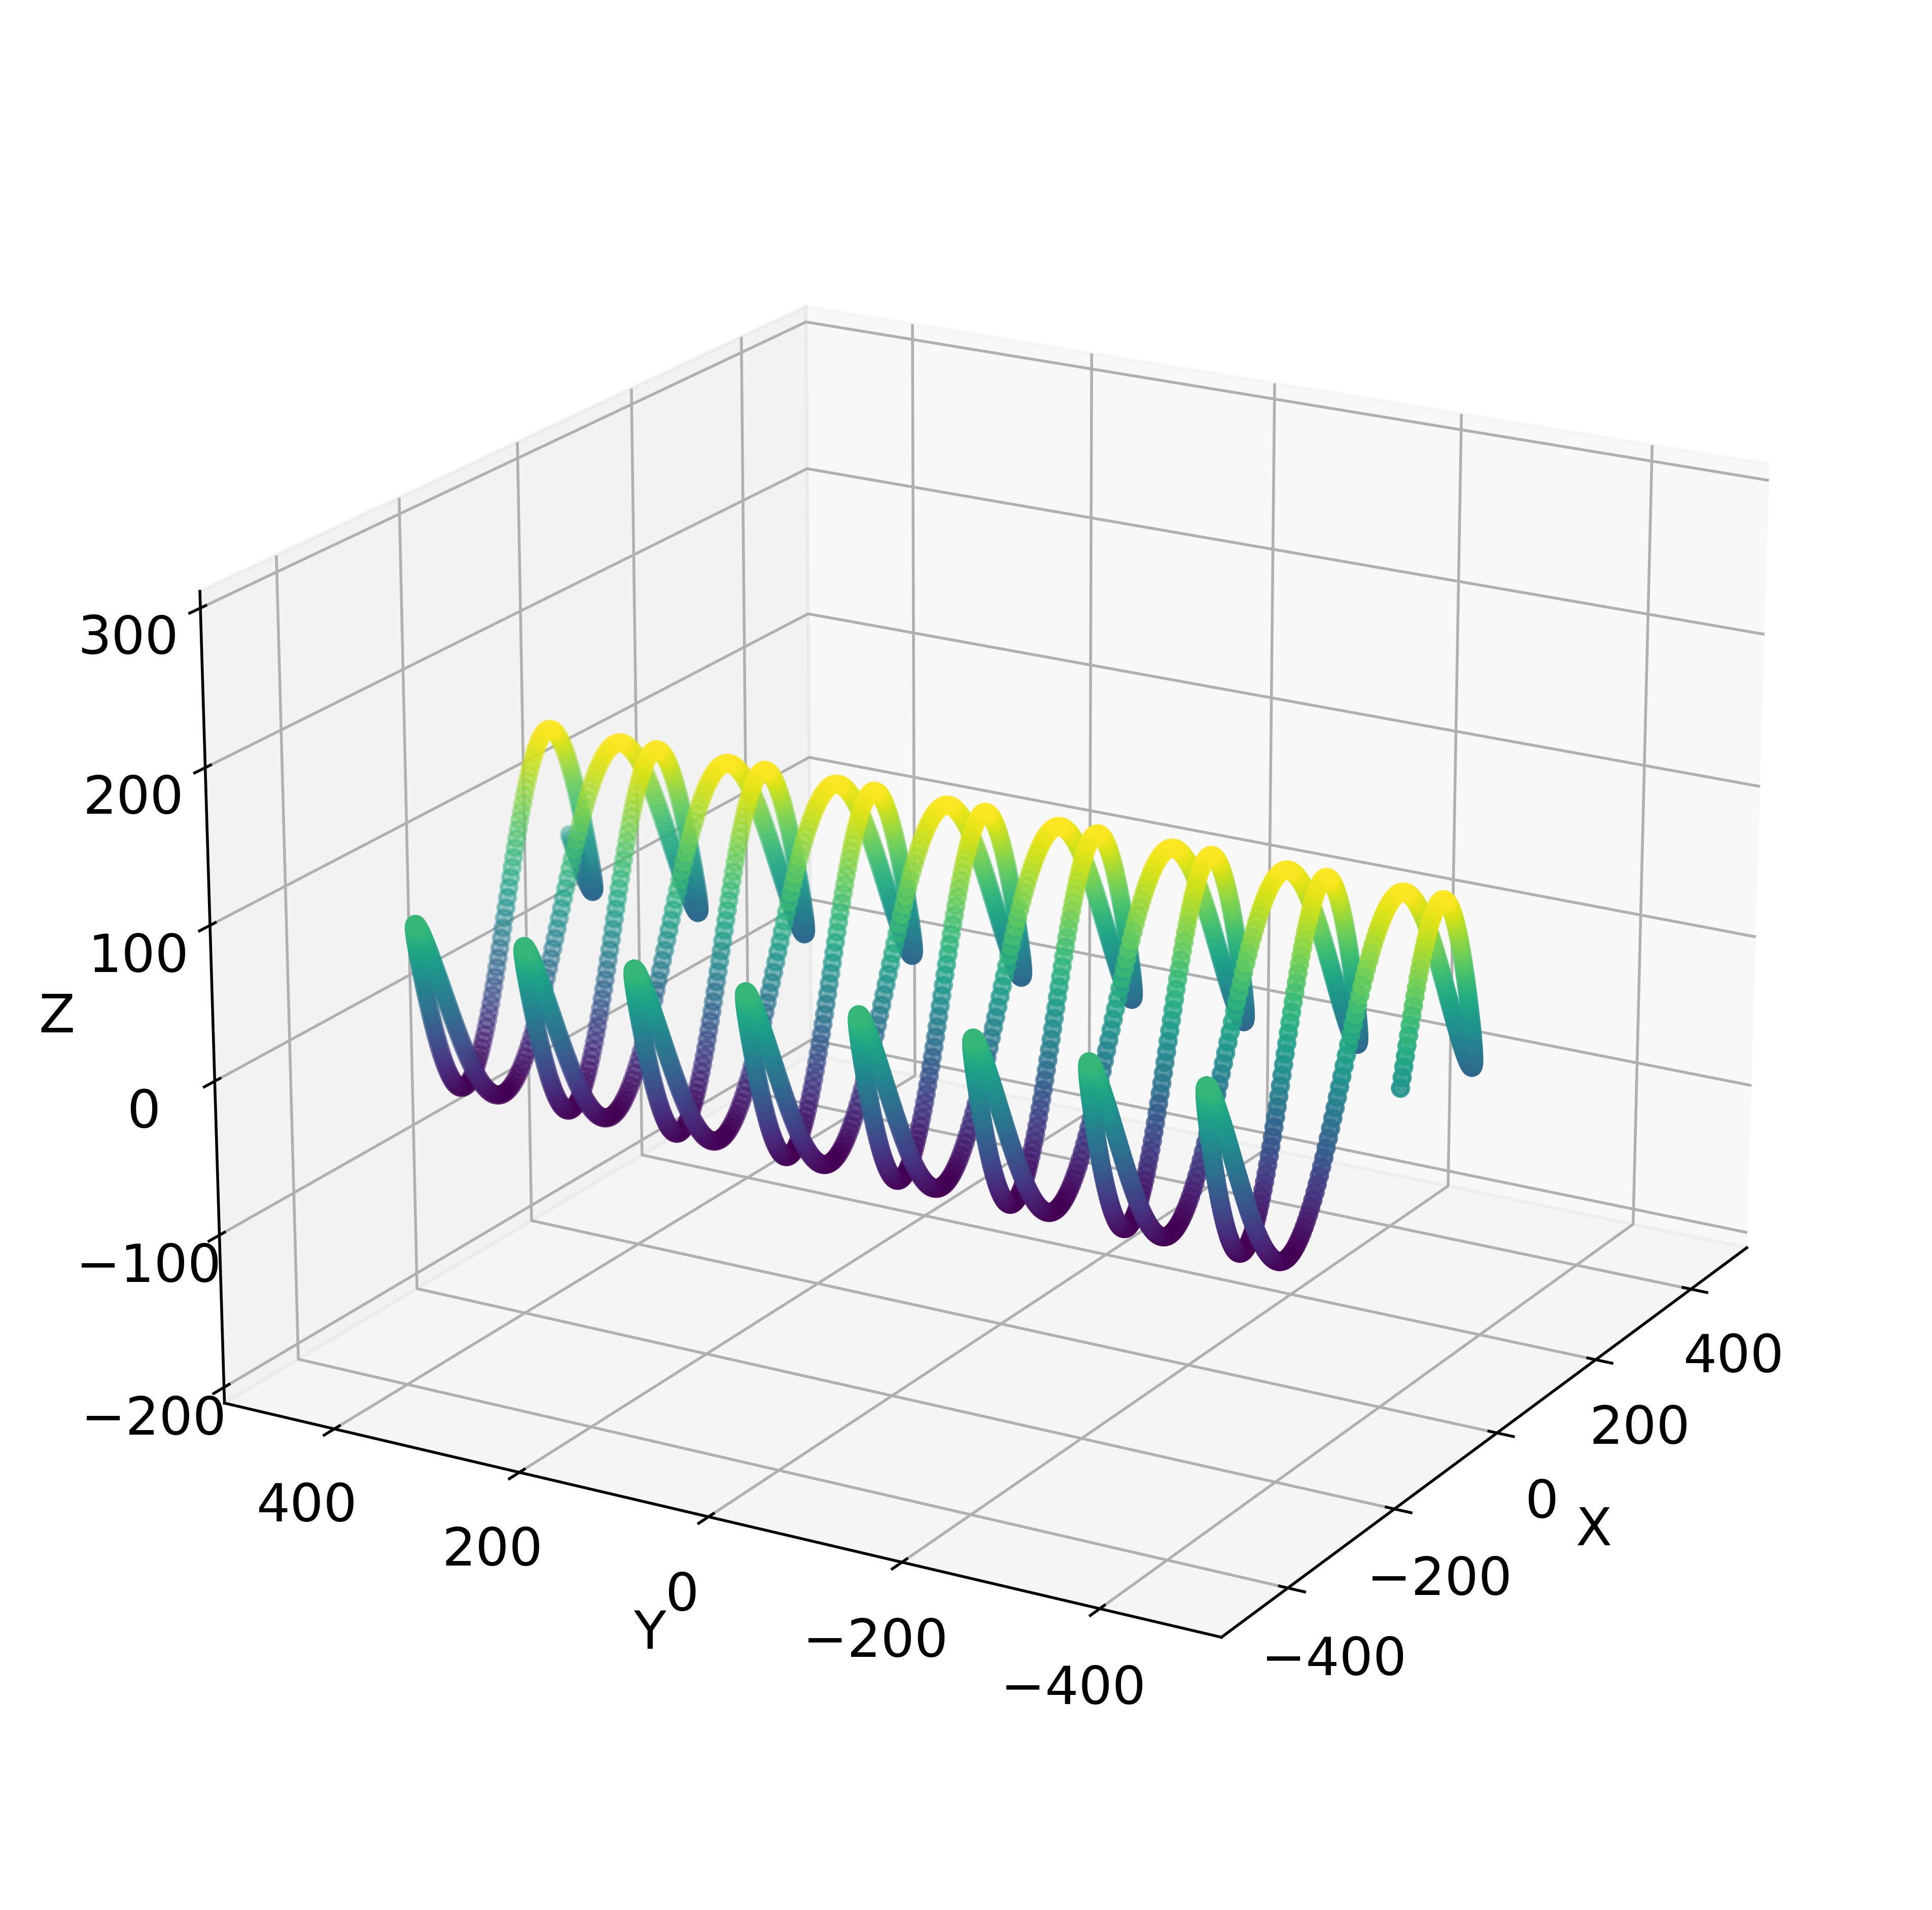
\includegraphics[width=\textwidth]{figures/path3_kipp_0.png}
		\caption{Toolpath 3 with no rotation\newline around the X-axis}
		\label{TP3_0}
	\end{minipage}\hfill
	\begin{minipage}{0.5\textwidth}
		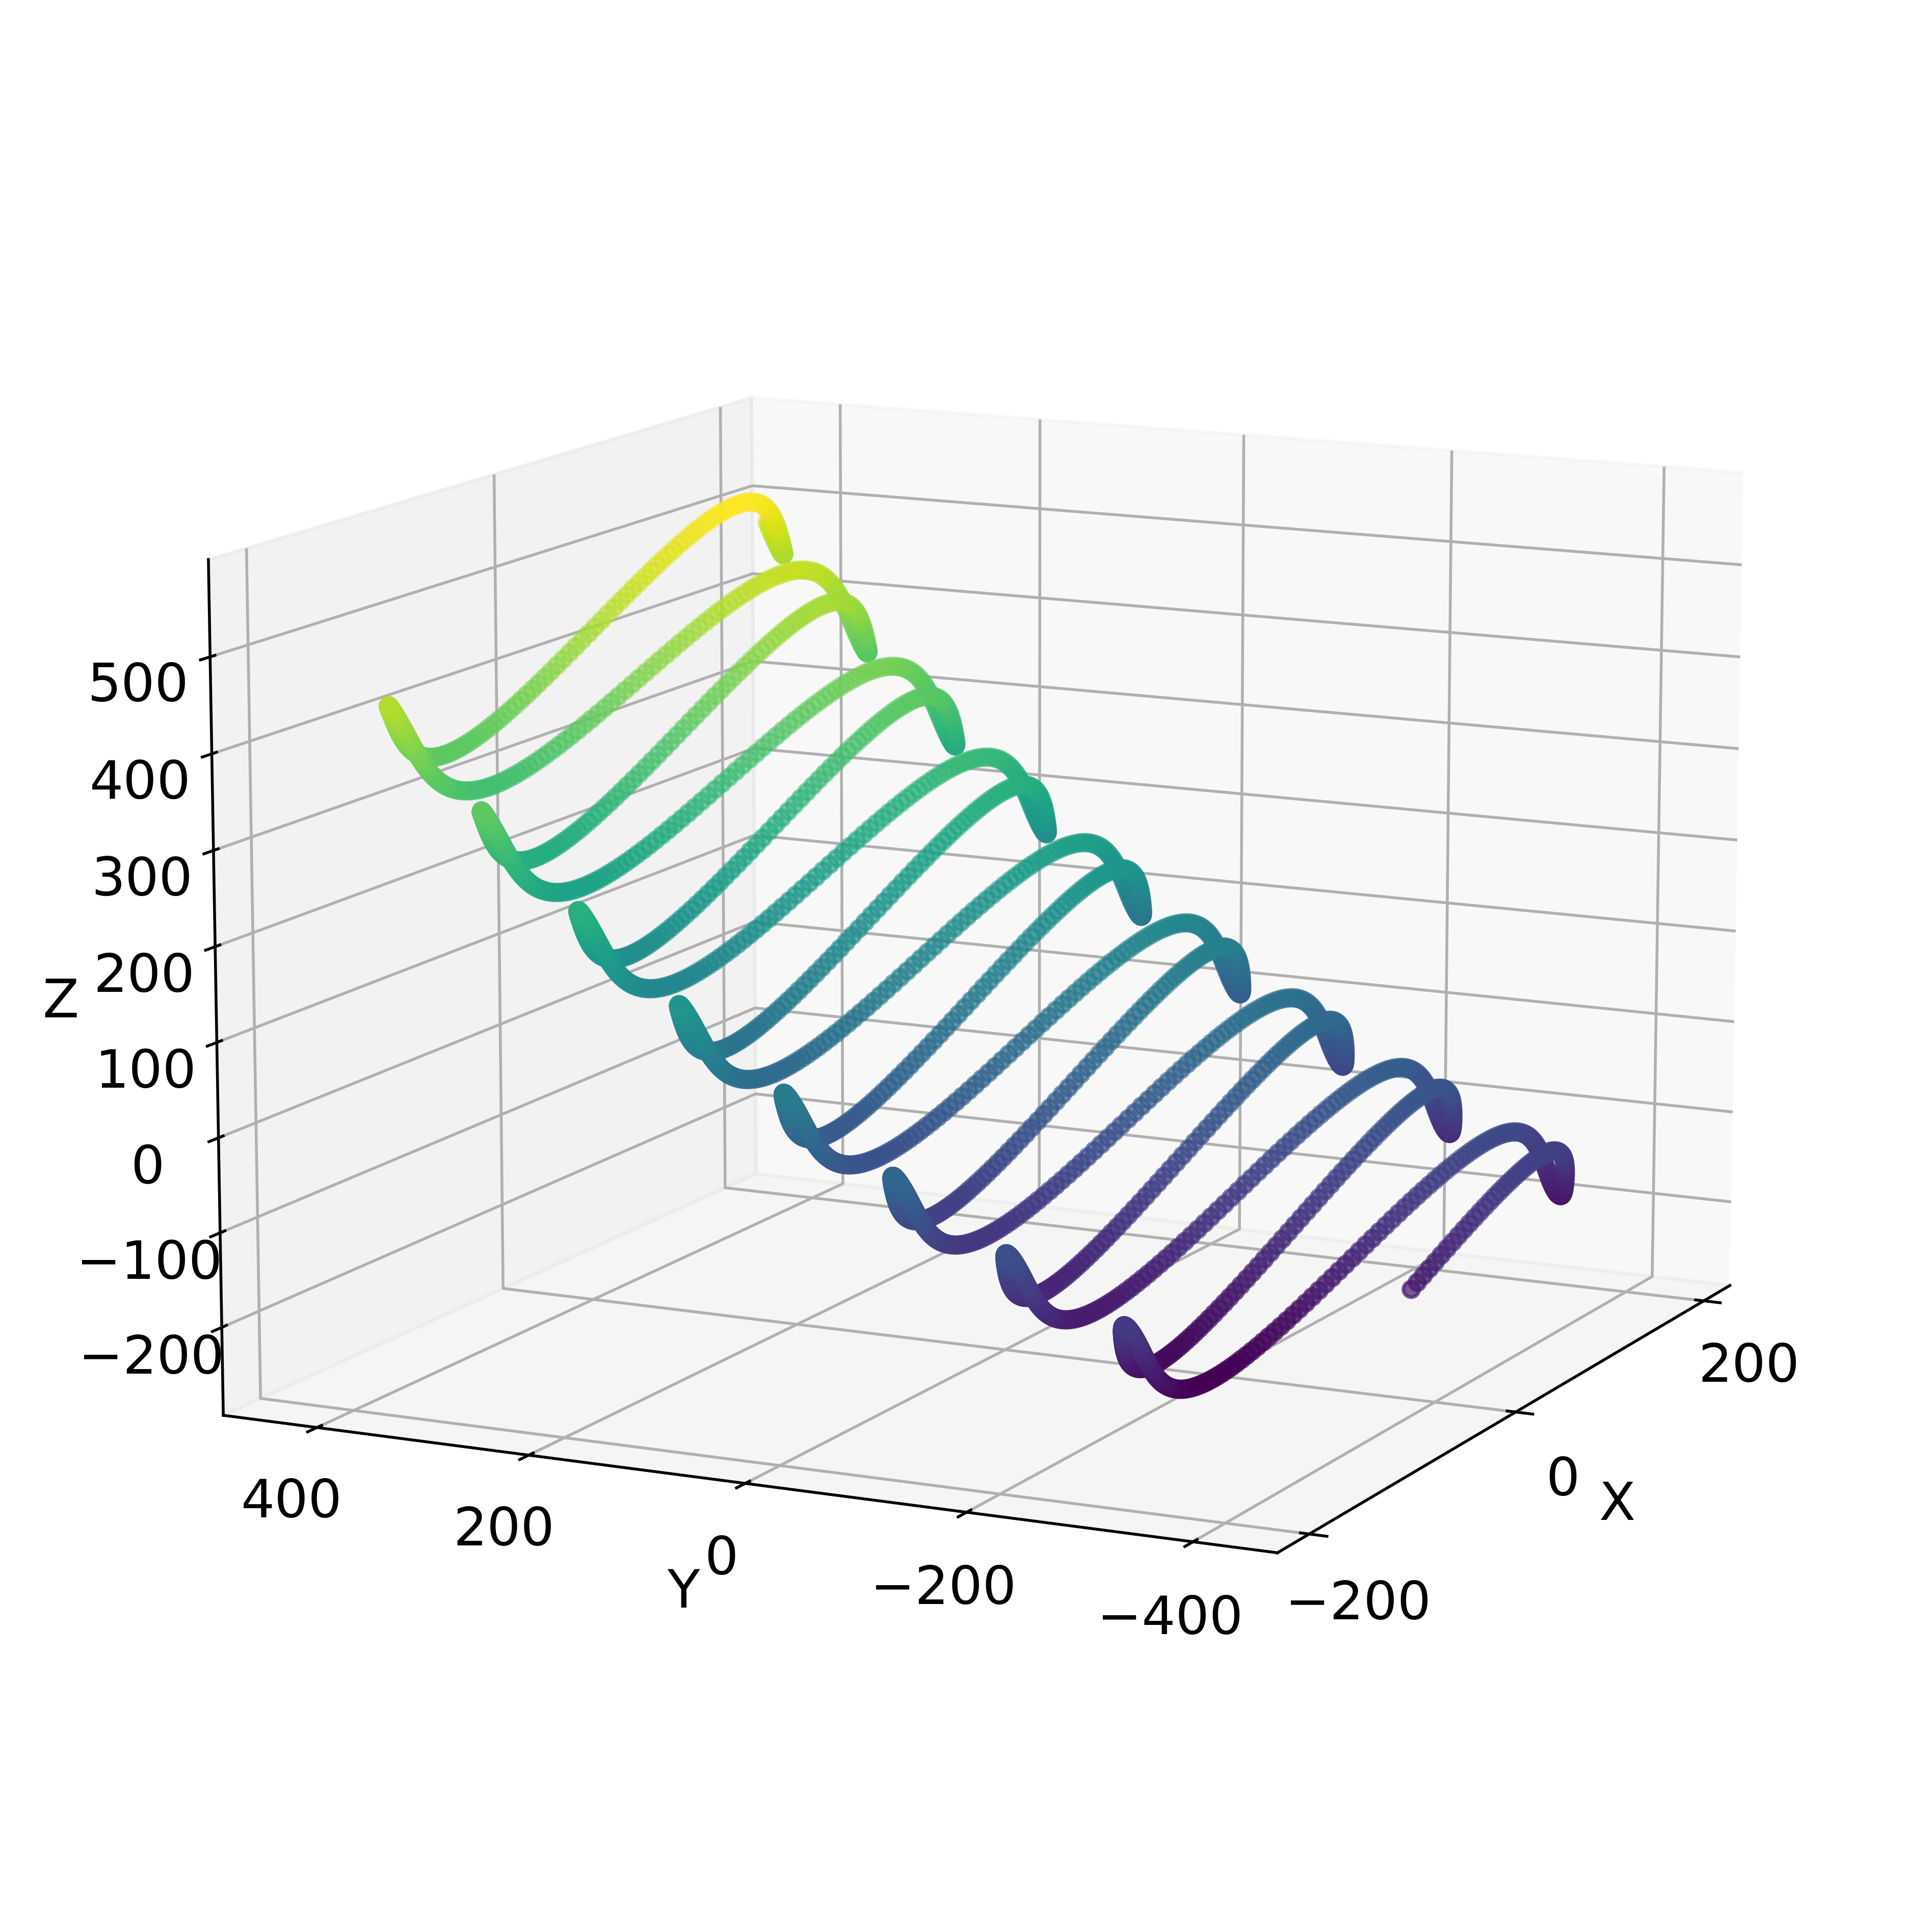
\includegraphics[width=\textwidth]{figures/path3_kipp_25_comparison.png}
		\caption{Toolpath 3 with a rotation\newline of 25 degrees around the X-axis}
		\label{TP3_25}
	\end{minipage}\par
\end{figure}
 

Similar to the previous analysis, the same steps need to be followed. The newly selected process variables are presented in Table \ref{PP_2}. The direction changes of the tilting joints (2+3+5) are combined and treated as one process variable, weighted with a factor of 0.3. Direction changes in joint 1 and acceleration in joint 4 are considered as individual variables, both individually weighted with 0.25. The final variable is the velocity in joint 6, weighted with 0.2.

\begin{table}[H]
	\centering
	\begin{tabular}{||l|l||}
		Process variables & Importance factors \\
		\hline
		\hline
		\hline
		Direction changes in joints 2+3+5	&		0.3 \\
		Direction changes in joints 1	& 	0.25 \\
		Acceleration in joint 4	& 		0.25\\
		Velocity in joint 6	& 		0.2\\
		\hline
		\hline
	\end{tabular}
	
	\caption{Selected process variables and their importance factors for 2 redundant DoF}
	\label{PP_2}
\end{table}


Figure \ref{TP3_25_robot} displays the robot and its orientation while following the tilted toolpath 3. It is crucial to note that since the toolpath is defined in 5 \acrshort{DoF}s in its own frame, the frame of the \acrshort{TCP} must also tilt by the same degree as the table. The two redundant \acrshort{DoF}s in this case are the rotation around the Z-axis in the frame of the tilted toolpath and the tilting of the toolpath itself. This introduces an additional dimension, as now two parameters can be adapted for optimization.


\begin{figure}[H]
	\centerline{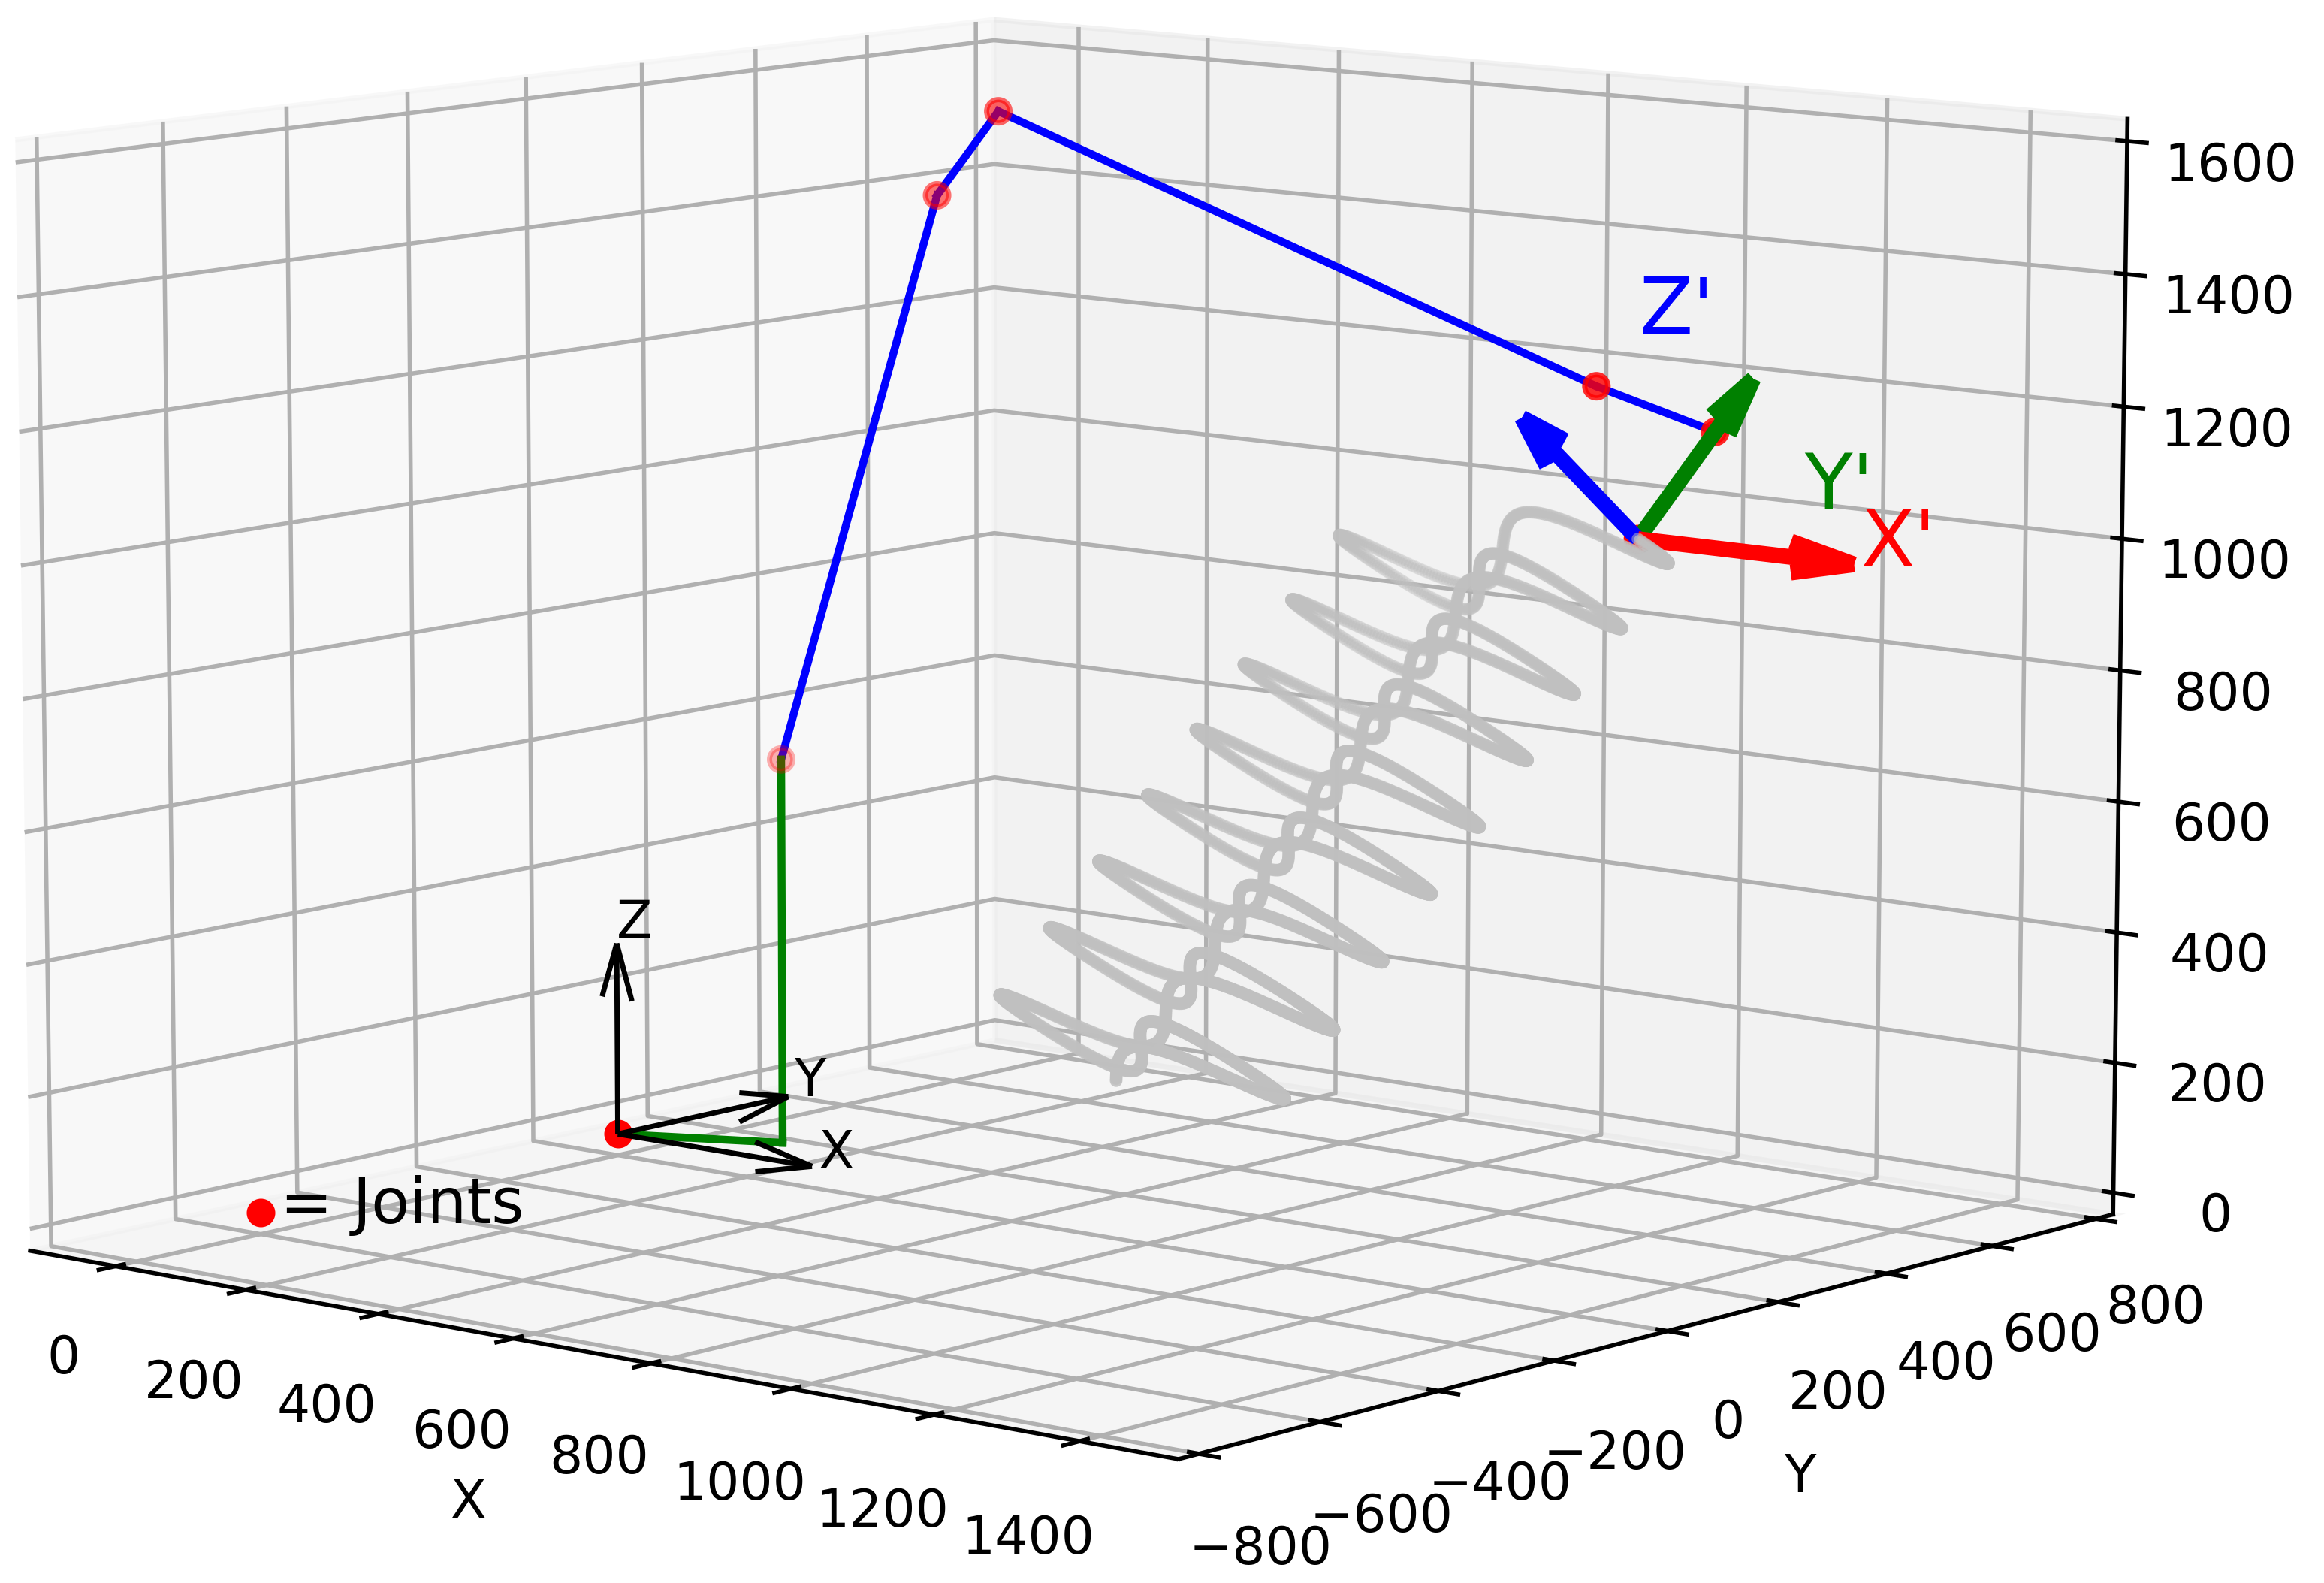
\includegraphics[width=0.9\textwidth]{figures/robotANDpath3_45.png}}
	\caption{Robot following the tilted toolpath 3}
	\label{TP3_25_robot}
\end{figure}

The range of possible tilt positions ranges from -45° to 45° in 2-degree increments. For every combination of tilt and rotation, the joint angles are generated using inverse kinematics. To speed up the computation, only every third coordinate is utilized in the inverse kinematic algorithm. This reduces the toolpath by 2000 points and speeds up calculation time. On average, it now takes only 10 seconds to calculate the joint positions. A total of 2530 individual combinations are analyzed.

The extracted process variables are again multiplied by -1, as the objective is to minimize them. Afterwards, the Min-Max scaler is applied. The individual values are aggregated and presented in the form of a matrix. The values of this matrix are visualized in Figure \ref{best_2D}. The maximum achievable score from all possible combinations is 70.4, visualized by the red cross. This score was attained by setting the table tilt to -5° and the rotation around the Z-axis of the tool to +35°. The resulting hyperplane exhibits two distinct local maxima. The entire surface displays a smooth curvature, although it appears less smooth in the range from -20° to 45°.


\begin{figure}[H]
	\centerline{\includegraphics[width=1\textwidth]{figures/best_2D_3.png}}
	\caption{Hyperplane representing the global score of toolpath 3}
	\label{best_2D}
\end{figure}

The same analysis is performed with toolpath 1 and toolpath 2. The resulting matrix of the global scores for each possible boundary condition combination is shown in Figure \ref{best_2D_1} and Figure \ref{best_2D_2}, respectively. The same process variables and weights (see Table \ref{PP_2}) are used for the calculations.
\newpage

\begin{figure}[H]
	\centerline{\includegraphics[width=0.7\textwidth]{figures/best_2D_1.png}}
	\caption{Hyperplane representing the global score of toolpath 1}
	\label{best_2D_1}
\end{figure}

\begin{figure}[H]
	\centerline{\includegraphics[width=0.7\textwidth]{figures/best_2D_2.png}}
	\caption{Hyperplane representing the global score of toolpath 2}
	\label{best_2D_2}
\end{figure}


\newpage
\subsection{Boundary Condition Optimization }
So far, only the analysis of different boundary conditions has been performed by exploring the entire range of possible settings for the redundant \acrshort{DoF}s. However, this approach is very time-consuming and becomes exponentially more complex with additional redundant \acrshort{DoF} and a finer step size. To address this issue and efficiently search the extensive solution space for optimal values of the redundant \acrshort{DoF}, a \acrshort{PSO} algorithm is proposed. In this algorithm, individual particles navigate the search space by adjusting their positions based on their own best position and the best position found by the entire swarm. This cooperative behavior enables the particles to explore the search space more effectively and converge towards the best solution (see Chapter \ref{OA}).

The first test is conducted using the global score matrix of toolpath 3. Initially, 20 particles are randomly placed on the plane. Each particle's score is determined by the corresponding global score at its position. By increasing the number of particles and iterations, the search space can be analyzed more comprehensively. Figure \ref{PSO_1} illustrates the randomly placed particles on the pre-calculated global score matrix of toolpath 3, considering the previously selected importance factors (see table \ref{PP_2}).

\begin{figure}[H]
	\centerline{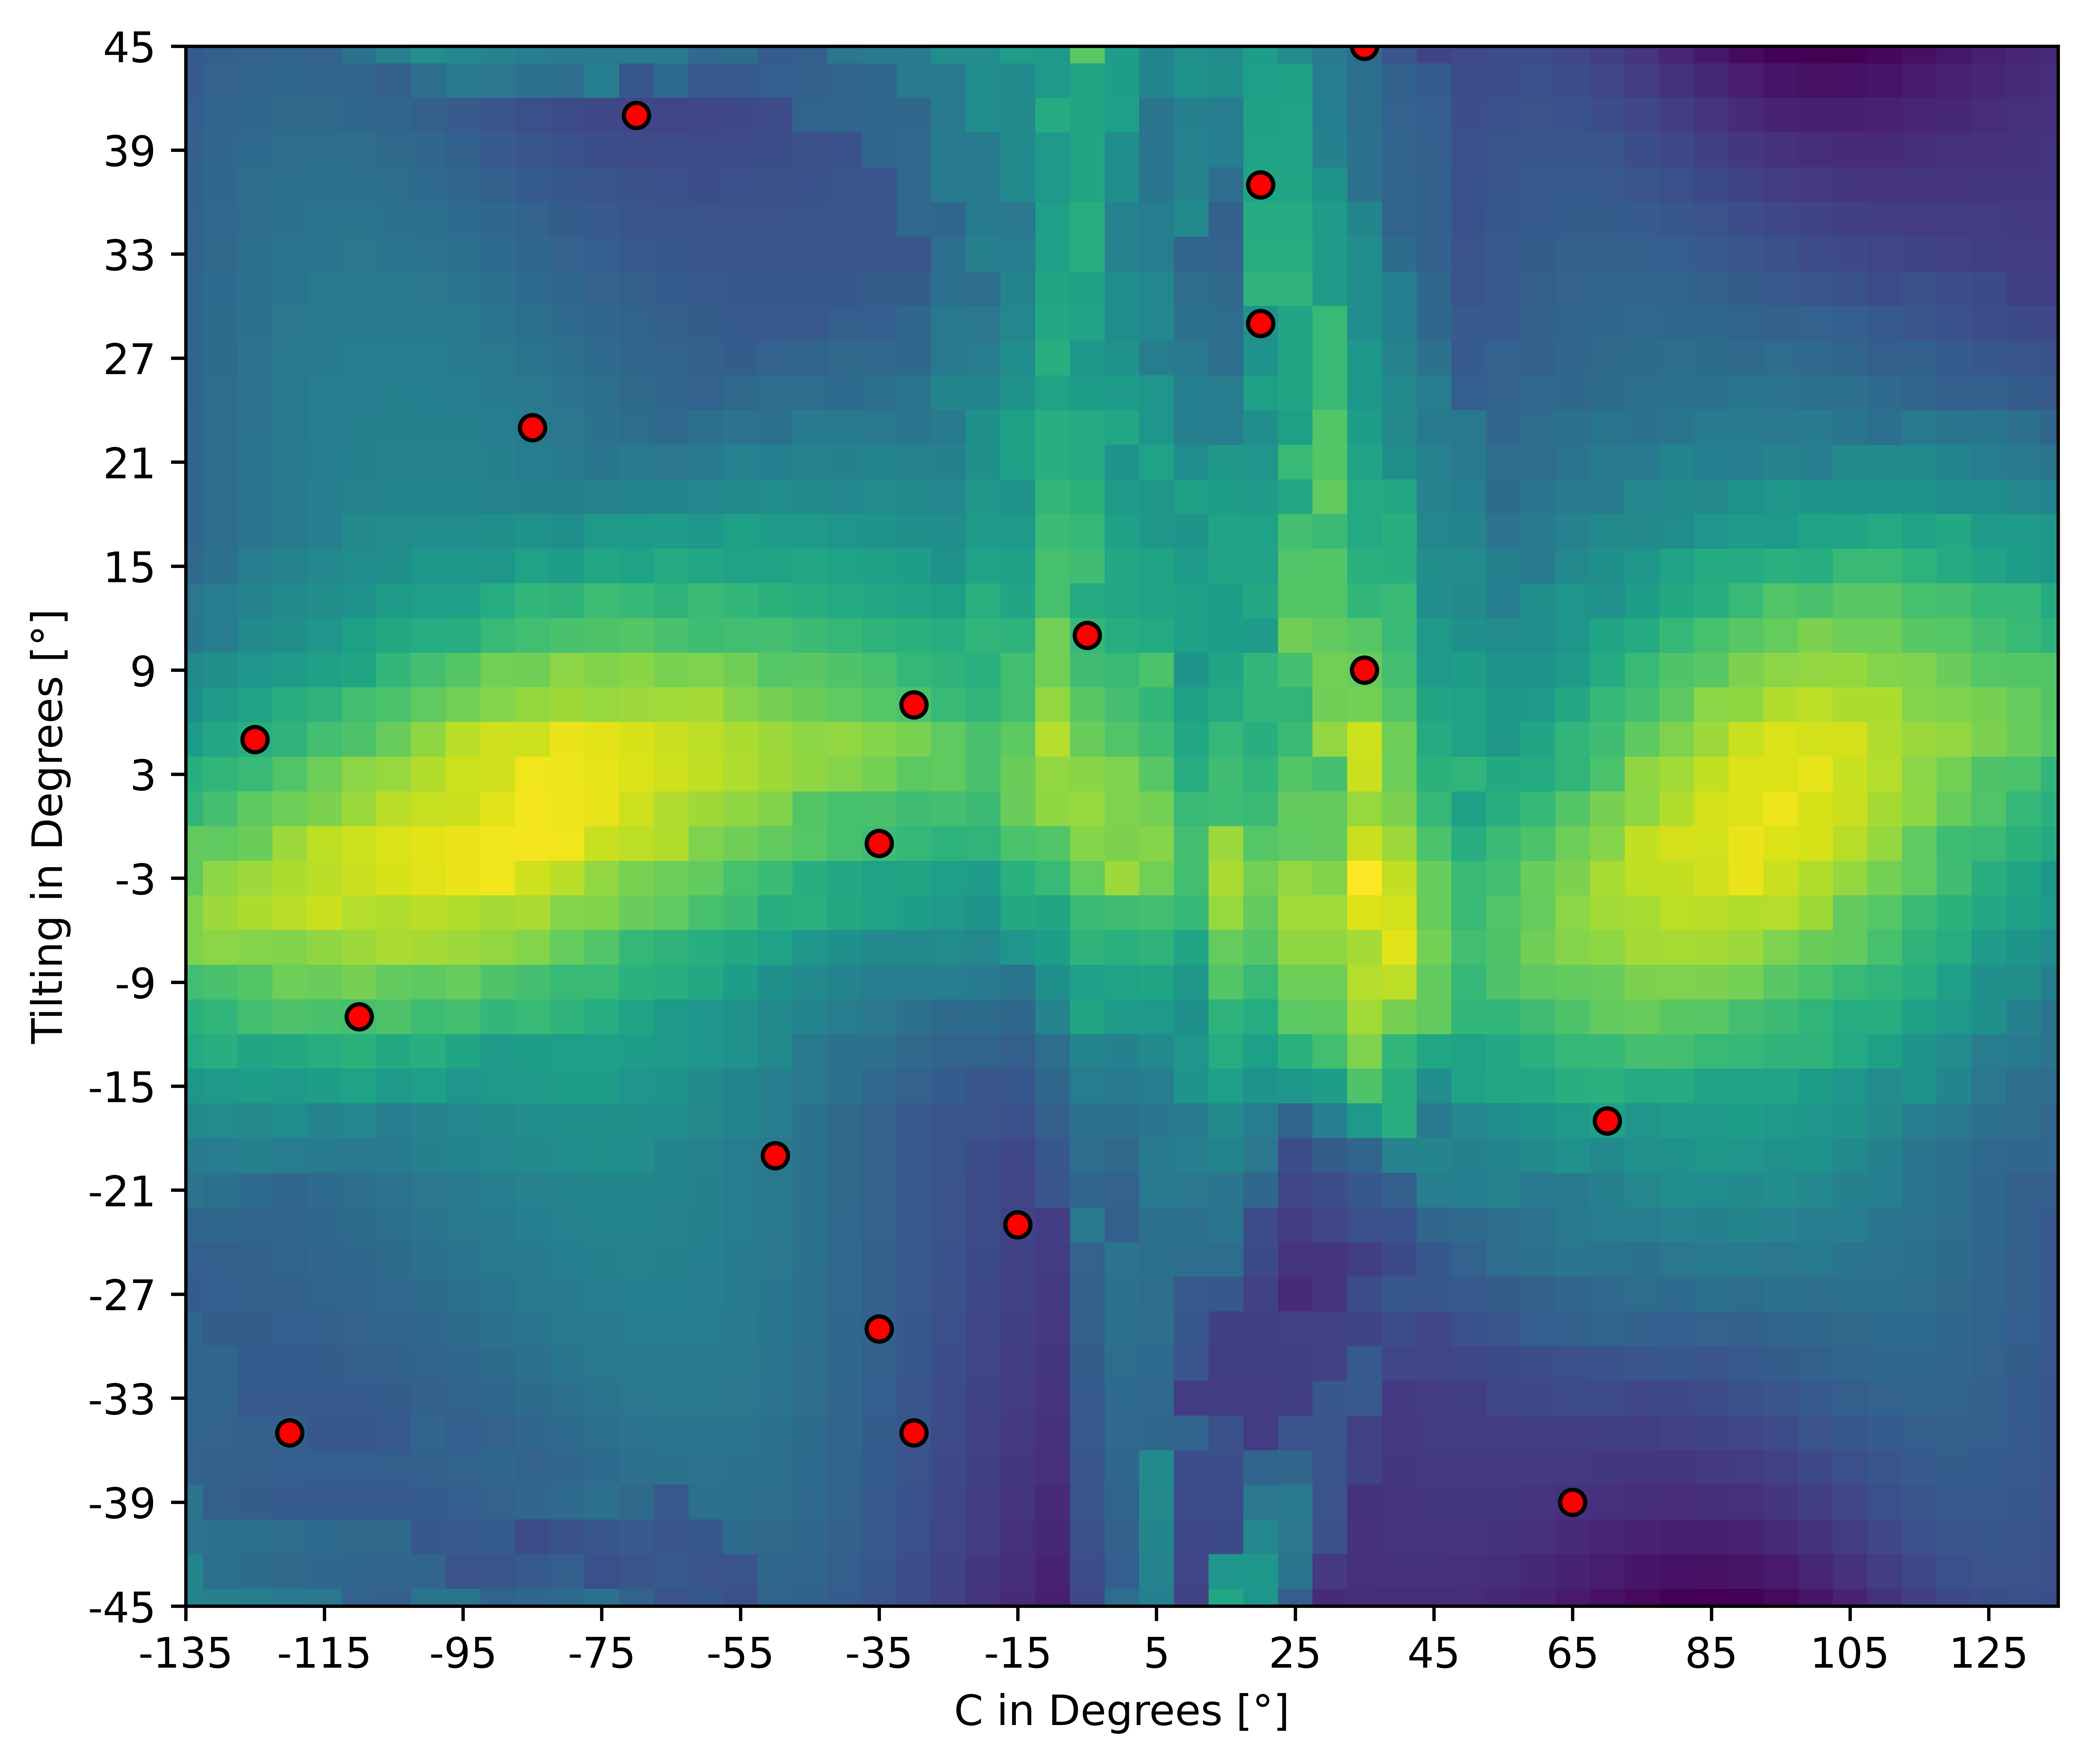
\includegraphics[width=0.7\textwidth]{figures/swarm/3_0.png}}
	\caption{Distributed of particles at their initial positions}
	\label{PSO_1}
\end{figure}



It is important to clarify that the individual particles in the \acrshort{PSO} algorithm do not have access to the entire global score matrix. The visualization of the global score matrix is only provided for the benefit of the human reader to aid in understanding. In reality, each particle only has knowledge of the global score at its own position. The particles update their positions iteratively by comparing their positions with each other. Each particle determines a new position based on the best score observed so far by all particles and the best score observed by itself. 

Figures \ref{2} to \ref{5} demonstrate the convergence of the particles towards the maximum global score. This convergence is achieved within 5 iterations. It is noteworthy that the best position of all 5 particles corresponds to the global maximum, as discussed in Chapter \ref{2RDOF}. This example highlights the ability to explore a high-dimensional space without the need to compute all possible combinations.


\begin{figure}[H]
	\centering
	\begin{minipage}{0.5\textwidth}
		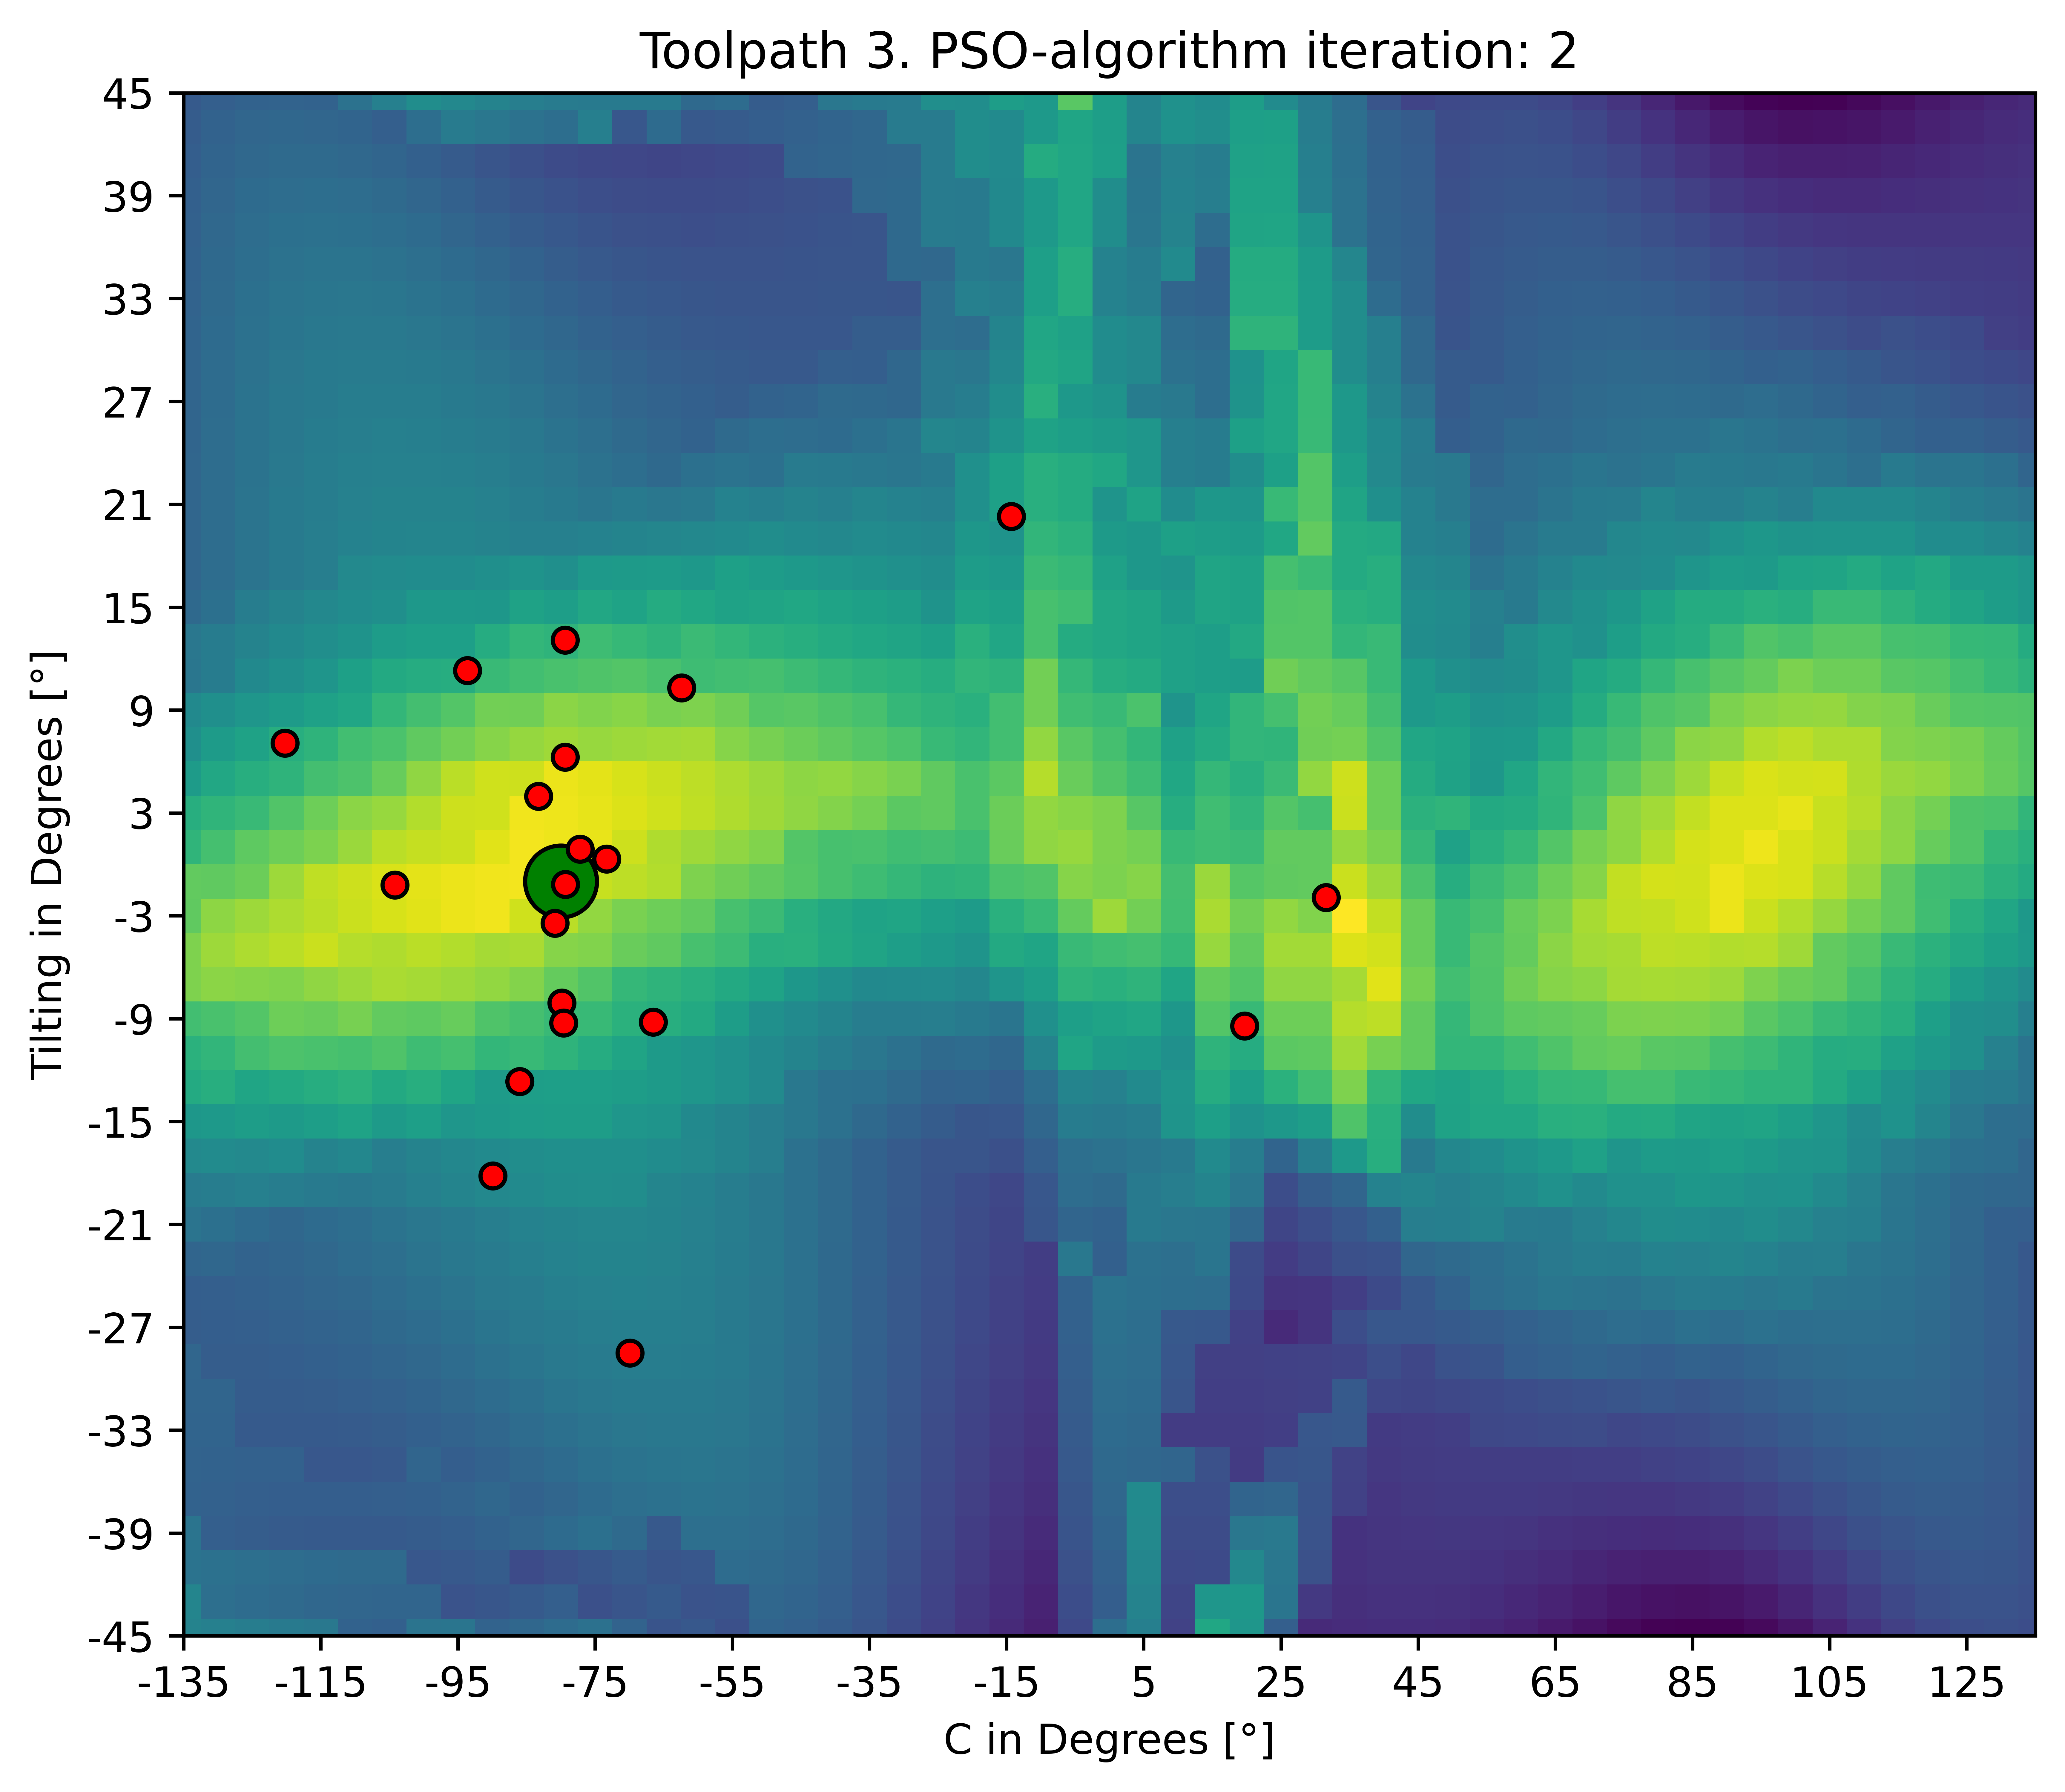
\includegraphics[width=\textwidth]{figures/swarm/3_2.png}
		\caption{PSO Iteration 2 on toolpath 3}
		\label{2}
	\end{minipage}\hfill
	\begin{minipage}{0.5\textwidth}
		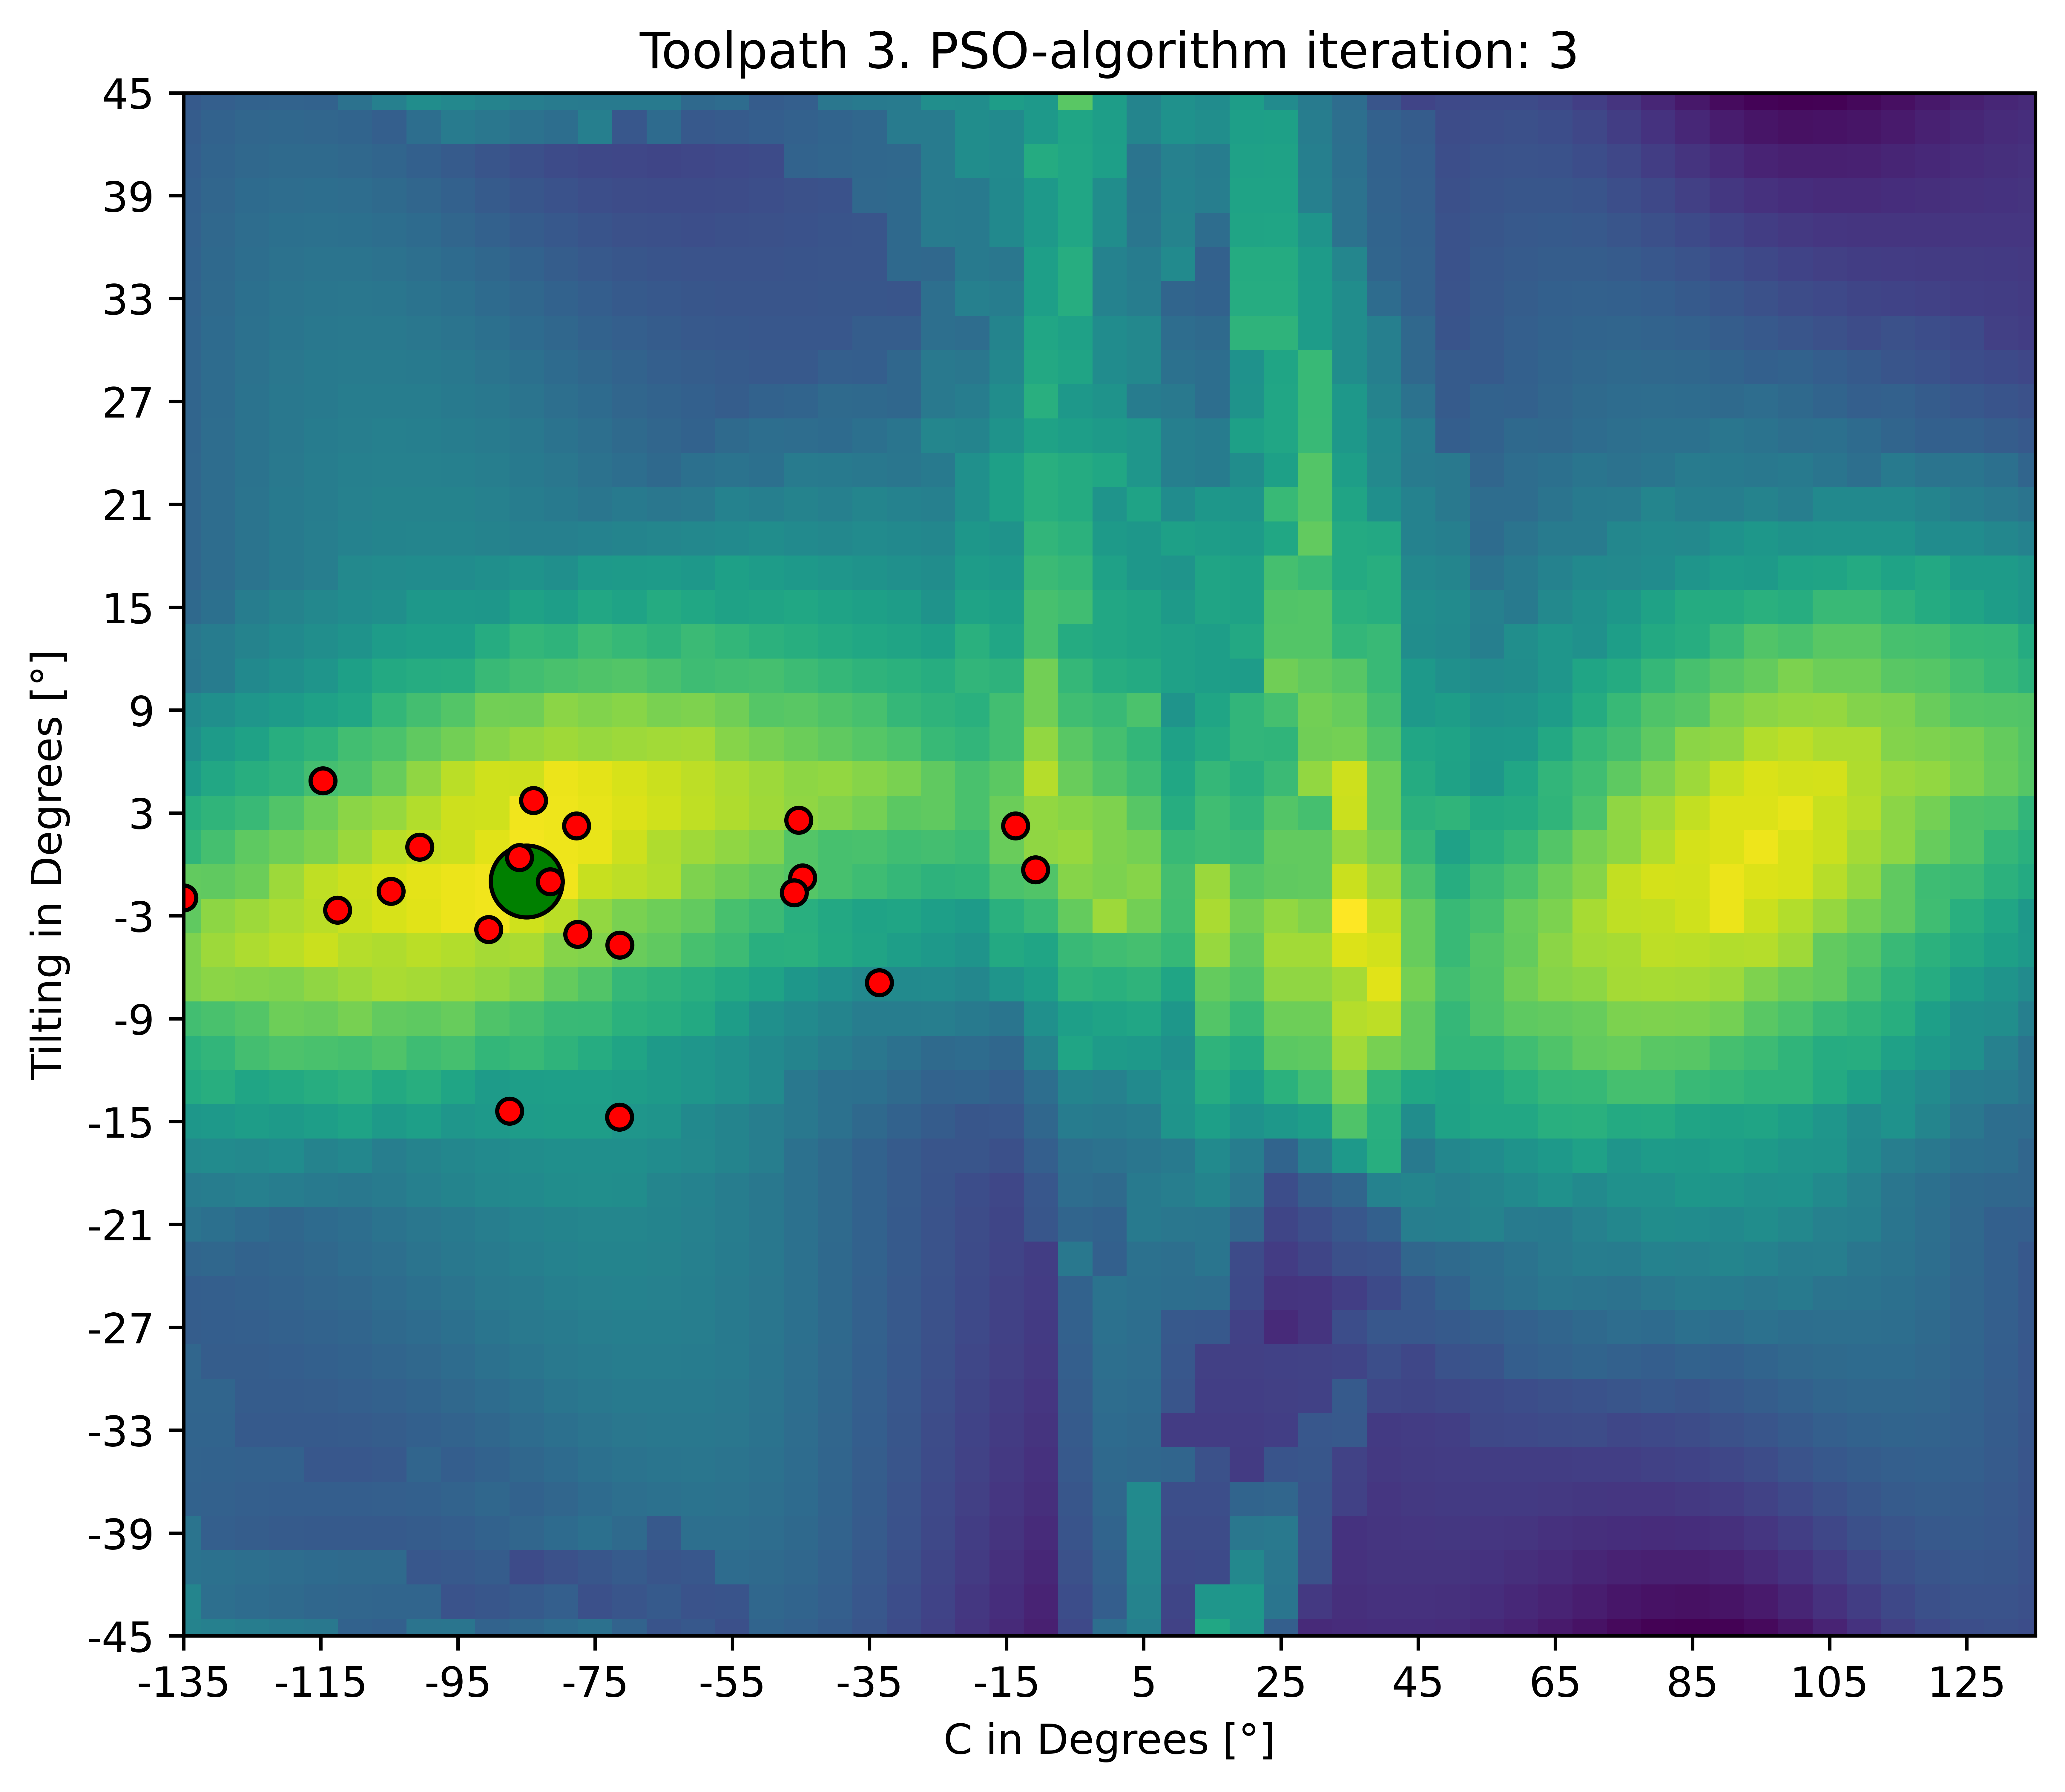
\includegraphics[width=\textwidth]{figures/swarm/3_3.png}
		\caption{PSO Iteration 3 on toolpath 3}
		\label{3}
	\end{minipage}\par
\end{figure}	


\begin{figure}[H]	
		\centering
	\begin{minipage}{0.5\textwidth}
		\includegraphics[width=\textwidth]{figures/swarm/3_4.png}
		\caption{PSO Iteration 4 on toolpath 3}
		\label{4}
	\end{minipage}\hfill
	\begin{minipage}{0.5\textwidth}
		\includegraphics[width=\textwidth]{figures/swarm/3_5.png}
		\caption{PSO Iteration 5 on toolpath 3}
		\label{5}
	\end{minipage}\par
\end{figure}
\newpage
One important consideration in this test is, that the scores have already been calculated. The global score matrix is determined by evaluating all possible combinations of different boundary conditions. However, in the intended scenario where this method is used to find the optimal boundary condition, such a pre-calculated matrix does not exist.

Therefore, in each iteration, the scores of the individual particle positions need to be compared relative to each other, taking into account the previous iterations. This process is illustrated in Figure \ref{swarmloop}. Initially, a predetermined number of particles is randomly placed on the plane, with the X and Y values representing the selected boundary conditions. For each selected boundary condition, the joint angles are calculated using the inverse kinematic approach. The analyzed process variables are then extracted and the joint angles are stored. The score for each current position is calculated relative to all stored toolpaths.

It is possible that in an early iteration, a particle had a position with a significantly higher score compared to the other available toolpaths. Therefore, after each iteration, it is necessary to update the score of the particle's most optimal position as more boundary conditions are analyzed. This is done to ensure that a score, which may have been mistakenly chosen as the best, does not influence the subsequent search directions.

\begin{figure}[H]
	\centerline{\includegraphics[width=1\textwidth]{figures/swarmloop.png}}
	\caption{PSO-Loop}
	\label{swarmloop}
\end{figure}

By utilizing this approach, the following results have been obtained. It is important to emphasize that the precalculated values of the global score matrix are not accessible to the \acrshort{PSO} algorithm. They are only used for evaluating the behavior of the particles and aiding in visualization. Figures \ref{1_true} to \ref{4_true} illustrate the evolution of the individual particles. The green circle represents the overall best position discovered by the particles up to that point
\newpage

\begin{figure}[H]
	\centering
	\begin{minipage}{0.5\textwidth}
		\includegraphics[width=\textwidth]{figures/swarm_true/3_1.png}
		\caption{PSO Iteration 1 on toolpath 3}
		\label{1_true}
	\end{minipage}\hfill
	\begin{minipage}{0.5\textwidth}
		\includegraphics[width=\textwidth]{figures/swarm_true/3_2.png}
		\caption{PSO Iteration 2 on toolpath 3}
		\label{2_true}
	\end{minipage}\par
\end{figure}	

\begin{figure}[H]	
	\centering
	\begin{minipage}{0.5\textwidth}
		\includegraphics[width=\textwidth]{figures/swarm_true/3_3.png}
		\caption{PSO Iteration 3 on toolpath 3}
		\label{3_true}
	\end{minipage}\hfill
	\begin{minipage}{0.5\textwidth}
		\includegraphics[width=\textwidth]{figures/swarm_true/3_4.png}
		\caption{PSO Iteration 4 on toolpath 3}
		\label{4_true}
	\end{minipage}\par
\end{figure}

The backtracking comparison of all previously visited positions by the particles is clearly evident in the movement of the green dot, which represents the best position found so far. As more points are visited by the particles, the calculation of the best boundary conditions improves. Even without the precalculated global score matrix, the particles are able to converge to the global optimum.
Figure \ref{5_true} illustrates the positions of the particles after the fifth and final iteration.
\newpage
\begin{figure}[H]
	\centerline{\includegraphics[width=0.8\textwidth]{figures/swarm_true/3_5.png}}
	\caption{PSO iteration 5 on toolpath 3}
	\label{5_true}
\end{figure}



The same optimization process can be applied to toolpath 1 and toolpath 2. The same process variables and weights are selected as for toolpath 3 (see Table \ref{PP_2}). Once again, 20 particles are analyzed over 5 iterations. Figures \ref{tp1_0} through \ref{tp1_5} depict the positions of the particles after the first and final iteration when analyzing the first toolpath, while Figures \ref{tp2_0} and \ref{tp2_5} showcase the initial and final positions of the particles when analyzing the second toolpath. In both cases, the PSO algorithm successfully converges very closely towards the optimal boundary condition.
\newpage
	
\begin{figure}[H]	
	\centering
	\begin{minipage}{0.5\textwidth}
		\includegraphics[width=\textwidth]{figures/swarm_true/1_1.png}
		\caption{PSO Iteration 1 on toolpath 1}
		\label{tp1_0}
	\end{minipage}\hfill
	\begin{minipage}{0.5\textwidth}
		\includegraphics[width=\textwidth]{figures/swarm_true/1_5.png}
		\caption{PSO Iteration 5 on toolpath 1}
		\label{tp1_5}
	\end{minipage}\par
\end{figure}


\begin{figure}[H]	
	\centering
	\begin{minipage}{0.5\textwidth}
		\includegraphics[width=\textwidth]{figures/swarm_true/2_1.png}
		\caption{PSO Iteration 1 on toolpath 2}
		\label{tp2_0}
	\end{minipage}\hfill
	\begin{minipage}{0.5\textwidth}
		\includegraphics[width=\textwidth]{figures/swarm_true/2_5.png}
		\caption{PSO Iteration 5 on toolpath 2}
		\label{tp2_5}
	\end{minipage}\par
\end{figure}



\newpage
\section{Analysis and Discussion of the Results}%
In the following, the results are analyzed in detail and critically discussed.

\subsection{Summary and Analysis of the Results}
When analyzing only one redundant \acrshort{DoF}, specifically the rotation around the Z-axis (see Figure \ref{GS1}, Figure \ref{TP2_combi}, and Figure \ref{TP3_combi}), it becomes evident that there is significant potential for improvement. In this initial test, the process variables "direction changes in all joints," "total travel in all joints," and "acceleration in joint 1" are analyzed. The local score for "total travel in all joints" and "acceleration in joint 1" both exhibit a very continuous change over the entire range of the analyzed rotation. This characteristic is a clear indication that optimization algorithms are a reasonable choice for finding the optimal boundary condition.

To further validate the proposed method for analyzing process variables, a production-grade G-Code is examined (see Figure \ref{LS4}). This G-Code consists of 28,000 coordinates and takes significantly longer to analyze. The resulting comparison of all possible values for the redundant \acrshort{DoF} shows a fairly smooth curve of the global score. It is important to note that the local score for the direction changes in all analyzed toolpaths is not as smooth as the other analyzed variables.


When considering the scenario where two \acrshort{DoF} can be set, it is observed that toolpath 1 and toolpath 2 have very similar boundary conditions for the global optimum (see Figure \ref{best_2D_1} and Figure \ref{best_2D_2}). This suggests that these two toolpaths do not differ significantly from each other when considering the process variables alone. 

Analyzing the hyperplane of toolpath 1 (Figure \ref{best_2D_1}), it is clearly visible that most of the possible combinations result in a very high global score. The combinations that lead to a low local score form a ravine that is clearly visible on the right-hand side. In the case of toolpath~2 (Figure \ref{best_2D_2}), distinct streaks can be observed. The middle of the matrix represents a continuous region, while multiple discontinuities occur on the sides. Toolpath 3 (Figure \ref{best_2D}) exhibits an almost symmetrical hyperplane. Two local optima are visible on the left and right sides, while the middle part consists of a jagged area with many non-smooth jumps. It is worth noting that the calculation of each individual global score matrix takes approximately 1 hour.


Based on the results obtained from the \acrshort{PSO} algorithm (see Figure \ref{5_true}), it can be concluded that achieving a close-to-optimal result is feasible when the global score matrix yields smooth surfaces. By implementing this approach, a significant reduction in computation time is possible. Instead of calculating the entire matrix, only 100 toolpaths need to be computed using the inverse kinematics algorithm, resulting in a computation time of just 15 minutes.

The number of particles is selected to be as high as possible while also considering the computational costs. Rather than increasing the number of particles, the number of iterations is set to 5 in order to facilitate convergence towards the global optima. The results clearly show that such a convergence is possible.


%NO \acrshort{CAM} EXPLAIN








\subsection{Discussion of the Results}%


Even though the results show a very promising outcome, it is necessary to consider some additional factors. One of the most obvious elements is that only three artificial and one production-grate toolpaths are analyzed. To validate this method in detail, it is necessary to use more real-life production G-code with correctly modeled robotic systems and analyze whether it can be optimized. It should be noted that this work only provides a limited excerpt and does not analyze complex multi-axis operations, which are a significant advantage and building block of the \acrshort{WAAM} process.

The selected inverse kinematics algorithm is not designed for optimal high-performance calculations, making it infeasible to use when dealing with toolpaths that have millions of coordinates. Additionally, the algorithm calculates the joint position numerically rather than analytically, which can result in unexpected robot poses. \acrshort{CAM} software such as \textit{Siemens NX} or \textit{Master CAM} offer additional options for inverse kinematics that can be used to fine-tune the behavior of the robot.

When analyzing multiple process variables, it is not guaranteed that the resulting surface will be smooth and optimal for the selected optimization algorithm. Additionally, when working with a \acrshort{PSO} algorithm, the final result strongly depends on the initial distribution of the particles. If the optimum is a very tight and sharp spike, the probability of finding the optimal boundary condition is significantly lower. This is particularly true in systems with 3 or more redundant \acrshort{DoF}, where simple optimization algorithms can lead to suboptimal results or require unfeasibly long computation times. When implementing the \acrshort{PSO} algorithm, 20 particles over 5 iterations are analyzed. In future work, it is necessary to analyze how a increase in population size will improve the convergence rate. 

When analyzing Figure \ref{GS1}, Figure \ref{TP2_combi}, and Figure \ref{TP3_combi}, it becomes evident that the best boundary conditions for the highest global score are very similar. Both toolpath 1 and 2 have an optimum of -120°, while toolpath 3 has an optimum at -90°. This suggests that there could be an optimal robot configuration that is applicable to any toolpath.

In general, the presented methodology does provide a solid basis as a proof of concept for the proposed method. However, additional implementations and test are necessary for it to be feasible in an industrial environment.
%% ADD ME !!!!!!!!!!!!!!!!!!!!
%% !TeX spellcheck = en_US
\chapter{Conclusion}%

\section{Summary}%

\section{Outlook}%
		Cycle time 
		%Another important parameter is the cycle time, which represents the time required to execute the G-code. Various factors can influence the cycle time, such as feed rates, engagement depth of a cutting tool, or wire feed rates in the case of additive manufacturing processes. By adjusting these parameters, manufacturers can significantly reduce or increase the cycle time, optimizing the efficiency and productivity of the manufacturing process.
		
		%Analyzing and optimizing the cycle time helps to streamline operations, reduce production time, and enhance overall productivity. It allows manufacturers to identify opportunities for improvement and make informed decisions regarding process parameters, leading to increased throughput and cost savings.
		
				Stiffness value
				
				%Another crucial factor in industrial robot tool path execution is the stiffness value. This value specifically refers to the stiffness in the direction of the highest contact forces, or the most critical direction. In certain machining scenarios, such as when cutting a slot with full engagement, the stiffness in the cutting direction may be of lesser importance compared to the stiffness in the perpendicular direction of the cut.
				
				%Maintaining high stiffness in the orthogonal cutting direction is vital, as it helps minimize deviations from the desired mid-axis of the slot. Conversely, when high contact forces are combined with low stiffness, it can result in significant deviations in the final dimensions of the machined part.
				%To determine the stiffness value, a finite-element analysis, multi-body simulation or CAM simulation can be employed. These simulations provide the necessary data, which is also stored in the form of an array, to extract the stiffness values for analysis and optimization purposes.
				
				
						Collision index

%The collision index is used to determine if any potential collisions could occur between any part of the robot or the end-effector and the workpieces or other objects in the environment. This parameter is particularly important in scenarios involving WAAM systems, where loose wires can change their position depending on the robot's pose. It helps to prevent potential collisions that could lead to damage to the workpiece, the robot, or other equipment.

Man kann im Ausblick zeigen, dass ein Bauteil-Verschieben auch eine Verbesserung bringen kann, aber das ist erstmal nicht der Fokus

ML for best case calculations – Oultook?)%% ADD ME !!!!!!!!!!!!!!!!!!!!
%
% Appendix
% --------
%\appendix%
%\chapter{Appendix}%

%
%

%\listoffigures % ADD ME !!!!!!!!!!!!!!!!!!!!
%\listoftables
% Glossary
% ---------------------
%\printnoidxglossary[sort=standard,title={\IWBlangGlossary}]
%
% References
% ----------
!\printbibliography[heading=bibintoc, title={\IWBlangBibliography}]%

%
%
\end{document}%
%
%
